% Options for packages loaded elsewhere
\PassOptionsToPackage{unicode}{hyperref}
\PassOptionsToPackage{hyphens}{url}
%
\documentclass[
]{article}
\usepackage{lmodern}
\usepackage{amssymb,amsmath}
\usepackage{ifxetex,ifluatex}
\ifnum 0\ifxetex 1\fi\ifluatex 1\fi=0 % if pdftex
  \usepackage[T1]{fontenc}
  \usepackage[utf8]{inputenc}
  \usepackage{textcomp} % provide euro and other symbols
\else % if luatex or xetex
  \usepackage{unicode-math}
  \defaultfontfeatures{Scale=MatchLowercase}
  \defaultfontfeatures[\rmfamily]{Ligatures=TeX,Scale=1}
\fi
% Use upquote if available, for straight quotes in verbatim environments
\IfFileExists{upquote.sty}{\usepackage{upquote}}{}
\IfFileExists{microtype.sty}{% use microtype if available
  \usepackage[]{microtype}
  \UseMicrotypeSet[protrusion]{basicmath} % disable protrusion for tt fonts
}{}
\usepackage{xcolor}
\IfFileExists{xurl.sty}{\usepackage{xurl}}{} % add URL line breaks if available
\IfFileExists{bookmark.sty}{\usepackage{bookmark}}{\usepackage{hyperref}}
\hypersetup{
  pdftitle={Estimating the reliability of components in a series systems from masked failure data},
  pdfauthor={Alex Towell},
  hidelinks,
  pdfcreator={LaTeX via pandoc}}
\urlstyle{same} % disable monospaced font for URLs
\usepackage[margin=1in]{geometry}
\usepackage{color}
\usepackage{fancyvrb}
\newcommand{\VerbBar}{|}
\newcommand{\VERB}{\Verb[commandchars=\\\{\}]}
\DefineVerbatimEnvironment{Highlighting}{Verbatim}{commandchars=\\\{\}}
% Add ',fontsize=\small' for more characters per line
\usepackage{framed}
\definecolor{shadecolor}{RGB}{248,248,248}
\newenvironment{Shaded}{\begin{snugshade}}{\end{snugshade}}
\newcommand{\AlertTok}[1]{\textcolor[rgb]{0.94,0.16,0.16}{#1}}
\newcommand{\AnnotationTok}[1]{\textcolor[rgb]{0.56,0.35,0.01}{\textbf{\textit{#1}}}}
\newcommand{\AttributeTok}[1]{\textcolor[rgb]{0.77,0.63,0.00}{#1}}
\newcommand{\BaseNTok}[1]{\textcolor[rgb]{0.00,0.00,0.81}{#1}}
\newcommand{\BuiltInTok}[1]{#1}
\newcommand{\CharTok}[1]{\textcolor[rgb]{0.31,0.60,0.02}{#1}}
\newcommand{\CommentTok}[1]{\textcolor[rgb]{0.56,0.35,0.01}{\textit{#1}}}
\newcommand{\CommentVarTok}[1]{\textcolor[rgb]{0.56,0.35,0.01}{\textbf{\textit{#1}}}}
\newcommand{\ConstantTok}[1]{\textcolor[rgb]{0.00,0.00,0.00}{#1}}
\newcommand{\ControlFlowTok}[1]{\textcolor[rgb]{0.13,0.29,0.53}{\textbf{#1}}}
\newcommand{\DataTypeTok}[1]{\textcolor[rgb]{0.13,0.29,0.53}{#1}}
\newcommand{\DecValTok}[1]{\textcolor[rgb]{0.00,0.00,0.81}{#1}}
\newcommand{\DocumentationTok}[1]{\textcolor[rgb]{0.56,0.35,0.01}{\textbf{\textit{#1}}}}
\newcommand{\ErrorTok}[1]{\textcolor[rgb]{0.64,0.00,0.00}{\textbf{#1}}}
\newcommand{\ExtensionTok}[1]{#1}
\newcommand{\FloatTok}[1]{\textcolor[rgb]{0.00,0.00,0.81}{#1}}
\newcommand{\FunctionTok}[1]{\textcolor[rgb]{0.00,0.00,0.00}{#1}}
\newcommand{\ImportTok}[1]{#1}
\newcommand{\InformationTok}[1]{\textcolor[rgb]{0.56,0.35,0.01}{\textbf{\textit{#1}}}}
\newcommand{\KeywordTok}[1]{\textcolor[rgb]{0.13,0.29,0.53}{\textbf{#1}}}
\newcommand{\NormalTok}[1]{#1}
\newcommand{\OperatorTok}[1]{\textcolor[rgb]{0.81,0.36,0.00}{\textbf{#1}}}
\newcommand{\OtherTok}[1]{\textcolor[rgb]{0.56,0.35,0.01}{#1}}
\newcommand{\PreprocessorTok}[1]{\textcolor[rgb]{0.56,0.35,0.01}{\textit{#1}}}
\newcommand{\RegionMarkerTok}[1]{#1}
\newcommand{\SpecialCharTok}[1]{\textcolor[rgb]{0.00,0.00,0.00}{#1}}
\newcommand{\SpecialStringTok}[1]{\textcolor[rgb]{0.31,0.60,0.02}{#1}}
\newcommand{\StringTok}[1]{\textcolor[rgb]{0.31,0.60,0.02}{#1}}
\newcommand{\VariableTok}[1]{\textcolor[rgb]{0.00,0.00,0.00}{#1}}
\newcommand{\VerbatimStringTok}[1]{\textcolor[rgb]{0.31,0.60,0.02}{#1}}
\newcommand{\WarningTok}[1]{\textcolor[rgb]{0.56,0.35,0.01}{\textbf{\textit{#1}}}}
\usepackage{longtable,booktabs}
% Correct order of tables after \paragraph or \subparagraph
\usepackage{etoolbox}
\makeatletter
\patchcmd\longtable{\par}{\if@noskipsec\mbox{}\fi\par}{}{}
\makeatother
% Allow footnotes in longtable head/foot
\IfFileExists{footnotehyper.sty}{\usepackage{footnotehyper}}{\usepackage{footnote}}
\makesavenoteenv{longtable}
\usepackage{graphicx}
\makeatletter
\def\maxwidth{\ifdim\Gin@nat@width>\linewidth\linewidth\else\Gin@nat@width\fi}
\def\maxheight{\ifdim\Gin@nat@height>\textheight\textheight\else\Gin@nat@height\fi}
\makeatother
% Scale images if necessary, so that they will not overflow the page
% margins by default, and it is still possible to overwrite the defaults
% using explicit options in \includegraphics[width, height, ...]{}
\setkeys{Gin}{width=\maxwidth,height=\maxheight,keepaspectratio}
% Set default figure placement to htbp
\makeatletter
\def\fps@figure{htbp}
\makeatother
\setlength{\emergencystretch}{3em} % prevent overfull lines
\providecommand{\tightlist}{%
  \setlength{\itemsep}{0pt}\setlength{\parskip}{0pt}}
\setcounter{secnumdepth}{5}
\usepackage{graphicx}
\usepackage{amsthm}
\usepackage{amsmath}
\usepackage{natbib}
\usepackage{tikz}
\newlength{\cslhangindent}
\setlength{\cslhangindent}{1.5em}
\newenvironment{cslreferences}%
  {}%
  {\par}

\title{Estimating the reliability of components in a series systems from
masked failure data}
\author{Alex Towell}
\date{}

\begin{document}
\maketitle
\begin{abstract}
We estimate the reliability of series systems from masked failure data
consisting of right-censored system lifetimes and masked component cause
of failures. Under a minimal set of conditions that permit us to ignore
how the component cause of failures are masked, we estimate the sampling
distribution of the MLE in a variety of situations. We find that as long
as the masking does not always include a particular component as a
potential cause of failure whenever another component is also a
potential cause, the MLE is unique and consistent. However, this is
often not a realistic situation in industrial settings. For example, a
system may be repaired by replacing an entire circuit board consisting
of multiple components, in which case whenever one of the components on
that circuit board fails, all of the components on the circuit board are
potential component causes of failure. In this case, we have a
non-unique MLE, which provides less information about the reliability of
the series system and its components.
\end{abstract}

{
\setcounter{tocdepth}{2}
\tableofcontents
}
\newcommand{\T}{T}
\newtheorem{definition}{Definition}
\newtheorem{theorem}{Theorem}
\newtheorem{corollary}{Corollary}
\newtheorem{condition}{Condition}
\renewcommand{\v}[1]{\boldsymbol{#1}}
\numberwithin{equation}{section}

\hypertarget{introduction}{%
\section{Introduction}\label{introduction}}

Accurate reliability specifications of components of a multi-component
system, such as mean time to failure (MTTF), can be quite valuable. For
instance, such information may be used to help identify the component
cause of system failure. However, this information is often not
available, or if it is available, it may not be very accurate. In this
case, we may try to estimate the reliability of each component from
system failure data.

We are interested in estimating the reliability of \emph{series
systems}. In a series system, the system fails whenever any of its
components fail. The famous statistician George Box once opined that all
models are wrong, but some are useful, meaning that a theoretical model
of real phenomenon is incapable of representing its exact behaviour, but
it may still be useful. Indeed, sometimes it is even more useful, since
a simplified model is more understandable and only includes the most
salient features.

Since many real-world systems are greatly impaired whenever a set of its
\emph{critical} components fail, the series system model is often a very
\emph{useful} approximation of its internal structure. For example,
people in a particular experiment may be regarded as series systems
where the components are some relevant set of vital organs. This model
is often a very useful abstraction that averages over many complicated,
unobserved details that may only have a small effect on an average
person's lifespan.

In this paper, the experimental unit is a particular type of series
system that consists of \(m\) components and we seek to estimate the
reliability of the components from \emph{masked data} where we observe
only partial information about the system, e.g., the component lifetimes
are masked (not observed in the sample).

We imagine that we conduct an experiment where we obtain the lifetimes
of the \(m\) components, which has a sample space \((0,\infty)^m\). An
observed result is called an \emph{outcome} of the experiment, e.g.,
\((1.2,0.5,1.1)\). However, we assume that this data is masked in the
following ways:

\begin{enumerate}
\def\labelenumi{\arabic{enumi}.}
\item
  The experiments may be right-censored, which means that the experiment
  or observation may be suspended before the system fails.
\item
  We can only observe the lifetime of the component with the minimum
  lifetime. This constraint is imposed by the fact that the system is
  arranged in series and thus stops working whenever one of the
  components fails.
\item
  It may not be easy or possible to identify the failed component. We
  consider the case where we can only observe a set of components that
  includes the failed component. We refer to this set of components as
  the candidate set.\footnote{
  If the candidate set has only a single component, then we know the exact
  component cause of failure.}

  This constraint may be due to a variety of reasons. A canonical
  example is given by supposing that when the series system fails, it is
  repaired by simultaneously replacing some subset of the components,
  thus preventing isolating the specific failed component.
\end{enumerate}

We take a random sample of \(n\) such experiments, where the
right-censored system lifetimes are i.i.d. when conditioned on the
right-censoring time, but the candidate sets are assumed to be
independent but not necessarily identically distributed. In later
sections, we consider a set of realistic conditions that allow us to
ignore the distribution of candidate sets, which allows us to construct
a reduced likelihood function for the masked failure data. Finally, we
find the MLE \(\hat{\boldsymbol{\theta}}\) that maximizes the reduced
likelihood function, which is the same MLE for ``full'' likelihood
function where we know the distribution of candidate sets.

\hypertarget{sec:statmod}{%
\section{Statistical model}\label{sec:statmod}}

Consider a system with \(m\) components, indexed by \(1,2,\ldots,m\).
Each component only has two possible states, \emph{failed} and
\emph{functioning}. The state of the system also only has two possible
states, \emph{failed} and \emph{functioning}. The lifetime of a system
is the elapsed time from when the new, functioning system is put into
operation until it fails for the \emph{first time}. We are not
interested in what happens to a system after it fails, e.g., we do not
consider repairing systems and putting them back into operation under
further observation.

A system that is in a functioning state if and only if at least \(k\) of
the \(m\) components are in a functioning state is denoted a
\(k\)-out-of-\(m\) system. We narrow our scope to \(m\)-out-of-\(m\)
systems, also known as \emph{series systems} (with \(m\) components). A
series system is functioning if and only if every component is
functioning. Consequently, in a series system, precisely one component
is the cause of failure.

Our sample consists of lifetime data for i.i.d. series systems. Since
the component lifetimes are subject to chance variations, we denote the
lifetime of the \(j\)\textsuperscript{th} component of the
\(i\)\textsuperscript{th} system by the random variable \(T_{i j}\). We
assume that the \(m\) component lifetimes, \(T_{i 1},\ldots,T_{i m}\),
are statistically independent and non-identical. In a series system,
whenever any component fails, the system fails. Thus, the lifetime of
the \(i\)\textsuperscript{th} system, \(T_i\), is given by the component
with the smallest lifetime, \[
    T_i = \min\bigr\{T_{i 1},T_{i 2}, \ldots, T_{i m} \bigr\}.
\]

We assume that the component lifetimes may be adequately modeled by some
parametric probability distribution. In what follows, matrices and
vectors are denoted in boldface, e.g., \(\boldsymbol{x}\) is a vector.
The \(i\)\textsuperscript{th} column and \((i,j)\)-th element of a
matrix \(\boldsymbol{A}\) is denoted respectively by
\(\boldsymbol{A_j}\) and \(\boldsymbol{A}_{i j}\). We let
\(\boldsymbol{\theta_j}\) denote the parameter vector of the
\(j\textsuperscript{th}\) component, and each \(\boldsymbol{\theta_j}\)
for \(j=1,\ldots,m\) may be different sizes. We define the parameter
vector of the entire series system by \[
    \boldsymbol{\theta }= (\boldsymbol{\theta_1},\ldots,\boldsymbol{\theta_m}).
\]

The cumulative distribution function (cdf) for a random varible \(T\) is
given by \begin{equation}
 F_T(t) = \Pr\{T \leq t\},
\end{equation} where \(\Pr\{T \in E\}\) denotes the probability that a
random variable \(T\) realizes a value in \(E\). If a random variable
\(X\) is discrete, then its probability mass function (pmf) \(f_X\) is
given by\(f_X(x) = \Pr\{X = x\}\). The probability density function
(pdf) for a continuous random varible \(T\) is given by \begin{equation}
f_T(t) = \frac{d}{dt} F_T(t).
\end{equation}

If a random variable \(T\) has a parametric distribution indexed by a
parameter vector \(\boldsymbol{\beta}\), we denote its pdf by
\(f_T(t;\boldsymbol{\beta})\) and likewise for other distribution
functions, e.g., the \(i\)\textsuperscript{th} series system has a cdf
denoted by \(F_{T_i}(t;\boldsymbol{\theta})\). In the case of the
lifetime distribution functions of components, we subscript the
distribution functions by component index instead of the symbol for the
random variable, e.g., the cdf of the \(j\)\textsuperscript{th}
component for the \(i\)-th system is denoted by
\(F_j(t;\boldsymbol{\theta_j})\) instead of
\(F_{T_{i j}}(t;\boldsymbol{\theta_j})\). If it is clear from the
context which random variable a distribution function is for, we may
drop the subscripts, e.g., \(F(t)\) instead of \(F_T(t)\). Finally, as
an abuse of notation, we often write a function as \(f(t)\) when we
really mean that \(f\) is a function of variable \(t\).

There are two particularly important functions in survival analysis, the
survival function and the hazard function.

\begin{definition}
The survival function, $R_T(t)$, of a random lifetime $T$ is the
probability that it realizes a value larger than some specified duration of time $t$,
\begin{equation}
\begin{split}
R_T(t) &= \Pr\{T > t\}\\
     &= 1 - F_T(t).
\end{split}
\end{equation}
In other words, $R_T(t)$ denotes the probability that $T$ survives longer than
$t$.
\end{definition}

The hazard function is a bit more subtle. For a random lifetime \(T\),
the probability that a failure occurs between \(t\) and \(\Delta t\)
given that no failure occurs before time \(t\) is given by \[
\Pr\{T \leq t+\Delta t|T > t\} = \frac{\Pr\{t < T < t+\Delta t\}}{\Pr\{T > t\}}.
\] The \emph{failure rate} is given by the above divided by the length
of the time interval, \(\Delta t\): \[
\frac{\Pr\{t < T < t+\Delta t\}}{\Delta t} \frac{1}{\Pr\{T > t\}} =
    \frac{R_T(t) - R(t+\Delta t)}{R_T(t)}.
\]

\begin{definition}
\label{def:failure_rate}
The hazard function $h_T(t)$ for a continuous random variable $T$ is the
instantaneous failure rate at time $t$, which is given by
\begin{equation}
\label{eq:failure_rate}
\begin{split}
h_T(t) &= \lim_{\Delta t \to 0} \frac{\Pr\{t < T < t+\Delta t\}}{\Delta t} \frac{1}{\Pr\{T > t\}}\\
       &= \frac{f_T(t)}{R_T(t)}.
\end{split}
\end{equation}
\end{definition}

Two random variables \(X\) and \(Y\) have a joint pdf \(f_{X,Y}(x,y)\).
Given the joint pdf \(f(x,y)\), the marginal pdf of \(X\) is given by \[
f_X(x) = \int_{\mathcal{Y}} f_{X,Y}(x,y) dy,
\] where \(\mathcal{Y}\) is the support of \(Y\). (If \(Y\) is discrete,
replace the integration with a summation over \(\mathcal{Y}\).)

The conditional pdf of \(Y\) given \(X=x\), \(f_{Y|X}(y|x)\), is defined
as \[
f_{X|Y}(y|x) = \frac{f_{X,Y}(x,y)}{f_X(x)}.
\] We may generalize all of the above to more than two random variables,
e.g., the joint pdf of \(X_1,\ldots,X_m\) is denoted by
\(f(x_1,\ldots,x_m)\).

\hypertarget{sec:data}{%
\subsection{Masked data}\label{sec:data}}

The object of interest is the (unknown) parameter value
\(\boldsymbol{\theta}\). To estimate this \(\boldsymbol{\theta}\), we
need \emph{data}. Generally, we encounter three types of life data in
this context: exact lifetimes, interval lifetimes (in which a lifetime
is known to have occurred between two points in time), and right
censored lifetimes (in which we only know that a lifetime is greater
than some point in time, e.g., the experiment was terminated or
suspended before the system failed).

In this paper, we limit our focus to right censored lifetimes. We
consider a sample of \(n\) i.i.d. series systems, each of which is put
into operation at some time and and observed until either it fails or is
right-censored.

We denote the right-censoring time of the \(i\)\textsuperscript{th}
system by \(\tau_i\). Whether it is right-censored is a random variable
defined as \begin{equation}
    \delta_i = 1_{T_i < \tau_i}
\end{equation} where \(1_{\text{condition}}\) is an indicator function
that outputs \(1\) if \emph{condition} is true and \(0\) otherwise.
Here, \(\delta_i = 1\) indicates the event of interest, a system
failure, was observed. The right-censored time of the
\(i\)\textsuperscript{th} system, \(S_i\), is given by \begin{equation}
    S_i = \min\{\tau_i, T_i\}.
\end{equation}

In addition to the above, we also have masked data about the component
cause of failure in the form of candidate sets. A candidate set consists
of some subset of component indices that plausibly contain the index of
the failed component. The sample space of candidate sets are all subsets
of \(\{1,\ldots,m\}\), thus there are \(2^m\) possible outcomes in the
sample space.

Let's define the candidate set corresponding to the
\(i\)\textsuperscript{th} system as \(c_i\). Since the data generating
process for candidate sets may be subject to chance variations, we model
it as a random set \(\mathcal{C}_i\). We may also represent the
candidate set \(\mathcal{C}_i\) as a random Boolean vector
\(X_{i 1},\ldots,X_{i m}\) where \(X_{i j}=1\) denotes that the
\(j\)\textsuperscript{th} component index is in the candidate set for
the \(i\)\textsuperscript{th} system.

When we refer to the sequence \(a_1,\ldots,a_k\), we use the notation
\(\{a_i\}_{i \leq k}\). If it is clear from the context, we may also use
\(\{a_i\}\). Our random sample of masked data is give by
\begin{equation}
\label{eq:masked_dgp}
    \{(S_i,\delta_i,\mathcal{C}_i)\}_{i \leq n},
\end{equation} where \(\mathcal{C}_i\) is the random candidate set,
\(S_i\) is the right-censored lifetime, and \(\delta_i\) is the
indicator for right-censoring for the \(i\)\textsuperscript{th} series
system. The masked data generation process for the sample in
\eqref{eq:masked_dgp} is illustrated by Figure \ref{fig:figureone}.

\begin{figure}[h]
\centering{
\resizebox{0.5\textwidth}{!}{% Graphic for TeX using PGF
% Title: /home/spinoza/gdrive/sources/math_project/image/dep_model.dia
% Creator: Dia v0.97+git
% CreationDate: Wed Jun  8 23:19:46 2022
% For: spinoza
% \usepackage{tikz}
% The following commands are not supported in PSTricks at present
% We define them conditionally, so when they are implemented,
% this pgf file will use them.
\ifx\du\undefined
  \newlength{\du}
\fi
\setlength{\du}{15\unitlength}
\begin{tikzpicture}[even odd rule]
\pgftransformxscale{1.000000}
\pgftransformyscale{-1.000000}
\definecolor{dialinecolor}{rgb}{0.000000, 0.000000, 0.000000}
\pgfsetstrokecolor{dialinecolor}
\pgfsetstrokeopacity{1.000000}
\definecolor{diafillcolor}{rgb}{1.000000, 1.000000, 1.000000}
\pgfsetfillcolor{diafillcolor}
\pgfsetfillopacity{1.000000}
\pgfsetlinewidth{0.100000\du}
\pgfsetdash{}{0pt}
\pgfsetbuttcap
\pgfsetmiterjoin
\pgfsetlinewidth{0.100000\du}
\pgfsetbuttcap
\pgfsetmiterjoin
\pgfsetdash{}{0pt}
\definecolor{dialinecolor}{rgb}{1.000000, 0.000000, 0.000000}
\pgfsetstrokecolor{dialinecolor}
\pgfsetstrokeopacity{1.000000}
\pgfpathellipse{\pgfpoint{49.017439\du}{4.479179\du}}{\pgfpoint{0.901439\du}{0\du}}{\pgfpoint{0\du}{0.901439\du}}
\pgfusepath{stroke}
\pgfsetlinewidth{0.100000\du}
\pgfsetdash{}{0pt}
\pgfsetbuttcap
\pgfsetmiterjoin
\pgfsetlinewidth{0.100000\du}
\pgfsetbuttcap
\pgfsetmiterjoin
\pgfsetdash{}{0pt}
\definecolor{dialinecolor}{rgb}{0.803922, 0.000000, 0.000000}
\pgfsetstrokecolor{dialinecolor}
\pgfsetstrokeopacity{1.000000}
\pgfpathellipse{\pgfpoint{54.950000\du}{10.000000\du}}{\pgfpoint{1.000000\du}{0\du}}{\pgfpoint{0\du}{1.000000\du}}
\pgfusepath{stroke}
\pgfsetlinewidth{0.100000\du}
\pgfsetdash{{\pgflinewidth}{0.200000\du}}{0cm}
\pgfsetmiterjoin
\pgfsetbuttcap
\definecolor{dialinecolor}{rgb}{1.000000, 0.000000, 0.000000}
\pgfsetstrokecolor{dialinecolor}
\pgfsetstrokeopacity{1.000000}
\pgfpathmoveto{\pgfpoint{41.000000\du}{10.000000\du}}
\pgfpathcurveto{\pgfpoint{41.000000\du}{10.000000\du}}{\pgfpoint{41.000000\du}{8.000000\du}}{\pgfpoint{44.000000\du}{8.000000\du}}
\pgfpathcurveto{\pgfpoint{47.000000\du}{8.000000\du}}{\pgfpoint{48.000000\du}{8.000000\du}}{\pgfpoint{49.000000\du}{8.000000\du}}
\pgfpathcurveto{\pgfpoint{50.000000\du}{8.000000\du}}{\pgfpoint{51.000000\du}{8.000000\du}}{\pgfpoint{54.000000\du}{8.000000\du}}
\pgfpathcurveto{\pgfpoint{57.000000\du}{8.000000\du}}{\pgfpoint{57.000000\du}{10.000000\du}}{\pgfpoint{57.000000\du}{10.000000\du}}
\pgfpathcurveto{\pgfpoint{57.000000\du}{10.000000\du}}{\pgfpoint{57.000000\du}{12.000000\du}}{\pgfpoint{54.000000\du}{12.000000\du}}
\pgfpathcurveto{\pgfpoint{51.000000\du}{12.000000\du}}{\pgfpoint{50.000000\du}{12.000000\du}}{\pgfpoint{49.000000\du}{12.000000\du}}
\pgfpathcurveto{\pgfpoint{48.000000\du}{12.000000\du}}{\pgfpoint{47.000000\du}{12.000000\du}}{\pgfpoint{44.000000\du}{12.000000\du}}
\pgfpathcurveto{\pgfpoint{41.000000\du}{12.000000\du}}{\pgfpoint{41.000000\du}{10.000000\du}}{\pgfpoint{41.000000\du}{10.000000\du}}
\pgfpathclose
\pgfusepath{stroke}
% setfont left to latex
\definecolor{dialinecolor}{rgb}{0.000000, 0.000000, 0.000000}
\pgfsetstrokecolor{dialinecolor}
\pgfsetstrokeopacity{1.000000}
\definecolor{diafillcolor}{rgb}{0.000000, 0.000000, 0.000000}
\pgfsetfillcolor{diafillcolor}
\pgfsetfillopacity{1.000000}
\node[anchor=base west,inner sep=0pt,outer sep=0pt,color=dialinecolor] at (43.300000\du,10.000000\du){};
% setfont left to latex
\definecolor{dialinecolor}{rgb}{0.000000, 0.000000, 0.000000}
\pgfsetstrokecolor{dialinecolor}
\pgfsetstrokeopacity{1.000000}
\definecolor{diafillcolor}{rgb}{0.000000, 0.000000, 0.000000}
\pgfsetfillcolor{diafillcolor}
\pgfsetfillopacity{1.000000}
\node[anchor=base west,inner sep=0pt,outer sep=0pt,color=dialinecolor] at (43.300000\du,10.000000\du){};
\pgfsetlinewidth{0.100000\du}
\pgfsetdash{}{0pt}
\pgfsetbuttcap
\pgfsetmiterjoin
\pgfsetlinewidth{0.100000\du}
\pgfsetbuttcap
\pgfsetmiterjoin
\pgfsetdash{}{0pt}
\definecolor{dialinecolor}{rgb}{1.000000, 0.000000, 0.000000}
\pgfsetstrokecolor{dialinecolor}
\pgfsetstrokeopacity{1.000000}
\pgfpathellipse{\pgfpoint{45.544240\du}{4.524260\du}}{\pgfpoint{0.897140\du}{0\du}}{\pgfpoint{0\du}{0.897140\du}}
\pgfusepath{stroke}
% setfont left to latex
\definecolor{dialinecolor}{rgb}{0.000000, 0.000000, 0.000000}
\pgfsetstrokecolor{dialinecolor}
\pgfsetstrokeopacity{1.000000}
\definecolor{diafillcolor}{rgb}{0.000000, 0.000000, 0.000000}
\pgfsetfillcolor{diafillcolor}
\pgfsetfillopacity{1.000000}
\node[anchor=base,inner sep=0pt, outer sep=0pt,color=dialinecolor] at (45.544200\du,4.817368\du){$T_i$};
\pgfsetlinewidth{0.100000\du}
\pgfsetdash{}{0pt}
\pgfsetbuttcap
\pgfsetmiterjoin
\pgfsetlinewidth{0.100000\du}
\pgfsetbuttcap
\pgfsetmiterjoin
\pgfsetdash{}{0pt}
\definecolor{dialinecolor}{rgb}{0.000000, 0.639216, 0.000000}
\pgfsetstrokecolor{dialinecolor}
\pgfsetstrokeopacity{1.000000}
\pgfpathellipse{\pgfpoint{52.559874\du}{4.530414\du}}{\pgfpoint{0.903074\du}{0\du}}{\pgfpoint{0\du}{0.903074\du}}
\pgfusepath{stroke}
% setfont left to latex
\definecolor{dialinecolor}{rgb}{0.000000, 0.000000, 0.000000}
\pgfsetstrokecolor{dialinecolor}
\pgfsetstrokeopacity{1.000000}
\definecolor{diafillcolor}{rgb}{0.000000, 0.000000, 0.000000}
\pgfsetfillcolor{diafillcolor}
\pgfsetfillopacity{1.000000}
\node[anchor=base west,inner sep=0pt,outer sep=0pt,color=dialinecolor] at (49.925000\du,4.725000\du){};
% setfont left to latex
\definecolor{dialinecolor}{rgb}{0.000000, 0.000000, 0.000000}
\pgfsetstrokecolor{dialinecolor}
\pgfsetstrokeopacity{1.000000}
\definecolor{diafillcolor}{rgb}{0.000000, 0.000000, 0.000000}
\pgfsetfillcolor{diafillcolor}
\pgfsetfillopacity{1.000000}
\node[anchor=base,inner sep=0pt, outer sep=0pt,color=dialinecolor] at (54.900000\du,10.293108\du){$T_{i m}$};
% setfont left to latex
\definecolor{dialinecolor}{rgb}{0.000000, 0.000000, 0.000000}
\pgfsetstrokecolor{dialinecolor}
\pgfsetstrokeopacity{1.000000}
\definecolor{diafillcolor}{rgb}{0.000000, 0.000000, 0.000000}
\pgfsetfillcolor{diafillcolor}
\pgfsetfillopacity{1.000000}
\node[anchor=base west,inner sep=0pt,outer sep=0pt,color=dialinecolor] at (54.950000\du,10.000000\du){};
\pgfsetlinewidth{0.100000\du}
\pgfsetdash{{\pgflinewidth}{0.200000\du}}{0cm}
\pgfsetmiterjoin
\pgfsetbuttcap
{
\definecolor{diafillcolor}{rgb}{0.000000, 0.000000, 0.000000}
\pgfsetfillcolor{diafillcolor}
\pgfsetfillopacity{1.000000}
% was here!!!
\pgfsetarrowsend{latex}
\definecolor{dialinecolor}{rgb}{0.000000, 0.000000, 0.000000}
\pgfsetstrokecolor{dialinecolor}
\pgfsetstrokeopacity{1.000000}
\pgfpathmoveto{\pgfpoint{49.000000\du}{8.000000\du}}
\pgfpathcurveto{\pgfpoint{49.000000\du}{5.500000\du}}{\pgfpoint{45.561270\du}{7.799996\du}}{\pgfpoint{45.545370\du}{5.571396\du}}
\pgfusepath{stroke}
}
\pgfsetlinewidth{0.100000\du}
\pgfsetdash{}{0pt}
\pgfsetbuttcap
\pgfsetmiterjoin
\pgfsetlinewidth{0.100000\du}
\pgfsetbuttcap
\pgfsetmiterjoin
\pgfsetdash{}{0pt}
\definecolor{dialinecolor}{rgb}{1.000000, 0.000000, 0.000000}
\pgfsetstrokecolor{dialinecolor}
\pgfsetstrokeopacity{1.000000}
\pgfpathellipse{\pgfpoint{46.000000\du}{10.000000\du}}{\pgfpoint{1.000000\du}{0\du}}{\pgfpoint{0\du}{1.000000\du}}
\pgfusepath{stroke}
% setfont left to latex
\definecolor{dialinecolor}{rgb}{0.000000, 0.000000, 0.000000}
\pgfsetstrokecolor{dialinecolor}
\pgfsetstrokeopacity{1.000000}
\definecolor{diafillcolor}{rgb}{0.000000, 0.000000, 0.000000}
\pgfsetfillcolor{diafillcolor}
\pgfsetfillopacity{1.000000}
\node[anchor=base,inner sep=0pt, outer sep=0pt,color=dialinecolor] at (46.000000\du,10.293108\du){$T_{i 2}$};
\pgfsetlinewidth{0.100000\du}
\pgfsetdash{}{0pt}
\pgfsetbuttcap
\pgfsetmiterjoin
\pgfsetlinewidth{0.100000\du}
\pgfsetbuttcap
\pgfsetmiterjoin
\pgfsetdash{}{0pt}
\definecolor{dialinecolor}{rgb}{1.000000, 0.000000, 0.000000}
\pgfsetstrokecolor{dialinecolor}
\pgfsetstrokeopacity{1.000000}
\pgfpathellipse{\pgfpoint{43.300000\du}{10.000000\du}}{\pgfpoint{1.000000\du}{0\du}}{\pgfpoint{0\du}{1.000000\du}}
\pgfusepath{stroke}
% setfont left to latex
\definecolor{dialinecolor}{rgb}{0.000000, 0.000000, 0.000000}
\pgfsetstrokecolor{dialinecolor}
\pgfsetstrokeopacity{1.000000}
\definecolor{diafillcolor}{rgb}{0.000000, 0.000000, 0.000000}
\pgfsetfillcolor{diafillcolor}
\pgfsetfillopacity{1.000000}
\node[anchor=base,inner sep=0pt, outer sep=0pt,color=dialinecolor] at (43.300000\du,10.293108\du){$T_{i 1}$};
\pgfsetlinewidth{0.100000\du}
\pgfsetdash{{\pgflinewidth}{0.300000\du}}{0cm}
\pgfsetbuttcap
{
\definecolor{diafillcolor}{rgb}{0.000000, 0.000000, 0.000000}
\pgfsetfillcolor{diafillcolor}
\pgfsetfillopacity{1.000000}
% was here!!!
\definecolor{dialinecolor}{rgb}{0.000000, 0.000000, 0.000000}
\pgfsetstrokecolor{dialinecolor}
\pgfsetstrokeopacity{1.000000}
\draw (47.500000\du,10.000000\du)--(53.451200\du,10.000000\du);
}
% setfont left to latex
\definecolor{dialinecolor}{rgb}{0.000000, 0.000000, 0.000000}
\pgfsetstrokecolor{dialinecolor}
\pgfsetstrokeopacity{1.000000}
\definecolor{diafillcolor}{rgb}{0.000000, 0.000000, 0.000000}
\pgfsetfillcolor{diafillcolor}
\pgfsetfillopacity{1.000000}
\node[anchor=base west,inner sep=0pt,outer sep=0pt,color=dialinecolor] at (51.470400\du,4.611210\du){};
% setfont left to latex
\definecolor{dialinecolor}{rgb}{0.000000, 0.000000, 0.000000}
\pgfsetstrokecolor{dialinecolor}
\pgfsetstrokeopacity{1.000000}
\definecolor{diafillcolor}{rgb}{0.000000, 0.000000, 0.000000}
\pgfsetfillcolor{diafillcolor}
\pgfsetfillopacity{1.000000}
\node[anchor=base,inner sep=0pt, outer sep=0pt,color=dialinecolor] at (49.017400\du,4.772288\du){$K_i$};
\pgfsetlinewidth{0.100000\du}
\pgfsetdash{{\pgflinewidth}{0.200000\du}}{0cm}
\pgfsetmiterjoin
\pgfsetbuttcap
{
\definecolor{diafillcolor}{rgb}{0.000000, 0.000000, 0.000000}
\pgfsetfillcolor{diafillcolor}
\pgfsetfillopacity{1.000000}
% was here!!!
\pgfsetarrowsend{latex}
\definecolor{dialinecolor}{rgb}{0.000000, 0.000000, 0.000000}
\pgfsetstrokecolor{dialinecolor}
\pgfsetstrokeopacity{1.000000}
\pgfpathmoveto{\pgfpoint{49.000000\du}{7.950812\du}}
\pgfpathcurveto{\pgfpoint{49.000000\du}{5.950812\du}}{\pgfpoint{49.005646\du}{8.076709\du}}{\pgfpoint{49.016746\du}{5.530619\du}}
\pgfusepath{stroke}
}
% setfont left to latex
\definecolor{dialinecolor}{rgb}{0.000000, 0.000000, 0.000000}
\pgfsetstrokecolor{dialinecolor}
\pgfsetstrokeopacity{1.000000}
\definecolor{diafillcolor}{rgb}{0.000000, 0.000000, 0.000000}
\pgfsetfillcolor{diafillcolor}
\pgfsetfillopacity{1.000000}
\node[anchor=base,inner sep=0pt, outer sep=0pt,color=dialinecolor] at (52.559900\du,4.823518\du){$\mathcal{C}_i$};
\pgfsetlinewidth{0.100000\du}
\pgfsetdash{{\pgflinewidth}{0.200000\du}}{0cm}
\pgfsetmiterjoin
\pgfsetbuttcap
{
\definecolor{diafillcolor}{rgb}{0.000000, 0.000000, 0.000000}
\pgfsetfillcolor{diafillcolor}
\pgfsetfillopacity{1.000000}
% was here!!!
\pgfsetarrowsend{latex}
\definecolor{dialinecolor}{rgb}{0.000000, 0.000000, 0.000000}
\pgfsetstrokecolor{dialinecolor}
\pgfsetstrokeopacity{1.000000}
\pgfpathmoveto{\pgfpoint{49.000000\du}{8.000000\du}}
\pgfpathcurveto{\pgfpoint{49.000000\du}{5.500000\du}}{\pgfpoint{52.576870\du}{7.812086\du}}{\pgfpoint{52.560970\du}{5.583486\du}}
\pgfusepath{stroke}
}
% setfont left to latex
\definecolor{dialinecolor}{rgb}{0.000000, 0.000000, 0.000000}
\pgfsetstrokecolor{dialinecolor}
\pgfsetstrokeopacity{1.000000}
\definecolor{diafillcolor}{rgb}{0.000000, 0.000000, 0.000000}
\pgfsetfillcolor{diafillcolor}
\pgfsetfillopacity{1.000000}
\node[anchor=base west,inner sep=0pt,outer sep=0pt,color=dialinecolor] at (57.292700\du,5.298960\du){};
\pgfsetlinewidth{0.100000\du}
\pgfsetdash{}{0pt}
\pgfsetbuttcap
\pgfsetmiterjoin
\pgfsetlinewidth{0.100000\du}
\pgfsetbuttcap
\pgfsetmiterjoin
\pgfsetdash{}{0pt}
\definecolor{diafillcolor}{rgb}{1.000000, 1.000000, 1.000000}
\pgfsetfillcolor{diafillcolor}
\pgfsetfillopacity{1.000000}
\definecolor{dialinecolor}{rgb}{1.000000, 0.000000, 0.000000}
\pgfsetstrokecolor{dialinecolor}
\pgfsetstrokeopacity{1.000000}
\pgfpathmoveto{\pgfpoint{55.594850\du}{3.641036\du}}
\pgfpathlineto{\pgfpoint{57.712975\du}{3.641036\du}}
\pgfpathcurveto{\pgfpoint{58.005427\du}{3.641036\du}}{\pgfpoint{58.242506\du}{4.039392\du}}{\pgfpoint{58.242506\du}{4.530789\du}}
\pgfpathcurveto{\pgfpoint{58.242506\du}{5.022185\du}}{\pgfpoint{58.005427\du}{5.420541\du}}{\pgfpoint{57.712975\du}{5.420541\du}}
\pgfpathlineto{\pgfpoint{55.594850\du}{5.420541\du}}
\pgfpathcurveto{\pgfpoint{55.302398\du}{5.420541\du}}{\pgfpoint{55.065319\du}{5.022185\du}}{\pgfpoint{55.065319\du}{4.530789\du}}
\pgfpathcurveto{\pgfpoint{55.065319\du}{4.039392\du}}{\pgfpoint{55.302398\du}{3.641036\du}}{\pgfpoint{55.594850\du}{3.641036\du}}
\pgfpathclose
\pgfusepath{fill,stroke}
% setfont left to latex
\definecolor{dialinecolor}{rgb}{0.000000, 0.000000, 0.000000}
\pgfsetstrokecolor{dialinecolor}
\pgfsetstrokeopacity{1.000000}
\definecolor{diafillcolor}{rgb}{0.000000, 0.000000, 0.000000}
\pgfsetfillcolor{diafillcolor}
\pgfsetfillopacity{1.000000}
\node[anchor=base,inner sep=0pt, outer sep=0pt,color=dialinecolor] at (56.653912\du,4.724851\du){covariates};
\pgfsetlinewidth{0.100000\du}
\pgfsetdash{{\pgflinewidth}{0.200000\du}}{0cm}
\pgfsetbuttcap
{
\definecolor{diafillcolor}{rgb}{0.000000, 0.000000, 0.000000}
\pgfsetfillcolor{diafillcolor}
\pgfsetfillopacity{1.000000}
% was here!!!
\pgfsetarrowsend{latex}
\definecolor{dialinecolor}{rgb}{0.000000, 0.000000, 0.000000}
\pgfsetstrokecolor{dialinecolor}
\pgfsetstrokeopacity{1.000000}
\draw (54.961385\du,4.530588\du)--(53.563000\du,4.530422\du);
}
\pgfsetlinewidth{0.100000\du}
\pgfsetdash{}{0pt}
\pgfsetbuttcap
\pgfsetmiterjoin
\pgfsetlinewidth{0.100000\du}
\pgfsetbuttcap
\pgfsetmiterjoin
\pgfsetdash{}{0pt}
\definecolor{dialinecolor}{rgb}{0.000000, 0.639216, 0.000000}
\pgfsetstrokecolor{dialinecolor}
\pgfsetstrokeopacity{1.000000}
\pgfpathellipse{\pgfpoint{42.048811\du}{5.683655\du}}{\pgfpoint{0.903074\du}{0\du}}{\pgfpoint{0\du}{0.903074\du}}
\pgfusepath{stroke}
% setfont left to latex
\definecolor{dialinecolor}{rgb}{0.000000, 0.000000, 0.000000}
\pgfsetstrokecolor{dialinecolor}
\pgfsetstrokeopacity{1.000000}
\definecolor{diafillcolor}{rgb}{0.000000, 0.000000, 0.000000}
\pgfsetfillcolor{diafillcolor}
\pgfsetfillopacity{1.000000}
\node[anchor=base west,inner sep=0pt,outer sep=0pt,color=dialinecolor] at (42.048811\du,5.683655\du){};
% setfont left to latex
\definecolor{dialinecolor}{rgb}{0.000000, 0.000000, 0.000000}
\pgfsetstrokecolor{dialinecolor}
\pgfsetstrokeopacity{1.000000}
\definecolor{diafillcolor}{rgb}{0.000000, 0.000000, 0.000000}
\pgfsetfillcolor{diafillcolor}
\pgfsetfillopacity{1.000000}
\node[anchor=base west,inner sep=0pt,outer sep=0pt,color=dialinecolor] at (42.048811\du,5.683655\du){};
% setfont left to latex
\definecolor{dialinecolor}{rgb}{0.000000, 0.000000, 0.000000}
\pgfsetstrokecolor{dialinecolor}
\pgfsetstrokeopacity{1.000000}
\definecolor{diafillcolor}{rgb}{0.000000, 0.000000, 0.000000}
\pgfsetfillcolor{diafillcolor}
\pgfsetfillopacity{1.000000}
\node[anchor=base,inner sep=0pt, outer sep=0pt,color=dialinecolor] at (42.088533\du,6.051128\du){$S_i$};
\pgfsetlinewidth{0.100000\du}
\pgfsetdash{{\pgflinewidth}{0.200000\du}}{0cm}
\pgfsetmiterjoin
\pgfsetbuttcap
{
\definecolor{diafillcolor}{rgb}{0.000000, 0.000000, 0.000000}
\pgfsetfillcolor{diafillcolor}
\pgfsetfillopacity{1.000000}
% was here!!!
\pgfsetarrowsend{latex}
{\pgfsetcornersarced{\pgfpoint{0.000000\du}{0.000000\du}}\definecolor{dialinecolor}{rgb}{0.000000, 0.000000, 0.000000}
\pgfsetstrokecolor{dialinecolor}
\pgfsetstrokeopacity{1.000000}
\draw (44.647100\du,4.524260\du)--(43.799493\du,4.524260\du)--(43.799493\du,5.683655\du)--(42.951885\du,5.683655\du);
}}
\pgfsetlinewidth{0.050000\du}
\pgfsetdash{{\pgflinewidth}{0.200000\du}}{0cm}
\pgfsetmiterjoin
\pgfsetbuttcap
{
\definecolor{diafillcolor}{rgb}{0.000000, 0.000000, 0.000000}
\pgfsetfillcolor{diafillcolor}
\pgfsetfillopacity{1.000000}
% was here!!!
\pgfsetarrowsend{latex}
\definecolor{dialinecolor}{rgb}{0.000000, 0.000000, 0.000000}
\pgfsetstrokecolor{dialinecolor}
\pgfsetstrokeopacity{1.000000}
\pgfpathmoveto{\pgfpoint{44.741289\du}{2.859181\du}}
\pgfpathcurveto{\pgfpoint{44.328640\du}{3.317680\du}}{\pgfpoint{44.324299\du}{3.421010\du}}{\pgfpoint{44.205140\du}{4.375415\du}}
\pgfusepath{stroke}
}
% setfont left to latex
\definecolor{dialinecolor}{rgb}{0.000000, 0.000000, 0.000000}
\pgfsetstrokecolor{dialinecolor}
\pgfsetstrokeopacity{1.000000}
\definecolor{diafillcolor}{rgb}{0.000000, 0.000000, 0.000000}
\pgfsetfillcolor{diafillcolor}
\pgfsetfillopacity{1.000000}
\node[anchor=base west,inner sep=0pt,outer sep=0pt,color=dialinecolor] at (44.909001\du,2.905296\du){$\tau_i$};
\pgfsetlinewidth{0.100000\du}
\pgfsetdash{}{0pt}
\pgfsetbuttcap
\pgfsetmiterjoin
\pgfsetlinewidth{0.100000\du}
\pgfsetbuttcap
\pgfsetmiterjoin
\pgfsetdash{}{0pt}
\definecolor{dialinecolor}{rgb}{0.000000, 0.639216, 0.000000}
\pgfsetstrokecolor{dialinecolor}
\pgfsetstrokeopacity{1.000000}
\pgfpathellipse{\pgfpoint{42.051403\du}{3.420130\du}}{\pgfpoint{0.903074\du}{0\du}}{\pgfpoint{0\du}{0.903074\du}}
\pgfusepath{stroke}
% setfont left to latex
\definecolor{dialinecolor}{rgb}{0.000000, 0.000000, 0.000000}
\pgfsetstrokecolor{dialinecolor}
\pgfsetstrokeopacity{1.000000}
\definecolor{diafillcolor}{rgb}{0.000000, 0.000000, 0.000000}
\pgfsetfillcolor{diafillcolor}
\pgfsetfillopacity{1.000000}
\node[anchor=base west,inner sep=0pt,outer sep=0pt,color=dialinecolor] at (42.051403\du,3.420130\du){};
% setfont left to latex
\definecolor{dialinecolor}{rgb}{0.000000, 0.000000, 0.000000}
\pgfsetstrokecolor{dialinecolor}
\pgfsetstrokeopacity{1.000000}
\definecolor{diafillcolor}{rgb}{0.000000, 0.000000, 0.000000}
\pgfsetfillcolor{diafillcolor}
\pgfsetfillopacity{1.000000}
\node[anchor=base west,inner sep=0pt,outer sep=0pt,color=dialinecolor] at (42.051403\du,3.420130\du){};
% setfont left to latex
\definecolor{dialinecolor}{rgb}{0.000000, 0.000000, 0.000000}
\pgfsetstrokecolor{dialinecolor}
\pgfsetstrokeopacity{1.000000}
\definecolor{diafillcolor}{rgb}{0.000000, 0.000000, 0.000000}
\pgfsetfillcolor{diafillcolor}
\pgfsetfillopacity{1.000000}
\node[anchor=base,inner sep=0pt, outer sep=0pt,color=dialinecolor] at (42.091125\du,3.736728\du){$\delta_i$};
\pgfsetlinewidth{0.100000\du}
\pgfsetdash{{\pgflinewidth}{0.200000\du}}{0cm}
\pgfsetmiterjoin
\pgfsetbuttcap
{
\definecolor{diafillcolor}{rgb}{0.000000, 0.000000, 0.000000}
\pgfsetfillcolor{diafillcolor}
\pgfsetfillopacity{1.000000}
% was here!!!
\pgfsetarrowsend{latex}
{\pgfsetcornersarced{\pgfpoint{0.000000\du}{0.000000\du}}\definecolor{dialinecolor}{rgb}{0.000000, 0.000000, 0.000000}
\pgfsetstrokecolor{dialinecolor}
\pgfsetstrokeopacity{1.000000}
\draw (44.597249\du,4.524260\du)--(43.775863\du,4.524260\du)--(43.775863\du,3.420130\du)--(42.954477\du,3.420130\du);
}}
\end{tikzpicture}
}}
\caption{This figure showcases a dependency graph of the generative model for
$(S_i,\delta_i,\mathcal{C}_i)$. The elements in green are observed in the sample,
while the elements in red are unobserved (latent). We see that $\mathcal{C}_i$ is
related to both the unobserved component lifetimes $T_{i 1},\ldots,T_{i m}$ and
other unknown and unobserved covariates, like ambient temperature or the
particular diagnostician who generated the candidate set. These two complications
for $\mathcal{C}_i$ are why seek a way to construct a reduced likelihood function
in later sections that is not a function of the distribution of $\mathcal{C}_i$.}
\label{fig:figureone}
\end{figure}

An example of masked data for exact, right-censored system failure times
with candidate sets that mask the component cause of failure can be seen
in Table 1 for a series system with \(3\) components (also known as an
\(3\)-out-of-\(3\) system).

\begin{longtable}[]{@{}llll@{}}
\caption{Right-censored lifetime data with masked component cause of
failure. The \(3\)\textsuperscript{rd} system is right-censored
(\(\delta_3 = 1\)) with a right-censoring time of
\(s_3 = \tau_3 = 5.4\). The candidate set for the
\(3\)\textsuperscript{rd} system is the empty set (\(c_3 = \emptyset\)),
which indicates that the system has no failed components (therefore
there cannot be a plausible subset of the components that contains the
failed component).}\tabularnewline
\toprule
\begin{minipage}[b]{0.07\columnwidth}\raggedright
System\strut
\end{minipage} & \begin{minipage}[b]{0.30\columnwidth}\raggedright
Right-censored time (\(S_i\))\strut
\end{minipage} & \begin{minipage}[b]{0.30\columnwidth}\raggedright
Right censored (\(\delta_i\))\strut
\end{minipage} & \begin{minipage}[b]{0.23\columnwidth}\raggedright
Candidate set (\(C_i\))\strut
\end{minipage}\tabularnewline
\midrule
\endfirsthead
\toprule
\begin{minipage}[b]{0.07\columnwidth}\raggedright
System\strut
\end{minipage} & \begin{minipage}[b]{0.30\columnwidth}\raggedright
Right-censored time (\(S_i\))\strut
\end{minipage} & \begin{minipage}[b]{0.30\columnwidth}\raggedright
Right censored (\(\delta_i\))\strut
\end{minipage} & \begin{minipage}[b]{0.23\columnwidth}\raggedright
Candidate set (\(C_i\))\strut
\end{minipage}\tabularnewline
\midrule
\endhead
\begin{minipage}[t]{0.07\columnwidth}\raggedright
1\strut
\end{minipage} & \begin{minipage}[t]{0.30\columnwidth}\raggedright
\(4.3\)\strut
\end{minipage} & \begin{minipage}[t]{0.30\columnwidth}\raggedright
1\strut
\end{minipage} & \begin{minipage}[t]{0.23\columnwidth}\raggedright
\(\{1,2\}\)\strut
\end{minipage}\tabularnewline
\begin{minipage}[t]{0.07\columnwidth}\raggedright
2\strut
\end{minipage} & \begin{minipage}[t]{0.30\columnwidth}\raggedright
\(1.3\)\strut
\end{minipage} & \begin{minipage}[t]{0.30\columnwidth}\raggedright
1\strut
\end{minipage} & \begin{minipage}[t]{0.23\columnwidth}\raggedright
\(\{2\}\)\strut
\end{minipage}\tabularnewline
\begin{minipage}[t]{0.07\columnwidth}\raggedright
3\strut
\end{minipage} & \begin{minipage}[t]{0.30\columnwidth}\raggedright
\(5.4\)\strut
\end{minipage} & \begin{minipage}[t]{0.30\columnwidth}\raggedright
0\strut
\end{minipage} & \begin{minipage}[t]{0.23\columnwidth}\raggedright
\(\emptyset\)\strut
\end{minipage}\tabularnewline
\begin{minipage}[t]{0.07\columnwidth}\raggedright
4\strut
\end{minipage} & \begin{minipage}[t]{0.30\columnwidth}\raggedright
\(2.6\)\strut
\end{minipage} & \begin{minipage}[t]{0.30\columnwidth}\raggedright
1\strut
\end{minipage} & \begin{minipage}[t]{0.23\columnwidth}\raggedright
\(\{2,3\}\)\strut
\end{minipage}\tabularnewline
\begin{minipage}[t]{0.07\columnwidth}\raggedright
5\strut
\end{minipage} & \begin{minipage}[t]{0.30\columnwidth}\raggedright
\(3.7\)\strut
\end{minipage} & \begin{minipage}[t]{0.30\columnwidth}\raggedright
1\strut
\end{minipage} & \begin{minipage}[t]{0.23\columnwidth}\raggedright
\(\{1,2,3\}\)\strut
\end{minipage}\tabularnewline
\begin{minipage}[t]{0.07\columnwidth}\raggedright
6\strut
\end{minipage} & \begin{minipage}[t]{0.30\columnwidth}\raggedright
\(10\)\strut
\end{minipage} & \begin{minipage}[t]{0.30\columnwidth}\raggedright
0\strut
\end{minipage} & \begin{minipage}[t]{0.23\columnwidth}\raggedright
\(\emptyset\)\strut
\end{minipage}\tabularnewline
\bottomrule
\end{longtable}

\hypertarget{sec:ttf}{%
\section{Series system lifetime}\label{sec:ttf}}

The previous section served as an introduction to key concepts in
reliability theory: the reliability function, the probability density
function (pdf), and the hazard function. Here, we dive deeper into these
concepts and provide mathematical derivations for the metrics specific
to series systems. These are not purely theoretical explorations; these
derivations are crucial in applying Maximum Likelihood Estimation to our
masked data model.

We begin with the reliability function of the series system, as given by
the following theorem.

\begin{theorem}
\label{thm:sys_reliability_function}
The series system has a reliability function given by
\begin{equation}
\label{eq:sys_reliability_function}
  R(t;\boldsymbol{\theta}) = \prod_{j=1}^m R_j(t;\boldsymbol{\theta_j}).
\end{equation}
\end{theorem}
\begin{proof}
The reliability function is defined as
$$
  R(t;\boldsymbol{\theta}) = \Pr\{T_i > t\}
$$
which may be rewritten as
$$
  R(t;\boldsymbol{\theta}) = \Pr\{\min\{T_{i 1},\ldots,T_{i m}\} > t\}.
$$
For the minimum to be larger than $t$, every component must be larger than $t$,
$$
  R(t;\boldsymbol{\theta}) = \Pr\{T_{i 1} > t,\ldots,T_{i m} > t\}.
$$
Since the component lifetimes are independent, by the product rule the above may
be rewritten as
$$
  R(t;\boldsymbol{\theta}) = \Pr\{T_{i 1} > t\} \times \cdots \times \Pr\{T_{i m} > t\}.
$$
By definition, $R_j(t;\boldsymbol{\theta}) = \Pr\{T_{i j} > t\}$.
Performing this substitution obtains the result
$$
  R(t;\boldsymbol{\theta}) = \prod_{j=1}^m R_j(t;\boldsymbol{\theta_j}).
$$
\end{proof}

Theorem \ref{thm:sys_reliability_function} shows that the system's
overall reliability is the product of the reliabilities of its
individual components. This property is inherent to series systems and
will be used in the subsequent derivations.

Next, we turn our attention to the pdf of the system lifetime, described
in the following theorem.

\begin{theorem}
\label{thm:sys_pdf}
The series system has a pdf given by
\begin{equation}
\label{eq:sys_pdf}
f(t;\boldsymbol{\theta}) = \sum_{j=1}^m f_j(t;\boldsymbol{\theta_j})
    \prod_{\substack{k=1\\k\neq j}}^m R_k(t;\boldsymbol{\theta_j}).
\end{equation}
\end{theorem}
\begin{proof}
By definition, the pdf may be written as
$$
    f(t;\boldsymbol{\theta}) = -\frac{d}{dt} \prod_{j=1}^m R_j(t;\boldsymbol{\theta_j}).
$$
By the product rule, this may be rewritten as
\begin{align*}
  f(t;\boldsymbol{\theta})
    &= -\frac{d}{dt} R_1(t;\boldsymbol{\theta_1})\prod_{j=2}^m R_j(t;\boldsymbol{\theta_j}) -
      R_1(t;\boldsymbol{\theta_1}) \frac{d}{dt} \prod_{j=2}^m R_j(t;\boldsymbol{\theta_j})\\
    &= f_1(t;\boldsymbol{\theta}) \prod_{j=2}^m R_j(t;\boldsymbol{\theta_j}) -
      R_1(t;\boldsymbol{\theta_1}) \frac{d}{dt} \prod_{j=2}^m R_j(t;\boldsymbol{\theta_j}).
\end{align*}
Recursively applying the product rule $m-1$ times results in
$$
f(t;\boldsymbol{\theta}) = \sum_{j=1}^{m-1} f_j(t;\boldsymbol{\theta_j})
    \prod_{\substack{k=1\\k \neq j}}^m R_k(t;\boldsymbol{\theta_k}) -
    \prod_{j=1}^{m-1} R_j(t;\boldsymbol{\theta_j}) \frac{d}{dt} R_m(t;\boldsymbol{\theta_m}),
$$
which simplifies to
$$
f(t;\boldsymbol{\theta})= \sum_{j=1}^m f_j(t;\boldsymbol{\theta_j})
    \prod_{\substack{k=1\\k \neq j}}^m R_k(t;\boldsymbol{\theta_k}).
$$
\end{proof}

Theorem \ref{thm:sys_pdf} shows the pdf of the system lifetime as a
function of the pdfs and reliabilities of its components.

We continue with the hazard function of the system lifetime, defined in
the next theorem.

\begin{theorem}
\label{thm:sys_failure_rate}
The series system has a hazard function given by
\begin{equation}
\label{eq:sys_failure_rate}
  h(t;\boldsymbol{\theta}) = \sum_{j=1}^m h_j(t;\boldsymbol{\theta_j}).
\end{equation}
\end{theorem}
\begin{proof}
The $i$\textsuperscript{th} series system lifetime has a hazard function defined as
$$
  h(t;\boldsymbol{\theta}) = \frac{f_{T_i}(t;\boldsymbol{\theta})}{R_{T_i}(t;\boldsymbol{\theta})}.
$$
Plugging in expressions for these functions results in
$$
  h(t;\boldsymbol{\theta}) = \frac{\sum_{j=1}^m f_j(t;\boldsymbol{\theta_j})
    \prod_{\substack{k=1\\k \neq j}}^m R_k(t;\boldsymbol{\theta_k})}
      {\prod_{j=1}^m R_j(t;\boldsymbol{\theta_j})},
$$
which can be simplified to
\begin{align*}
h_{T_i}(t;\boldsymbol{\theta})
    &= \sum_{j=1}^m \frac{f_j(t;\boldsymbol{\theta_j})}{R_j(t;\boldsymbol{\theta_j})}\\
    &= \sum_{j=1}^m h_j(t;\boldsymbol{\theta_j}).
\end{align*}
\end{proof}

Theorem \ref{thm:sys_failure_rate} reveals that the system's hazard
function is the sum of the hazard functions of its components.

By definition, the hazard function is the ratio of the pdf to the
reliability function, \[
h(t;\boldsymbol{\theta}) = \frac{f(t;\boldsymbol{\theta})}{R(t;\boldsymbol{\theta})},
\] and we can rearrange this to get \begin{equation}
\label{eq:sys_pdf_2}
\begin{split}
f(t;\boldsymbol{\theta}) &= h(t;\boldsymbol{\theta}) R(t;\boldsymbol{\theta})\\
              &= \biggl\{\sum_{j=1}^m h_j(t;\boldsymbol{\theta_j})\biggr\}
                 \biggl\{ \prod_{j=1}^m R_j(t;\boldsymbol{\theta_j}) \biggr\},
\end{split}
\end{equation} which we sometimes find to be a more convenient form than
Equation \eqref{eq:sys_pdf}.

In this section, we derived the mathematical forms for the system's
reliability function, pdf, and hazard function. Next, we build upon
these concepts to derive distributions related to the component cause of
failure.

\hypertarget{sec:comp_cause}{%
\subsection{Component cause of failure}\label{sec:comp_cause}}

Whenver a series system fails, precisely one of the components failed to
cause the system failure. We model the component cause of the series
system failure as a random variable.

\begin{definition}
The component cause of failure of the $i$\textsuperscript{th} series system is
denoted by the random variable $K_i$ whose support is given by $\{1,\ldots,m\}$.
For example, $K_i=j$ indicates that the component indexed by $j$ failed first, i.e.,
$$
    T_{i j} < T_{i j'}
$$
for every $j'$ in the support of $K_i$ except for $j$.
Since we have series systems, $K_i$ is unique.
\end{definition}

Note that a more succinct way to define \(K_i\) is given by \[
K_i = \operatorname{argmin}_j \bigl\{ T_{i j} : j \in \{1,\ldots,m\}\bigr\}.
\]

The system lifetime and the component cause of failure has a joint
distribution given by the following theorem.

\begin{theorem}
\label{thm:f_k_and_t}
The joint pdf of the component cause of failure $K_i$ and series system lifetime
$T_i$ is given by
\begin{equation}
\label{eq:f_k_and_t}
  f_{K_i,T_i}(j,t;\boldsymbol{\theta}) = h_j(t;\boldsymbol{\theta_j}) R_{T_i}(t;\boldsymbol{\theta}),
\end{equation}
where $h_j(t;\boldsymbol{\theta_j})$ is the hazard function of the $j$\textsuperscript{th}
component and $R_{T_i}(t;\boldsymbol{\theta})$ is the reliability function of the series
system.
\end{theorem}
\begin{proof}
Consider a $3$-out-of-$3$ system.
By the assumption that component lifetimes are mutually independent,
the joint pdf of $T_{i 1},T_{i 2},T_{i 3}$ is given by
$$
    f(t_1,t_2,t_3;\boldsymbol{\theta}) = \prod_{j=1}^{3} f_j(t;\boldsymbol{\theta_j}).
$$
The first component is the cause of failure at time $t$ if $K_i = 1$ and
$T_i = t$, which may be rephrased as the likelihood that $T_{i 1} = t$,
$T_{i 2} > t$, and $T_{i 3} > t$. Thus,
\begin{align*}
f_{K_i,T_i}(j;\boldsymbol{\theta}) 
    &= \int_t^{\infty} \int_t^{\infty}
        f_1(t;\boldsymbol{\theta_1}) f_2(t_2;\boldsymbol{\theta_2}) f_3(t_3;\boldsymbol{\theta_3})
        dt_3 dt_2\\
     &= \int_t^{\infty} f_1(t;\boldsymbol{\theta_1}) f_2(t_2;\boldsymbol{\theta_2})
        R_3(t;\boldsymbol{\theta_3}) dt_2\\
     &= f_1(t;\boldsymbol{\theta_1}) R_2(t;\boldsymbol{\theta_2}) R_3(t_1;\boldsymbol{\theta_3}).
\end{align*}
Since $h_1(t;\boldsymbol{\theta_1}) = f_1(t;\boldsymbol{\theta_1}) / R_1(t;\boldsymbol{\theta_1})$,
$$
f_1(t;\boldsymbol{\theta_1}) = h_1(t;\boldsymbol{\theta_1}) R_1(t;\boldsymbol{\theta_1}).
$$
Making this substitution into the above expression for $f_{K_i,T_i}(j,t;\boldsymbol{\theta})$
yields
\begin{align*}
f_{K_i,T_i}(j,t;\boldsymbol{\theta})
    &= h_1(t;\boldsymbol{\theta_1}) \prod_{l=1}^m R_l(t;\boldsymbol{\theta_l})\\
    &= h_1(t;\boldsymbol{\theta_1}) R(t;\boldsymbol{\theta}).
\end{align*}
Generalizing from this completes the proof.
\end{proof}

\hypertarget{sec:like_model}{%
\section{Likelihood Model for Masked Data}\label{sec:like_model}}

The likelihood is a function that quantifies the plausibility of
observed data given specific parameter values, denoted here as
\(\boldsymbol{\theta}\). In our model, we will consider two types of
masked data: \emph{right-censored} system lifetime data, which obscures
the true system lifetime, and \emph{masking of the component cause of
failure}, where the exact cause of failure is unknown but the system
lifetime is precisely known. For each type of data, we will derive the
\emph{likelihood contributions}.

Given an i.i.d. random sample of masked data \[
\left\{(S_i,\delta_i,\mathcal{C}_i)\right\}_{i \leq n}
\] parameterized by \(\boldsymbol{\theta }\in \boldsymbol{\Omega}\), the
joint pdf is given by \[
f\bigl(\{(s_i,\delta_i,\mathcal{C}_i)\}_{i \leq n};\boldsymbol{\theta}\bigr)
    = \prod_{i=1}^n f(s_i,\delta_i,\mathcal{C}_i;\boldsymbol{\theta}).
\] The joint pdf computes the likelihood that the observed data,
\(\{s_i,\delta_i,c_i\}_{i \leq n}\), occurs. When we fix the data and
instead allow the parameter \(\boldsymbol{\theta}\) to vary, we obtain
what is called the likelihood function, \[
L(\boldsymbol{\theta}) = \prod_{i=1}^n L_i(\boldsymbol{\theta})
\] where \[
L_i(\boldsymbol{\theta}) = f(s_i,\delta_i,c_i;\boldsymbol{\theta})
\] is the likelihood contribution of the \(i\)\textsuperscript{th}
system.

We present the following theorem for the likelihood contribution model.
In subsequent subsections, we derive this result for each type of masked
data, i.e., right-censored system lifetime data \((\delta_i = 0)\), and
masking of the component cause of failure \((\delta_i = 1)\).

\begin{theorem}
\label{thm:likelihood_contribution}
The likelihood contribution of the $i$-th system is given by
\begin{equation}
\label{eq:like}
L_i(\boldsymbol{\theta}) =
\begin{cases}
    R_{T_i}(s_i;\boldsymbol{\theta})                      &\text{ if } \delta_i = 0\\
    \beta_i R_{T_i}(s_i;\boldsymbol{\theta})
        \sum_{j\in c_i} h_j(s_i;\boldsymbol{\theta_j})   &\text{ if } \delta_i = 1.
\end{cases}
\end{equation}
\end{theorem}

Next, we derive the likelihood contributions for each type of masked
data.

\hypertarget{sec:candmod}{%
\subsection{Masked component cause of failure}\label{sec:candmod}}

Suppose a diagnostician is unable to identify the precise component
cause of the failure, e.g., due to cost considerations he or she
replaced multiple components at once, successfully repairing the system
but failing to precisely identity the failed component. In this case,
the cause of failure is said to be \emph{masked}.

The unobserved component lifetimes may have many covariates, like
ambient operating temperature, but the only covariate we observe in our
masked data model are the system's lifetime and additional masked data
in the form of a candidate set that is somehow correlated with the
unobserved component lifetimes.

The ultimate goal of our analysis is to estimate the parameters
\(\boldsymbol{\theta}\) that maximize the likelihood of our observed
data. To achieve this, we first need to consider the joint distribution
of the continuous system lifetime \(T_i\) and the discrete candidate set
\(\mathcal{C}_i\), which can be written as \[
f_{T_i,\mathcal{C}_i}(t_i,c_i;\boldsymbol{\theta}) = f_{T_i}(t_i;\boldsymbol{\theta})
    \Pr{}_{\!\boldsymbol{\theta}}\{\mathcal{C}_i = c_i | T_i = t_i\},
\] where \(f_{T_i}(t_i;\boldsymbol{\theta})\) is the pdf \(T_i\) and
\(\Pr{}_{\!\boldsymbol{\theta}}\{\mathcal{C}_i = c_i | T_i = t_i\}\) is
the conditional pmf of \(\mathcal{C}_i\) given \(T_i = t_i\).

We assume we know the pdf \(f_{T_i}(t_i;\boldsymbol{\theta})\) but we do
not know
\(\Pr{}_{\!\boldsymbol{\theta}}\{\mathcal{C}_i = c_i | T_i = t_i\}\),
i.e., the data generating process for candidate sets is not known.
However, in order for the masked data \(\mathcal{C}_i\) to provide
information about \(\boldsymbol{\theta}\), \(\mathcal{C}_i\) must be
correlated with the \(i\)\textsuperscript{th} system in some useful way,
in which case the conditional distribution of \(\mathcal{C}_i\) given
\(T_i = t_i\) may be important even though the object of statistical
interest is the series system rather than the candidate sets, which may
be statistically problematic, e.g.,
\(\mathcal{C}_1,\mathcal{C}_2,\ldots,\mathcal{C}_n\) may not be
identically distributed or there may be many important unobserved
covariates.

To make this problem tractable, we assume a set of conditions that make
it unnecessary to estimate the generative processes for candidate sets.
The most important way in which \(\mathcal{C}_i\) is correlated with the
\(i\)\textsuperscript{th} system is given by assuming the following
condition.

\begin{condition}
\label{cond:c_contains_k}
The candidate set $\mathcal{C}_i$ contains the index of the the failed component, i.e.,
$$
\Pr{}_{\!\boldsymbol{\theta}}\{K_i \in \mathcal{C}_i\} = 1
$$
where $K_i$ is the random variable for the failed component index of the
$i$\textsuperscript{th} system.
\end{condition}

Assuming Condition \ref{cond:c_contains_k}, \(\mathcal{C}_i\) must
contain the index of the failed component, but we can say little else
about what other component indices may appear in \(\mathcal{C}_i\).

In order to derive the joint distribution of \(\mathcal{C}_i\) and
\(T_i\) assuming Condition \ref{cond:c_contains_k}, we take the
following approach. We notice that \(\mathcal{C}_i\) and \(K_i\) are
statistically dependent. We denote the conditional pmf of
\(\mathcal{C}_i\) given \(T_i = t_i\) and \(K_i = j\) as \[
\Pr{}_{\!\boldsymbol{\theta}}\{\mathcal{C}_i = c_i | T_i = t_i, K_i = j\}.
\]

Even though \(K_i\) is not observable in our masked data model, we can
still consider the joint distribution of \(T_i\), \(K_i\), and
\(\mathcal{C}_i\). By Theorem \ref{thm:f_k_and_t}, the joint pdf of
\(T_i\) and \(K_i\) is given by \[
f_{T_i,K_i}(t_i,j;\boldsymbol{\theta}) = h_j(t_i;\boldsymbol{\theta_j}) R_{T_i}(t_i;\boldsymbol{\theta}),
\] where \(h_j(t_i;\boldsymbol{\theta_j})\) is the hazard function for
the \(j\)\textsuperscript{th} component and
\(R_{T_i}(t_i;\boldsymbol{\theta})\) is the reliability function of the
system. Thus, the joint pdf of \(T_i\), \(K_i\), and \(\mathcal{C}_i\)
may be written as \begin{equation}
\label{eq:joint_pdf_t_k_c}
\begin{split}
f_{T_i,K_i,\mathcal{C}_i}(t_i,j,c_i;\boldsymbol{\theta})
    &= f_{T_i,K_i}(t_i,k;\boldsymbol{\theta}) \Pr{}_{\!\boldsymbol{\theta}}\{\mathcal{C}_i=c_i|T_i=t_i,K_i=j\}\\
    &= h_j(t_i;\boldsymbol{\theta_j}) R_{T_i}(t_i;\boldsymbol{\theta})
    \Pr{}_{\!\boldsymbol{\theta}}\{\mathcal{C}_i=c_i|T_i=t_i,K_i=j\}.
\end{split}
\end{equation} We are going to need the joint pdf of \(T_i\) and
\(\mathcal{C}_i\), which may be obtained by summing over the support
\(\{1,\ldots,m\}\) of \(K_i\) in Equation \eqref{eq:joint_pdf_t_k_c}, \[
f_{T_i,\mathcal{C}_i}(t_i,c_i;\boldsymbol{\theta}) = R_{T_i}(t_i;\boldsymbol{\theta})
    \sum_{j=1}^m \biggl\{
        h_j(t_i;\boldsymbol{\theta_j}) \Pr{}_{\!\boldsymbol{\theta}}\{\mathcal{C}_i=c_i|T_i=t_i,K_i=j\}
    \biggr\}.
\] By Condition \ref{cond:c_contains_k},
\(\Pr{}_{\!\boldsymbol{\theta}}\{\mathcal{C}_i=c_i|T_i=t_i,K_i=j\} = 0\)
when \(K_i = j\) and \(j \notin c_i\), and so we may rewrite the joint
pdf of \(T_i\) and \(\mathcal{C}_i\) as \begin{equation}
\label{eq:part1}
f_{T_i,\mathcal{C}_i}(t_i,c_i;\boldsymbol{\theta}) = R_{T_i}(t_i;\boldsymbol{\theta})
    \sum_{j \in c_i} \biggl\{
        h_j(t_i;\boldsymbol{\theta_j}) \Pr{}_{\!\boldsymbol{\theta}}\{\mathcal{C}_i=c_i|T_i=t_i,K_i=j\}
    \biggr\}.
\end{equation}

When we try to find an MLE of \(\boldsymbol{\theta}\) (see Section
\ref{sec:mle}), we solve the simultaneous equations of the MLE and
choose a solution \(\hat{\boldsymbol{\theta}}\) that is a maximum for
the likelihood function. When we do this, we find that
\(\hat{\boldsymbol{\theta}}\) depends on the unknown conditional pmf
\(\Pr{}_{\!\boldsymbol{\theta}}\{\mathcal{C}_i=c_i|T_i=t_i,K_i=j\}\).
So, we are motivated to seek out more conditions (that approximately
hold in realistic situations) whose MLEs are independent of the pmf
\(\Pr{}_{\!\boldsymbol{\theta}}\{\mathcal{C}_i=c_i|T_i=t_i,K_i=j\}\).

\begin{condition}
\label{cond:equal_prob_failure_cause}
Any of the components in the candidate set has an equal probability of being the
cause of failure.
That is, for a fixed $j \in c_i$,
$$
\Pr{}_{\!\boldsymbol{\theta}}\{\mathcal{C}_i=c_i|T_i=t_i,K_i=j'\} =
    \Pr{}_{\!\boldsymbol{\theta}}\{\mathcal{C}_i=c_i|T_i=t_i,K_i=j\}
$$
for all $j' \in c_i$.
\end{condition}

According to {[}1{]}, in many industrial problems, masking generally
occurred due to time constraints and the expense of failure analysis. In
this setting, Condition \ref{cond:equal_prob_failure_cause} generally
holds.

Assuming Conditions \ref{cond:c_contains_k} and
\ref{cond:equal_prob_failure_cause},
\(\Pr{}_{\!\boldsymbol{\theta}}\{\mathcal{C}_i=c_i|T_i=t_i,K_i=j\}\) may
be factored out of the summation in Equation \eqref{eq:part1}, and thus
the joint pdf of \(T_i\) and \(\mathcal{C}_i\) may be rewritten as \[
f_{T_i,\mathcal{C}_i}(t_i,c_i;\boldsymbol{\theta}) =
    \Pr{}_{\!\boldsymbol{\theta}}\{\mathcal{C}_i=c_i|T_i=t_i,K_i=j'\} R_{T_i}(t_i;\boldsymbol{\theta})
    \sum_{j \in c_i} h_j(t_i;\boldsymbol{\theta_j})
\] where \(j' \in c_i\).

If \(\Pr{}_{\!\boldsymbol{\theta}}\{\mathcal{C}_i=c_i|T_i=t_i,K_i=j'\}\)
is a function of \(\boldsymbol{\theta}\), the MLEs are still dependent
on the unknown
\(\Pr{}_{\!\boldsymbol{\theta}}\{\mathcal{C}_i=c_i|T_i=t_i,K_i=j'\}\).
This is a more tractable problem, but we are primarily interested in the
situation where we do not need to know (nor estimate)
\(\Pr{}_{\!\boldsymbol{\theta}}\{\mathcal{C}_i=c_i|T_i=t_i,K_i=j'\}\) to
find an MLE of \(\boldsymbol{\theta}\). The last condition we assume
achieves this result.

\begin{condition}
\label{cond:masked_indept_theta}
The masking probabilities conditioned on failure time $T_i$ and component cause
of failure $K_i$ are not functions of $\boldsymbol{\theta}$. In this case, the conditional
probability of $\mathcal{C}_i$ given $T_i=t_i$ and $K_i=j'$ is denoted by
$$
\beta_i = \Pr\{\mathcal{C}_i=c_i | T_i=t_i, K_i=j'\}
$$
where $\beta_i$ is not a function of $\boldsymbol{\theta}$.
\end{condition}

When Conditions \ref{cond:c_contains_k},
\ref{cond:equal_prob_failure_cause}, and \ref{cond:masked_indept_theta}
are satisfied, the joint pdf of \(T_i\) and \(\mathcal{C_i}\) is given
by \[
f_{T_i,\mathcal{C}_i}(t_i,c_i;\boldsymbol{\theta}) =
    \beta_i R_{T_i}(t_i;\boldsymbol{\theta})
    \sum_{j \in c_i} h_j(t_i;\boldsymbol{\theta_j}).
\] When we fix the sample and allow \(\boldsymbol{\theta}\) to vary, we
obtain the contribution to the likelihood \(L\) from the
\(i\)\textsuperscript{th} observation when the system lifetime is
exactly known (i.e., \(\delta_i = 1\)) but the component cause of
failure is masked by a candidate set \(c_i\): \begin{equation}
\label{eq:likelihood_contribution_masked}
L_i(\boldsymbol{\theta}) = R_{T_i}(t_i;\boldsymbol{\theta}) \sum_{j \in c_i} h_j(t_i;\boldsymbol{\theta_j}).
\end{equation}

To summarize this result, assuming Conditions \ref{cond:c_contains_k},
\ref{cond:equal_prob_failure_cause}, and \ref{cond:masked_indept_theta},
if we observe an exact system failure time for the \(i\)-th system
(\(\delta_i = 1\)), but the component that failed is masked by a
candidate set \(c_i\), then its likelihood contribution is given by
Equation \eqref{eq:likelihood_contribution_masked}.

\hypertarget{conditional-distribution-of-k_i-given-t_i-and-mathcalc_i}{%
\subsubsection{\texorpdfstring{Conditional distribution of \(K_i\) given
\(T_i\) and
\(\mathcal{C}_i\)}{Conditional distribution of K\_i given T\_i and \textbackslash mathcal\{C\}\_i}}\label{conditional-distribution-of-k_i-given-t_i-and-mathcalc_i}}

This subsection is not necessary in our likelihood model, but it derives
a useful result for making predictions about the component cause of
failure.

Suppose we have jointly observed a candidate set and a series system
failure time and we are interested in the probability that a particular
component is the cause of the observed system failure.

\begin{theorem}
Assuming Conditions \ref{cond:c_contains_k} and \ref{cond:equal_prob_failure_cause},
the conditional probability of $K_i$ given $\mathcal{C}_i = c_i$ and $T_i = t_i$
is given by
\begin{equation}
\label{eq:cond_prob_k_given_t_and_c}
\Pr\{K_i = j|T_i=t_i,\mathcal{C}_i=c_i\} =
 \frac{h_j(t_i|\boldsymbol{\theta_j})}{\sum_{l \in c_i} h_l(t_i|\boldsymbol{\theta_l})} 1_{\{j \in c_i\}}.
\end{equation}
\end{theorem}
\begin{proof}
The conditional probability $\Pr\{K_i = j|T_i=t_i,\mathcal{C}_i=c_i\}$ may be
written as
$$
\Pr\{K_i = j|T_i=t_i,\mathcal{C}_i=c_i\} =
    \frac{\Pr{}_{\!\boldsymbol{\theta}}\{\mathcal{C}_i=c_i|K_i = j,T_i=t_i\} f_{K_i,T_i}(j,t_i;\boldsymbol{\theta})}
    {\sum_{j=1}^m \Pr{}_{\!\boldsymbol{\theta}}
        \{\mathcal{C}_i=c_i|K_i = j,T_i=t_i\} f_{K_i,T_i}(j,t_i;\boldsymbol{\theta})}.
$$
By Theorem \ref{thm:f_k_and_t},
$f_{K_i,T_i}(j,t_i;\boldsymbol{\theta}) = h_j(t_i;\boldsymbol{\theta})R_{T_i}(t_i;\boldsymbol{\theta})$.
We may make this substitution in the above equation and cancel the common
factors $R_{T_i}(t_i;\boldsymbol{\theta})$ in the numerator and denominator, yielding
$$
\Pr\{K_i = j|T_i=t_i,\mathcal{C}_i=c_i\} =
    \frac{\Pr{}_{\!\boldsymbol{\theta}}\{\mathcal{C}_i=c_i|K_i = j,T_i=t_i\} h_j(t_i;\boldsymbol{\theta})}
         {\sum_{j=1}^m \Pr{}_{\!\boldsymbol{\theta}}\{\mathcal{C}_i=c_i|K_i=j,T_i=t_i\} h_j(t_i;\boldsymbol{\theta})}.
$$
Assuming Condition \ref{cond:c_contains_k}, we may rewrite the above as
$$
\Pr\{K_i = j|T_i=t_i,\mathcal{C}_i=c_i\}
    = \frac{\Pr{}_{\!\boldsymbol{\theta}}\{\mathcal{C}_i=c_i|K_i = j,T_i=t_i\} h_j(t_i;\boldsymbol{\theta})}
        {\sum_{l \in c_i} \Pr{}_{\!\boldsymbol{\theta}}\{\mathcal{C}_i=c_i|K_i = l,T_i=t_i\} h_j(t_i;\boldsymbol{\theta})}.
$$
Assuming Condition \ref{cond:equal_prob_failure_cause}, we may rewrite the above
as
$$
\Pr\{K_i = j|T_i=t_i,\mathcal{C}_i=c_i\} =
    \frac{\Pr{}_{\!\boldsymbol{\theta}}\{\mathcal{C}_i=c_i|K_i = j',T_i=t_i\} h_j(t_i;\boldsymbol{\theta_j})}
    {\Pr{}_{\!\boldsymbol{\theta}}\{\mathcal{C}_i=c_i|K_i = j',T_i=t_i\} {\sum_{l \in c_i} h_l(t_i;\boldsymbol{\theta_l})}},
$$
where $j' \in c_i$.
Finally, we may cancel the common probability masking factors in the numerator
and denominator, obtaining the result
$$
\Pr\{K_i = j|T_i=t_i,\mathcal{C}_i=c_i\} =
    \frac{h_j(t_i;\boldsymbol{\theta_j})}
    {\sum_{l \in c_i} h_l(t_i;\boldsymbol{\theta_l})}.
$$
\end{proof}

Frequently, we may not have any information at all about the component
cause of failure, but we may still want to estimate the probability that
a particular component is the cause of a system failure at a particular
time. In this case, we may use the following corollary.

\begin{corollary}
The probability that the $j$\textsuperscript{th}
component is the cause of system failure given only that we know a system failure
occured at time $t_i$ is given by
$$
\Pr\{K_i = j|T_i=t_i\} = \frac{h_j(t_i;\boldsymbol{\theta_j})}{\sum_{j=1}^m h_j(t_i;\boldsymbol{\theta})}.
$$
\end{corollary}
\begin{proof}
If we cannot narrow the component cause of failure down to some subset of the
components, then we let $c_i$ contain all $m$ components, $c_i = \{1,\ldots,m\}$, and
plug that into Equation \ref{eq:cond_prob_k_given_t_and_c}. The result immediately
follows.
\end{proof}

\hypertarget{right-censored-data}{%
\subsection{Right-censored data}\label{right-censored-data}}

As described in Section \ref{sec:data}, we observe realizations of
\((S_i,\delta_i,\mathcal{C}_i)\) where \(S_i = \min\{T_i,\tau_i\}\) is
the right-censored system lifetime, \(\delta_i = 1_{\{T_i < \tau_i\}}\)
is the right-censoring indicator, and \(\mathcal{C}_i\) is the candidate
set.

In the previous section, we discussed the likelihood contribution from
an observation of a masked component cause of failure, i.e.,
\(\delta_i = 1\). We now derive the likelihood contribution of a
\emph{right-censored} observation \((\delta_i = 0\)) in our masked data
model.

\begin{theorem}
\label{thm:joint_s_d_c}
The likelihood contribution of a right-censored observation $(\delta_i = 0)$
is given by
\begin{equation}
L_i(\boldsymbol{\theta}) = R_{T_i}(s_i;\boldsymbol{\theta}).
\end{equation}
\end{theorem}
\begin{proof}
When right-censoring occurs, then $S_i = \tau_i$, and we only know that
$T_i > \tau_i$, and so we integrate over all possible values that it may have
obtained,
$$
L_i(\boldsymbol{\theta}) = \Pr\!{}_{\boldsymbol{\theta}}\{T_i > s_i\}.
$$
By definition, this is just the survival or reliability function of the series system
evaluated at $s_i$,
$$
L_i(\boldsymbol{\theta}) = R_{T_i}(s_i;\boldsymbol{\theta}).
$$
\end{proof}

When we combine the two likelihood contributions, we obtain the
likelihood contribution for the \(i\)\textsuperscript{th} system shown
in Theorem \ref{thm:likelihood_contribution}, \[
L_i(\boldsymbol{\theta}) =
\begin{cases}
    R_{T_i}(s_i;\boldsymbol{\theta})                      &\text{ if } \delta_i = 0\\
    \beta_i R_{T_i}(s_i;\boldsymbol{\theta})
        \sum_{j\in c_i} h_j(s_i;\boldsymbol{\theta_j})   &\text{ if } \delta_i = 1.
\end{cases}
\]

We use this result in the next section to derive the maximum likelihood
estimator of \(\boldsymbol{\theta}\).

\hypertarget{sec:mle}{%
\section{Maximum likelihood estimation}\label{sec:mle}}

We use maximum likelihood estimation (MLE) to estimate the series system
parameter vector \(\boldsymbol{\theta}\) given the masked failure data
described in Section \ref{sec:data}. This is achieved by maximizing the
likelihood function \(L(\boldsymbol{\theta})\) with respect to
\(\boldsymbol{\theta}\) so that, under the assumed model, the observed
data is most likely. The point in the parameter space \(\Omega\) that
maximizes the likelihood function is called the maximum likelihood
estimate.

According to {[}2{]}, a point \(\hat{\boldsymbol{\theta}}\) in
\(\boldsymbol{\Omega}\) at which \(L(\boldsymbol{\theta})\) is a maximum
is called the \emph{maximum likelhood estimate} (MLE) of
\(\boldsymbol{\theta}\). That is, \(\hat{\boldsymbol{\theta}}\) is a
value of \(\boldsymbol{\theta}\) that satisfies \begin{equation}
\label{eq:mle}
L(\hat{\boldsymbol{\theta}}) = \max_{\boldsymbol{\theta }\in \boldsymbol{\Omega}} L(\boldsymbol{\theta}).
\end{equation} Essentially, the MLE is a point in the parameter space
that is a maximum of the likelihood of the observed data, \[
\hat{\boldsymbol{\theta}} \in \arg\max_{\boldsymbol{\theta }\in \boldsymbol{\Omega}} L(\boldsymbol{\theta}).
\]

Any point that maximizes the likelihood function also maximizes the
log-likelihood function. Thus, for both computational and analytical
reasons, we work with the log-likelihood function.

\begin{theorem}
\label{thm:loglike_total}
The log-likelihood function, $\ell(\boldsymbol{\theta})$, is given by
the log of the likelihood function for our masked data model,
\begin{equation}
\label{eq:loglike}
\ell(\boldsymbol{\theta}) = \sum_{i=1}^n \ell_i(\boldsymbol{\theta})
\end{equation}
where
\begin{equation}
\ell_i(\boldsymbol{\theta}) = 
\begin{cases}
\sum_{j=1}^m \log R_j(s_i;\boldsymbol{\theta_j}) &\text{ if } \delta_i = 0\\
\sum_{j=1}^m \log R_j(s_i;\boldsymbol{\theta_j}) +
    \log \bigl(\sum_{j\in c_i} h_j(s_i;\boldsymbol{\theta_j}) \bigr) &\text{ if } \delta_i = 1.
\end{cases}
\end{equation}
\end{theorem}
\begin{proof}
The log-likelihood function is just the logarithm of the likelihood function,
$$
\ell(\boldsymbol{\theta}) = \log L(\boldsymbol{\theta}) = \log \prod_{i=1}^n L_i(\boldsymbol{\theta}).
$$
Since $\log(A \cdot B) = \log(A) + \log(B)$, we may rewrite the log-likelihood
function as
$$
\ell(\boldsymbol{\theta}) = \sum_{i=1}^n \log L_i(\boldsymbol{\theta}).
$$
By Equation \eqref{eq:like}, $L_i$ is given by
$$
L_i(\boldsymbol{\theta}) =
\begin{cases}
R_{T_i}(s_i;\boldsymbol{\theta}) &\text{ if } \delta_i = 0,\\
R_{T_i}(s_i;\boldsymbol{\theta})
    \beta_i \sum_{j\in c_i} h_j(s_i;\boldsymbol{\theta_j}) &\text{ if } \delta_i = 1.
\end{cases}
$$

We now consider these two cases separately, then combine them to obtain the
result in Theorem \ref{thm:loglike_total}.

\textbf{Case 1}: If the $i$-th system is right-censored, i.e., $\delta_i = 0$, then
$$
\ell_i(\boldsymbol{\theta}) = \log R_{T_i}(s_i;\boldsymbol{\theta}) = \sum_{j=1}^m \log R_j(s_i;\boldsymbol{\theta_j}).
$$

\textbf{Case 2}: If the $i$-th system's component cause of failure is masked but the
failure time is known, i.e., $\delta_i = 1$, then
\begin{align*}
\ell_i(\boldsymbol{\theta})
    &= \log R_{T_i}(s_i;\boldsymbol{\theta}) \beta_i \sum_{j\in c_i} h_j(s_i;\boldsymbol{\theta_j})\\
    &= \log R_{T_i}(s_i;\boldsymbol{\theta}) + \log \beta_i + \log \bigl(\sum_{j\in c_i} h_j(s_i;\boldsymbol{\theta_j})\bigr).
\end{align*}

Since $\beta_i$ is not a function of $\boldsymbol{\theta}$ (see Condition \ref{cond:masked_indept_theta}),
$\log \beta_i$ is a constant with respect to $\boldsymbol{\theta}$ and so may be ignored in MLE
(when we solve the maximum likelihood equations, any terms that do not depend on
$\boldsymbol{\theta}$ will be eliminated by the gradient operator).
Thus, we may rewrite the above equation as
$$
\ell_i(\boldsymbol{\theta}) = \sum_{j=1}^m \log R_j(s_i;\boldsymbol{\theta_j}) +
        \log \biggl(\sum_{j\in c_i} h_j(s_i;\boldsymbol{\theta_j}) \biggr).
$$
\end{proof}

\hypertarget{sec:iterative}{%
\subsection{Solving the maximum likelihood
equations}\label{sec:iterative}}

According to {[}2{]}, if \(\boldsymbol{\Omega}\) is a Cartesian product
of \(l\) intervals, partial derivatives of \(L(\boldsymbol{\theta})\)
exist, and the MLEs do not occur on the boundary of
\(\boldsymbol{\Omega}\), then the MLEs will be solutions of the
simultaneous equations \begin{equation}
\label{eq:mle_eq}
\frac{\partial}{\partial \theta_j} \ell(\boldsymbol{\theta}) = 0
\end{equation} for \(j=1,\ldots,p\) where \(p\) is the number of
components in \(\boldsymbol{\theta}\). We call these equations the
\emph{maximum likelihood equations}. If multiple solutions to Equation
\eqref{eq:mle_eq} exist, each solution that maximizes the likelihood
function is a valid MLE.

If there is no closed-form solution to the maximum likelihood equations
\eqref{eq:mle_eq}, we may use iterative root-finding methods to
numerically approximate a solution. A general approach is, if we have a
guess \(\boldsymbol{\theta}^{(n)}\), take a step in a ``promising''
direction \(\boldsymbol{d}^{(n)}\) to obtain the next guess,
\begin{equation}
\label{eq:iterative_update}
\boldsymbol{\theta}^{(n+1)} = \boldsymbol{\theta}^{(n)} + \alpha^{(n)} \boldsymbol{d}^{(n)},
\end{equation} where \(\boldsymbol{\theta}^{(0)}\) is an initial guess
in the parameter space \(\Omega\) that is sufficiently close to the MLE
\(\hat{\boldsymbol{\theta}}\). In our case, we use the parameter vector
\(\boldsymbol{\theta}^{(0)} = \boldsymbol{\theta}\) as our initial
guess, since we know the true value \(\boldsymbol{\theta}\) in our
simulation studies, but if plausible initial guesses are not known, then
global methods may be used to find a good initial guess, like Simulated
Annealing.

Assuming that at \(\boldsymbol{\theta}^{(n)}\), a sufficiently small
step in the direction \(\boldsymbol{d}^{(n)}\) results in an improvement
with respect to the log-likelihood function, we say that we
\emph{overshoot} if \[
\ell(\boldsymbol{\theta}^{(n+1)}) < \ell(\boldsymbol{\theta}^{(n)}).
\] The value \(\alpha^{(n)}\) in Equation \eqref{eq:iterative_update} is
a positive real number chosen by a \emph{line search} method so that we
do not overshot, which has an optimal value given by \[
\alpha^{(n)} \in \operatorname{argmax}_{\alpha}
    \ell(\boldsymbol{\theta}^{(n)} + \alpha \boldsymbol{d}^{(n)}).
\] However, this may be too computationally expensive to compute, and so
we use a less optimal but faster method known as \emph{backtracking}. In
the backtracking line search method, we determine \(\alpha^{(n)}\) by
initially letting \(\alpha^{(n)} = 1\) and then, if we overshoot, redo
the update with \(\alpha^{(n)} \gets r \alpha^{(n)}\), \(0 < r < 1\),
repeating until we do not overshoot.

Note that this is not necessarily the best course of action for finding
global maximums, since depending on our initial guess
\(\boldsymbol{\theta}^{(0)}\), we may get stuck in a local maximum.
There are many other methods that are more likely to find a global
maximum, such as sometimes moving in a direction that decreases the
likelihood of the guess. However, for our simulations, we found that we
were always able to find a global maximum using the iterative method
described in Equation \eqref{eq:iterative_update}.

We do as many iterations in Equation \eqref{eq:iterative_update} as
necessary to satisfy some \emph{stopping condition}, which is usually
something simple like the distance between \(\boldsymbol{\theta}^{(n)}\)
and \(\boldsymbol{\theta}^{(n+1)}\) being sufficiently small. Under the
right conditions, for sufficiently large \(n\),
\(\boldsymbol{\theta}^{(n)} \approx \hat{\boldsymbol{\theta}}\).

Two popular iterative techniques are Newton-Raphson method and gradient
ascent, which respectively are defined by letting \[
\boldsymbol{d}^{(n)}_{\text{Newton-Raphson}} = J^{-1}(\boldsymbol{\theta}^{(n)}) \nabla \ell(\boldsymbol{\theta}^{(n)})
\] and \[
\boldsymbol{d}^{(n)}_{\text{gradient ascent}} = \nabla \ell(\boldsymbol{\theta}^{(n)}),
\] where \(J(\boldsymbol{\theta}^{(n)})\) and
\(\nabla \ell(\boldsymbol{\theta}^{(n)})\) are respectively the observed
Fisher information matrix (Hessian of the log-likelihood function) and
the score (gradient of the log-likelihood function), each evaluated at
\(\boldsymbol{\theta}^{(n)}\).

Depending upon the nature of the log-likelihood function, one or the
other may work better in
practice.\footnote{For example, one approach may be more
computationally efficient.}

\hypertarget{sec:mle_properties}{%
\subsection{Properties of the MLE}\label{sec:mle_properties}}

In this section, we discuss some properties of the MLE that are useful
for making statistical inferences about the parameter vector
\(\boldsymbol{\theta}\). According to {[}2{]}, if certain regularity
conditions are satisfied, then solutions of the maximum likelihood
equation \eqref{eq:mle_eq} have the following desirable properties:

\begin{enumerate}
\def\labelenumi{\arabic{enumi}.}
\item
  \(\boldsymbol{\hat\theta}\) exists and is unique.
\item
  \(\boldsymbol{\hat\theta}\) is an asymptotically unbiased estimator.
\item
  \(\boldsymbol{\hat\theta}\) is asymptotically the UMVUE, the uniform
  minimum variance unbiased estimator.
\item
  \(\boldsymbol{\hat\theta}\) is asymptotically normal with a mean
  \(\boldsymbol{\theta}\) and a variance-covariance that is the inverse
  of the Fisher information matrix, whose \((i,j)\)-th component is
  given by \[
   I(\boldsymbol{\theta})_{i j} = n E_{\boldsymbol{\theta}}\biggl(-\frac{\partial^2}{\partial \theta_i \partial \theta_j}
       \log f(S_i,\delta_i,\mathcal{C}_i;\boldsymbol{\theta})\biggr).
  \]
\end{enumerate}

Since it is frequently problematic taking the expectation to derive
\(I(\theta)\), we instead use the \emph{observed} information matrix,
which is conditioned on the observed data, \[
J(\boldsymbol{\theta})_{i j} = -\frac{\partial}{\partial \theta_i \partial \theta_j}
    \ell(\boldsymbol{\theta}).
\] Since we do not know \(\boldsymbol{\theta}\), we estimate
\(J(\boldsymbol{\theta})\) with \(J(\boldsymbol{\hat\theta})\). Thus,
assuming the regularity conditions are satisfied, then approximately, \[
    \hat{\boldsymbol{\theta}} \sim \mathcal{N}(\hat{\boldsymbol{\theta}},J^{-1}(\hat{\boldsymbol{\theta}}))
\] and as the sample size goes to infinity,
\(\hat{\boldsymbol{\theta}}\) converges in distribution to
\(\mathcal{N}(\hat{\boldsymbol{\theta}},J^{-1}(\hat{\boldsymbol{\theta}}))\).

\hypertarget{sec:weibull}{%
\section{Components with Weibull distributed
lifetimes}\label{sec:weibull}}

Consider a series system in which the components have Weibull
distributed lifetimes. The \(j\)\textsuperscript{th} component of the
\(i\)\textsuperscript{th} has a lifetime distribution given by \[
    T_{i j} \sim \operatorname{WEI}(\boldsymbol{\theta_j})
\] where \(\boldsymbol{\theta_j} = (k_j, \lambda_j)\) for
\(j=1,\ldots,m\). Thus,
\(\boldsymbol{\theta }= (\boldsymbol{\theta_1},\ldots,\boldsymbol{\theta_m})' = \bigl(k_1,\lambda_1,\ldots,k_m,\lambda_m\bigr)\).
The random variable \(T_{i j}\) has a reliability function, pdf, and
hazard function given respectively by \begin{align}
    R_j(t;\lambda_j,k_j)
        &= \exp\biggl\{-\biggl(\frac{t}{\lambda_j}\biggr)^{k_j}\biggr\},\\
    f_j(t;\lambda_j,k_j)
        &= \frac{k_j}{\lambda_j}\biggl(\frac{t}{\lambda_j}\biggr)^{k_j-1}
        \exp\biggl\{-\left(\frac{t}{\lambda_j}\right)^{k_j} \biggr\},\\
    h_j(t;\lambda_j,k_j) \label{eq:weibull_haz}
        &= \frac{k_j}{\lambda_j}\biggl(\frac{t}{\lambda_j}\biggr)^{k_j-1}
\end{align} where \(t > 0\), \(\lambda_j > 0\) is the scale parameter
and \(k_j > 0\) is the shape parameter.

\begin{figure}

{\centering 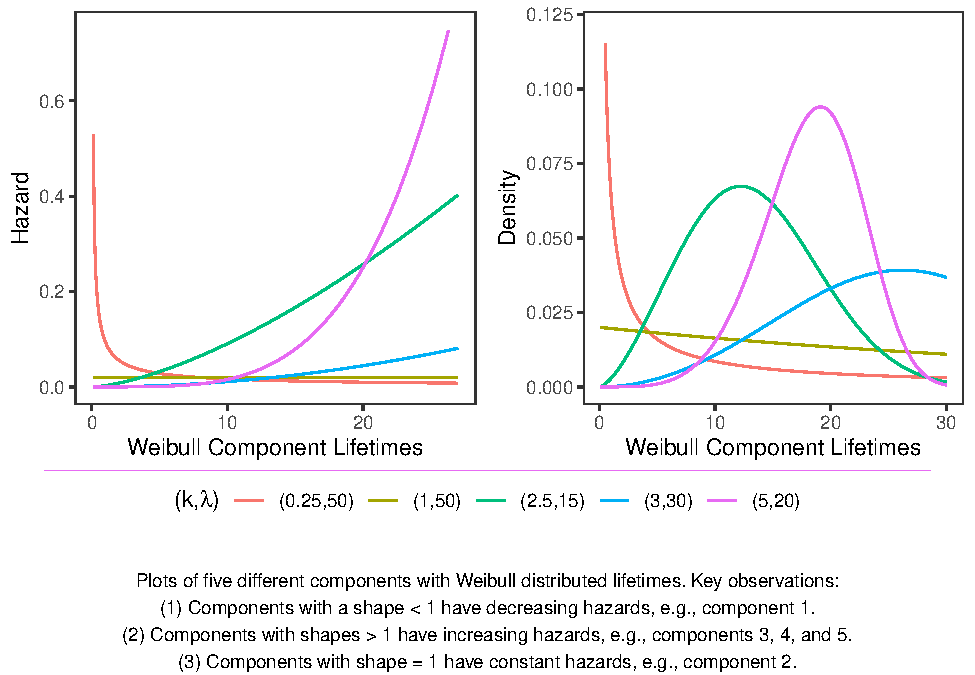
\includegraphics{wei_series_md_files/figure-latex/exp_weib_haz-1} 

}

\caption{Component lifetime plots}\label{fig:exp_weib_haz}
\end{figure}

The shape parameter \(k\) may be understood in the following way:

\begin{itemize}
\tightlist
\item
  If \(k < 1\), then the hazard function decreases with respect to
  system lifetime, which may occur if defective items fail early and are
  weeded out.
\item
  If \(k > 1\), then the hazard function is increases with respect to
  time, which may occur as a result of an aging process.
\item
  If \(k = 1\), then the failure rate is constant, which means it is
  exponentially distributed.
\end{itemize}

See Figure \ref{fig:exp_weib_haz} for plots of the hazard and pdf
functions of five different Weibull distributed components. We will use
these plots to illustrate the different shapes of the hazard and pdf
functions. The first component has a shape parameter \(k=0.25\), which
is less than 1, and so the hazard function decreases with respect to
time. The second component has a shape parameter \(k=1\), and so the
hazard function is constant. The third, fourth, and fifth components
have shape parameters \(k=2.5\), \(k=3\), and \(k=5\), respectively, and
so the hazard functions increase with respect to time.

The lifetime of the series system composed of \(m\) Weibull components
has a reliability function given by \begin{equation}
\label{eq:sys_weibull_reliability_function}
R(t;\boldsymbol{\theta}) = \exp\biggl\{-\sum_{j=1}^{m}\biggl(\frac{t}{\lambda_j}\biggr)^{k_j}\biggr\}.
\end{equation}

\begin{proof}
By Theorem \ref{thm:sys_reliability_function},
$$
R(t;\boldsymbol{\theta}) = \prod_{j=1}^{m} R_j(t;\lambda_j,k_j).
$$
Plugging in the Weibull component reliability functions obtains the result
\begin{align*}
R(t;\boldsymbol{\theta})
    &= \prod_{j=1}^{m} \exp\biggl\{-\biggl(\frac{t}{\lambda_j}\biggr)^{k_j}\biggr\}\\
    &= \exp\biggl\{-\sum_{j=1}^{m}\biggl(\frac{t}{\lambda_j}\biggr)^{k_j}\biggr\}.
\end{align*}
\end{proof}

The Weibull series system's hazard function is given by \begin{equation}
\label{eq:sys_weibull_failure_rate_function}
h(t;\boldsymbol{\theta}) =
    \sum_{j=1}^{m} \frac{k_j}{\lambda_j}\biggl(\frac{t}{\lambda_j}\biggr)^{k_j-1},
\end{equation} whose proof follows from Theorem
\ref{thm:sys_failure_rate}.

\begin{figure}

{\centering 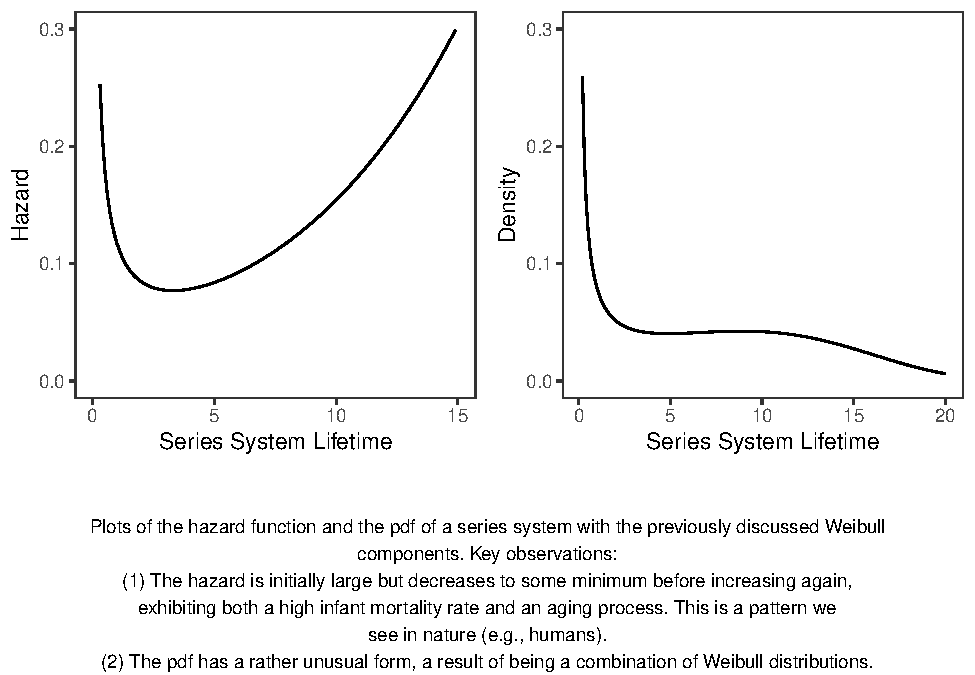
\includegraphics{wei_series_md_files/figure-latex/series_haz_pdf-1} 

}

\caption{System lifetime plots}\label{fig:series_haz_pdf}
\end{figure}

In Figure \ref{fig:series_haz_pdf}, we plot the hazard function and the
pdf of the Weibull series system with the component lifetime parameters
considered earlier, \begin{align*}
T_{i 1} &\sim \operatorname{WEI}(3,30)\\
T_{i 2} &\sim \operatorname{WEI}(2,50)\\
T_{i 3} &\sim \operatorname{WEI}(0.5,15)\\
T_{i 4} &\sim \operatorname{WEI}(5,20)\\
T_{i 5} &\sim \operatorname{WEI}(0.25,50)\\
\end{align*} for the \(i\)-th series system where \(i=1,\ldots,n\). By
Theorem \ref{thm:sys_lifetime}, the series system has a random lifetime
given by \[
T_i = \operatorname{min}\{T_{i 1},\ldots,T_{i 5}\}.
\] where \(\boldsymbol{\theta }= (k_1,\lambda_1,\ldots,k_5,\lambda_5)\).

The series system, due to being a mixture of Weibull components with
different shapes, has both a high infant mortality rate and an aging
process, which is reflected in the plot of the hazard function. The
hazard is initially high then decreases to some minimum before
increasing again. This is a pattern we see in nature, e.g., electronic
appliances may fail early due to defects, but those that survive the
initial period of high failure rate can be expected to last for a long
time before finally wearing out due to an aging process.

The pdf of the series system also appears to be multimodal, where the
modes correspond to the high infant mortality rate and the aging
process.

The pdf of the series system is given by \begin{equation}
\label{eq:sys_weibull_pdf}
f(t;\boldsymbol{\theta}) =
\biggl\{
    \sum_{j=1}^m \frac{k_j}{\lambda_j}\left(\frac{t}{\lambda_j}\right)^{k_j-1}
\biggr\}
\exp
\biggl\{
    -\sum_{j=1}^m \bigl(\frac{t}{\lambda_j}\bigr)^{k_j}
\biggr\}.
\end{equation}

\begin{proof}
By definition,
$$
f(t;\boldsymbol{\theta}) = h(t;\boldsymbol{\theta}) R(t;\boldsymbol{\theta}).
$$
Plugging in the failure rate and reliability functions given respectively by
Equations \eqref{eq:sys_weibull_reliability_function} and
\eqref{eq:sys_weibull_failure_rate_function} completes the proof.
\end{proof}

The conditional pmf of \(K_i\) given \(T_i\) is given by
\begin{equation}
\label{eq:weibull_pmf_k_given_s}
f(k;\boldsymbol{\theta}|t) = \frac{\frac{k_k}{\lambda_k}\bigl(\frac{t}{\lambda_k}\bigr)^{k_k-1}}
    {\sum_{j=1}^m \frac{k_j}{\lambda_j}\bigl(\frac{t}{\lambda_j}\bigr)^{k_j-1}}.
\end{equation}

\begin{proof}
By Theorem \ref{thm:f_given_s_form_2},
$$
f(k;\boldsymbol{\theta}|t) = \frac{h_k(t;\boldsymbol{\theta_k})}{\sum_{j=1}^m h_j(t;\boldsymbol{\theta_j})}
$$
where $h_1,\ldots,h_m$ are the failure rate functions of the $m$ Weibull
component lifetimes.
\end{proof}

The joint pdf of \(K_i\) and \(T_i\) is given by \begin{equation}
\label{eq:weibull_joint_k_s}
f(k,t;\boldsymbol{\theta}) = \frac{k_k}{\lambda_j}\biggl(\frac{t}{\lambda_k}\biggr)^{k_k-1}
\exp\biggl\{-\sum_{j=1}^{m}\biggl(\frac{t}{\lambda_j}\biggr)^{k_j}\biggr\}.
\end{equation}

\begin{proof}
Plugging in the conditional probability and the marginal probability given
respectively by Equations \eqref{eq:expo_prob_K_given_S} and
\eqref{eq:expo_sys_pdf} completes the proof.

By Theorem \ref{thm:f_k_and_t}, the joint pdf of $K_i$ and $T_i$ is given by
$$
f(k,t;\boldsymbol{\theta}) = h_k(t;\boldsymbol{\theta_k}) R_{T_i}(t;\boldsymbol{\theta})
$$
where $R_{T_i}(t;\boldsymbol{\theta})$ is given by Equation
\eqref{eq:sys_weibull_reliability_function} and $h_k$ is the failure rate
function of the $k$\textsuperscript{th} Weibull component.
\end{proof}

\hypertarget{weibull-likelihood-model-for-masked-data}{%
\subsection{Weibull Likelihood Model for Masked
Data}\label{weibull-likelihood-model-for-masked-data}}

In Section \ref{sec:like_model}, we discussed two separate kinds of
likelihood contributions, masked component cause of failure data (with
exact system failure times) and right-censored data. The likelihood
contribution of the \(i\)\textsuperscript{th} system is given by the
following theorem.

\begin{theorem}
Let $\delta_i$ be an indicator variable that is 1 if the
$i$\textsuperscript{th} system fails and 0 (right-censored) otherwise.
Then the likelihood contribution of the $i$\textsuperscript{th} system is given by
\begin{equation}
\label{eq:weibull_likelihood_contribution}
L_i(\boldsymbol{\theta}) =
\begin{cases}
    \exp\biggl\{-\sum_{j=1}^{m}\bigl(\frac{t_i}{\lambda_j}\bigr)^{k_j}\biggr\}
        \beta_i \sum_{j \in c_i} \frac{k_j}{\lambda_j}\bigl(\frac{t_i}{\lambda_j}\bigr)^{k_j-1}
    & \text{if } \delta_i = 1,\\
    \exp\bigl\{-\sum_{j=1}^{m}\bigl(\frac{t_i}{\lambda_j}\bigr)^{k_j}\biggr\} & \text{if } \delta_i = 0.
\end{cases}
\end{equation}
\end{theorem}
\begin{proof}
By Theorem \ref{thm:likelihood_contribution}, the likelihood contribution of the
$i$-th system is given by
$$
L_i(\boldsymbol{\theta}) =
\begin{cases}
    R_{T_i}(s_i;\boldsymbol{\theta})                      &\text{ if } \delta_i = 0\\
    \beta_i R_{T_i}(s_i;\boldsymbol{\theta})
        \sum_{j\in c_i} h_j(s_i;\boldsymbol{\theta_j})   &\text{ if } \delta_i = 1.
\end{cases}
$$
By Equation \eqref{eq:sys_weibull_reliability_function}, the system reliability
function $R_{T_i}$ is given by
$$
R_{T_i}(t_i;\boldsymbol{\theta}) = \exp\biggl\{-\sum_{j=1}^{m}\biggl(\frac{t_i}{\lambda_j}\biggr)^{k_j}\biggr\}.
$$
and by Equation \eqref{eq:weibull_haz}, the Weibull component hazard function $h_j$ is
given by
$$
h_j(t_i;\boldsymbol{\theta_j}) = \frac{k_j}{\lambda_j}\biggl(\frac{t_i}{\lambda_j}\biggr)^{k_j-1}.
$$
Plugging these into the likelihood contribution function obtains the result.
\end{proof}

Taking the log of the likelihood contribution function obtains the
following result.

\begin{corollary}
The log-likelihood contribution of the $i$-th system is given by
\begin{equation}
\label{eq:weibull_log_likelihood_contribution}
\ell_i(\boldsymbol{\theta}) =
-\sum_{j=1}^{m}\biggl(\frac{t_i}{\lambda_j}\biggr)^{k_j} +
    \delta_i \log \!\Biggl(    
        \sum_{j \in c_i} \frac{k_j}{\lambda_j}\biggl(\frac{t_i}{\lambda_j}\biggr)^{k_j-1}
    \Biggr)
\end{equation}
where we drop any terms that do not depend on $\boldsymbol{\theta}$ since they do not
affect the MLE.
\end{corollary}

Since the systems are independent, the log-likelihood of the entire
sample of \(n\) observations is given by \begin{equation}
\label{eq:weibull_log_likelihood}
\ell(\boldsymbol{\theta}) = \sum_{i=1}^n \ell_i(\boldsymbol{\theta}).
\end{equation}

\hypertarget{maximum-likelihood-estimation}{%
\subsection{Maximum likelihood
estimation}\label{maximum-likelihood-estimation}}

We may find an MLE by solving the maximum likelihood equation
\eqref{eq:mle_eq}, i.e., a point
\(\boldsymbol{\hat\theta} = (\hat{k}_1,\hat{\lambda}_1,\ldots,\hat{k}_m,\hat{\lambda}_m)\)
satisfying
\(\nabla_{\theta} \ell(\boldsymbol{\hat\theta}) = \boldsymbol{0}\),
where \(\nabla_{\boldsymbol{\theta}}\) is the gradient of the
log-likelihood function with respect to \(\boldsymbol{\theta}\),
otherwise known as the score.

To solve these ML equations, we use the Newton-Raphson method described
in Section \ref{sec:iterative}. In order to use the Newton-Raphson
method, we need to compute the gradient and Hessian of the
log-likelihood function.

We analytically derive the gradient of the log-likelihood function
(score), since it is useful to have for the Newton-Raphson method, but
we do not do the same for the Hessian of the log-likelihood for the
following reasons:

\begin{enumerate}
\def\labelenumi{\arabic{enumi}.}
\item
  The Hessian is not necessarily needed since we often use some faster
  method to approximate the Hessian, e.g., the BFGS method. Technically,
  we could also numerically approximate the gradient too, but the
  gradient is much easier to derive than the Hessian, and moreover,
  knowing the score precisely also enables us to more accurately
  approximate the Hessian by taking the Jacobian of the gradient.
\item
  The Hessian is more difficult to derive than the score, and so it is
  more likely that we will make a mistake when deriving the Hessian.
\end{enumerate}

The following theorem derives the score function.

\begin{theorem}
\label{thm:weibull_score}
The score function of the log-likelihood contribution of the $i$-th Weibull series
system is given by
\begin{equation}
\label{eq:weibull_score}
\nabla \ell_i(\boldsymbol{\theta}) = \biggl(
    \frac{\partial \ell_i(\boldsymbol{\theta})}{\partial k_1},
    \frac{\partial \ell_i(\boldsymbol{\theta})}{\partial \lambda_1},
    \cdots, 
    \frac{\partial \ell_i(\boldsymbol{\theta})}{\partial k_m},
    \frac{\partial \ell_i(\boldsymbol{\theta})}{\partial \lambda_m} \biggr)',
\end{equation}
where
\begin{equation}
\frac{\partial \ell_i(\boldsymbol{\theta})}{\partial k_r} = 
    -\biggl(\frac{t_i}{\lambda_r}\biggr)^{k_r}    
        \!\!\log\biggl(\frac{t_i}{\lambda_r}\biggr) +
        \frac{\frac{1}{t_i} \bigl(\frac{t_i}{\lambda_r}\bigr)^{k_r}
            \bigl(1+ k_r \log\bigl(\frac{t_i}{\lambda_r}\bigr)\bigr)}
            {\sum_{j \in c_i} \frac{k_j}{\lambda_j}\bigl(\frac{t_i}{\lambda_j}\bigr)^{k_j-1}}
        1_{\delta_i = 1 \land r \in c_i}
\end{equation}
and 
\begin{equation}
\frac{\partial \ell_i(\boldsymbol{\theta})}{\partial \lambda_r} = 
    \frac{k_r}{\lambda_r} \biggl(\frac{t_i}{\lambda_r}\biggr)^{k_r} -
    \frac{
        \bigl(\frac{k_r}{\lambda_r}\bigr)^2 \bigl(\frac{t_i}{\lambda_r}\bigr)^{k_r - 1}
    }
    {
        \sum_{j \in c_i} \frac{k_j}{\lambda_j}\bigl(\frac{t_i}{\lambda_j}\bigr)^{k_j-1}
    }
    1_{\delta_i = 1 \land r \in c_i}
\end{equation}
\end{theorem}

\begin{proof}
The log-likelihood contribution for the i-th observation is given by Equation \eqref{eq:weibull_log_likelihood_contribution}:
$$
\ell_i = -\sum_{j=1}^m \biggl(\frac{t_i}{\lambda_j}\biggr)^{k_j} +
    \delta_i \log \Biggl(\sum_{j \in c_i} \frac{k_j}{\lambda_j} \biggl(\frac{t_i}{\lambda_j}\biggr)^{k_j - 1} \Biggr).
$$

\textbf{Shape parameters: $\partial \ell_i / \partial k_r$}

Proof steps here.

\textbf{Scale parameters: $\partial \ell_i / \partial \lambda_r$}
We want to find the derivative of $\ell_i$ with respect to $\lambda_r$. 
The derivative of the sum of functions is the sum of the derivatives, so we can
differentiate each term in the sum separately. 

First, we differentiate
$$
    -\sum_{j=1}^m (t_i/\lambda_j)^{k_j}
$$
with respect to $\lambda_r$. The derivative of this term with respect to
$\lambda_r$ is zero for all $j$ not equal to $r$, and for $j = r$, we have
$-(t_i/\lambda_r)^{k_r}$. The derivative of this term with respect to $\lambda_r$ is
$$
\frac{k_r}{\lambda_r} \biggl(\frac{t_i}{\lambda_r}\biggr)^{k_r}.
$$

Second, we differentiate
$$
\delta_i \log\Biggl(\sum_{j \in c_i} \frac{k_j}{\lambda_j} \biggl(\frac{t_i}{\lambda_j}\biggr)^{k_j - 1}\Biggr)
$$
with respect to $\lambda_r$.
The derivative of the logarithm of a function is the derivative of the function
divided by the function itself.
The function inside the logarithm is
$$
\sum_{j \in c_i} \frac{k_j}{\lambda_j} \left(\frac{t_i}{\lambda_j}\right)^{k_j - 1}. 
$$
The derivative of this function with respect to $\lambda_r$ is zero for all $j$ not
in $c_i$ or not equal to $r$, and for $j = r$ in $c_i$, we have
$$
\frac{k_r}{\lambda_r} \left(\frac{t_i}{\lambda_r}\right)^{k_r - 1}. 
$$
The derivative of this term with respect to $\lambda_r$ is
$$
\biggl(\frac{k_r}{\lambda_r}\biggr)^2 \biggl(\frac{t_i}{\lambda_r}\biggr)^{k_r - 1}.
$$
So, the derivative of the second term is
$$
\delta_i \frac{\bigl(\frac{k_r}{\lambda_r}\bigr)^2 \bigl(\frac{t_i}{\lambda_r}\bigr)^{k_r - 1} }
{\sum_{j \in c_i} \frac{k_j}{\lambda_j}\bigl(\frac{t_i}{\lambda_j}\bigr)^{k_j-1}}
$$
if $r$ in $c_i$ and zero otherwise.

Adding the derivatives of the first and second terms, we get the partial derivative
of $\ell_i$ with respect to $\lambda_r$,
$$
\frac{\partial \ell_i(\boldsymbol{\theta})}{\partial \lambda_r} = 
    \frac{k_r}{\lambda_r} \biggl(\frac{t_i}{\lambda_r}\biggr)^{k_r} -
    \delta_i \frac{
        \bigl(\frac{k_r}{\lambda_r}\bigr)^2 \bigl(\frac{t_i}{\lambda_r}\bigr)^{k_r - 1}
    }
    {
        \sum_{j \in c_i} \frac{k_j}{\lambda_j}\bigl(\frac{t_i}{\lambda_j}\bigr)^{k_j-1}
    },
$$
if $r \in c_i$ and zero otherwise.
This is the partial derivative of $\ell_i$ with respect to $\lambda_r$.
\end{proof}

These results follow from taking the partial derivatives of the
log-likelihood contribution of the \(i\)-th system given by Equation
\eqref{eq:weibull_likelihood_contribution}. The proof is omitted for
brevity, but the results have been verified by using a very precise
numerical approximation of the gradient and verifying equality with the
analytical gradient on different data sets and parameter values.

By the linearity of differentiation, the gradient of a sum of functions
is the same of their gradients, and so the score function of the entire
sample is given by \begin{equation}
\label{eq:weibull_series_score}
\nabla \ell(\boldsymbol{\theta}) = \sum_{i=1}^n \nabla \ell_i(\boldsymbol{\theta}).
\end{equation}

\hypertarget{simulation-study-weibull-series-system}{%
\section{Simulation study: Weibull series
system}\label{simulation-study-weibull-series-system}}

In the real world, systems are quite complex:

\begin{enumerate}
\def\labelenumi{\arabic{enumi}.}
\item
  They are not perfect series systems.
\item
  The components in a system are not independent.
\item
  The lifetimes of the systems (in the population) are not precisely
  modeled by any known probability distributions.
\item
  The components may depend on many other unobserved factors.
\end{enumerate}

With these caveats in mind, we model the data as coming from a Weibull
series system of \(m = 5\) components, and other factors, like ambient
temperature, are either negligible (on the distribution of component
lifetimes) or are more or less constant. Then, our task is to use our
likelihood model to find the best fit using maximum likelihood
estimation.

\hypertarget{bernoulli-candidate-set-model}{%
\subsection{Bernoulli candidate set
model}\label{bernoulli-candidate-set-model}}

In our simulation study, we must generate data that satisfies the
masking conditions. In other words, we must generate data that satisfies
the conditions described in Section \ref{sec:candmod}.

There are many ways to satisfying the masking conditions. We choose the
simplest method, which we call the \emph{Bernoulli candidate set model}.
In this model, each non-failed component is included in the candidate
set with a fixed probability \(p\), independently of all other
components and independently of \(\boldsymbol{\theta}\), and the failed
component is always included in the candidate set.

\hypertarget{identifiability}{%
\subsection{Identifiability}\label{identifiability}}

When estimating the parameters of latent components, we must be careful
to ensure that the parameters are identifiable. In other words, we must
ensure that the likelihood function is maximized at a unique point. If
the likelihood function is not maximized at a unique point, then the MLE
is not unique, and a lot of the theory we have developed so far breaks
down.

One way in which this problem may arise is if the data is not
informative enough. For example, if we have a series system with \(m\)
components, and in the sample component \(1\) is in the candidate set if
and only if component \(2\) is in candidate set, then we do not have
enough information to estimate the parameters of component \(1\) and
component \(2\) separately. In this case, we could combine these two
components into one component, and then we would have \(m-1\) components
to estimate instead. We lagely avoid this problem by using the Bernoulli
candidate set model, but sometimes it may still arise by chance.

\hypertarget{sec:opt_rescale}{%
\subsection{Optimization issue: parameter
rescaling}\label{sec:opt_rescale}}

When the parameters under investigation span different orders of
magnitude, parameter rescaling can significantly improve the performance
and reliability of optimization algorithms.

Parameter rescaling gives an optimizer a sense of the typical size of
each parameter, enabling it to adjust its steps accordingly. This is
crucial in scenarios like ours, where shape and scale parametes are a
few orders of magnitude apart. Without rescaling, the optimization
routine may struggle, taking numerous small steps for larger parameters
and overshooting for smaller ones.

In the \texttt{optim} algorithm in the R package \texttt{stats}, we
achieve this result by assigning a \texttt{parscale} vector in line with
the parameter magnitudes. It does not matter what the values of the
\texttt{parscale} vector are, only their relative magnitudes. It does
not need to be very precise, but since we are doing a simulation study,
we know the true parameter values and can use that information to scale
them appropriately. We found that this allowed for convergence to MLEs
more quickly and reliably.

\hypertarget{simulation-study-design}{%
\subsection{Simulation study design}\label{simulation-study-design}}

In order to make the simulation study representative of real-world
scenarios, we must choose parameter values that are realistic. We base
our parameters on the data from {[}3{]}, which includes a study of the
reliability of a series system with three Weibull components
parameterized by \(\boldsymbol{\theta}\) with shape parameters given by
\[
    k_1 = 1.2576,
    k_2 = 1.1635,
    k_3 = 1.1308,
\] and scale parameters given by \[
    \lambda_1 = 994.3661,
    \lambda_2 = 908.9458,
    \lambda_3 = 840.1141.
\]

In our Bernoulli candidate set model, we estimated that with around
probability \(p = 0.215\) for including each non-failed component in the
candidate set and with a right-censoring time of \(\tau = \infty\), we
seem to reproduce their reported data.

Our approach is to extend this to a five component Weibull series
system, and then we vary the sample size \(n\), the Bernoulli masking
probability \(p\) of including each non-failed component in the
candidate set, and the right-censoring time \(\tau\). We then analyze
the performance of the MLE under these various scenarios.

The true parameter value \(\boldsymbol{\theta}\) of the five component
Weibull series system has shape parameters given by \[
    k_1 = 1.2576,
    k_2 = 1.1635,
    k_3 = 1.1308,
    k_4 = 1.1802,
    k_5 = 1.3311
\] and scale parameters given by \[
    \lambda_1 = 994.3661,
    \lambda_2 = 908.9458,
    \lambda_3 = 840.1141,
    \lambda_4 = 940.1141,
    \lambda_5 = 836.1123.
\]

Here is an outline of the simulation study analysis:

\begin{enumerate}
\def\labelenumi{\arabic{enumi}.}
\item
  Set up simulation parameters for various scenarios of interest, such
  as generating data to examine the relationship between bias and
  masking probability for different sample sizes and right-censoring
  times.
\item
  Generate \(R\) data sets for each scenario (some combination of \(n\),
  \(p\), and \(\tau\)).
\item
  Estimate the parameters for each data set, giving us \(R\) estimates
  of the parameters. We use these data sets as an empirical estimate of
  the sampling distribution of the MLE for each scenario.
\item
  Using the empirical sampling distribution of the MLE, estimate various
  performance measures of the MLE, like bias, variance, MSE, and
  coverage probability for each scenario.
\item
  Analyze and visualize the results, e.g., by plotting the bias,
  variance, MSE, and coverage probability as a function of \(n\) for
  different combinations of \(p\) and \(\tau\).

  We then interpret the results and discuss the performance of the MLE
  estimator under various conditions. We expect that as
  \(n \to \infty\), the bias and MSE will go to \(0\) and the coverage
  probability will go to \(0.95\) (when constructing \(95\%\) confidence
  intervals). Of course, we do not expect these results to hold for
  finite \(n\), but we would like to see how the bias, MSE, and coverage
  probability change as we vary \(n\), \(p\), and \(\tau\).
\end{enumerate}

For how we generate a scenario, see Appendix A.

\hypertarget{verification}{%
\subsubsection{Verification}\label{verification}}

To verify that our likelihood model is correct, we load the Table 2 data
from {[}3{]} and fit the Weibull series model to the data to see if we
can recover the MLE they reported. When we fit the Weibull series model
to this data by maximizing the likelihood function, we obtain the
following fit for the shape and scale parameters given respectively by
\[
    \hat{k}_1 = 1.2576,
    \hat{k}_2 = 1.1635,
    \hat{k}_3 = 1.1308,
\] and \[
    \hat{\lambda}_1 = 994.3661,
    \hat{\lambda}_2 = 908.9458,
    \hat{\lambda}_3 = 840.1141,
\] which is in agreement with the MLE they reported. Satisfied that our
likelihood model is correct, we proceed with the simulation study.

\hypertarget{sec:acc_prec}{%
\subsection{Analysis of the MLE}\label{sec:acc_prec}}

The primary purpose of the simulation study is to anlyze the performance
of the MLE under different scenarios. We will compute the bias,
variance, MSE, confidence interval widths, and coverage proababilities
for confidence intervals with respect to a range of scenarios to
quantify the performance of the MLE under different circumstances.

\hypertarget{bias}{%
\subsubsection{Bias}\label{bias}}

A measure of the accuracy of \(\boldsymbol{\hat\theta}\) is the bias,
which is defined as \[
\operatorname{b}(\boldsymbol{\hat\theta}) = E(\boldsymbol{\hat\theta}) - \boldsymbol{\theta}.
\] We cannot analytically derive the bias, so we estimate the bias using
the empirical sampling distribution, \[
\hat{\operatorname{b}}(\boldsymbol{\hat\theta}) =
    E_{\hat{\boldsymbol{\theta}} \sim \text{data}}(\boldsymbol{\hat\theta}) - \boldsymbol{\theta}.
\]

\hypertarget{scenario-absolute-bias-vs.-sample-size-with-a-masking-probability-but-no-right-censoring}{%
\subparagraph*{Scenario: Absolute bias vs.~sample size with a masking
probability but no
right-censoring}\label{scenario-absolute-bias-vs.-sample-size-with-a-masking-probability-but-no-right-censoring}}
\addcontentsline{toc}{subparagraph}{Scenario: Absolute bias vs.~sample
size with a masking probability but no right-censoring}

In this scenario, we want to see the bias of the MLE as a function of
the sample size \(n\) from \(n = 30\) to \(n = 800\) for a fixed masking
probability \(p = 0.2\) and no right-censoring \((\tau = \infty)\).
Recall that the masking probability is the probability of including each
non-failed component.

\begin{figure}

{\centering 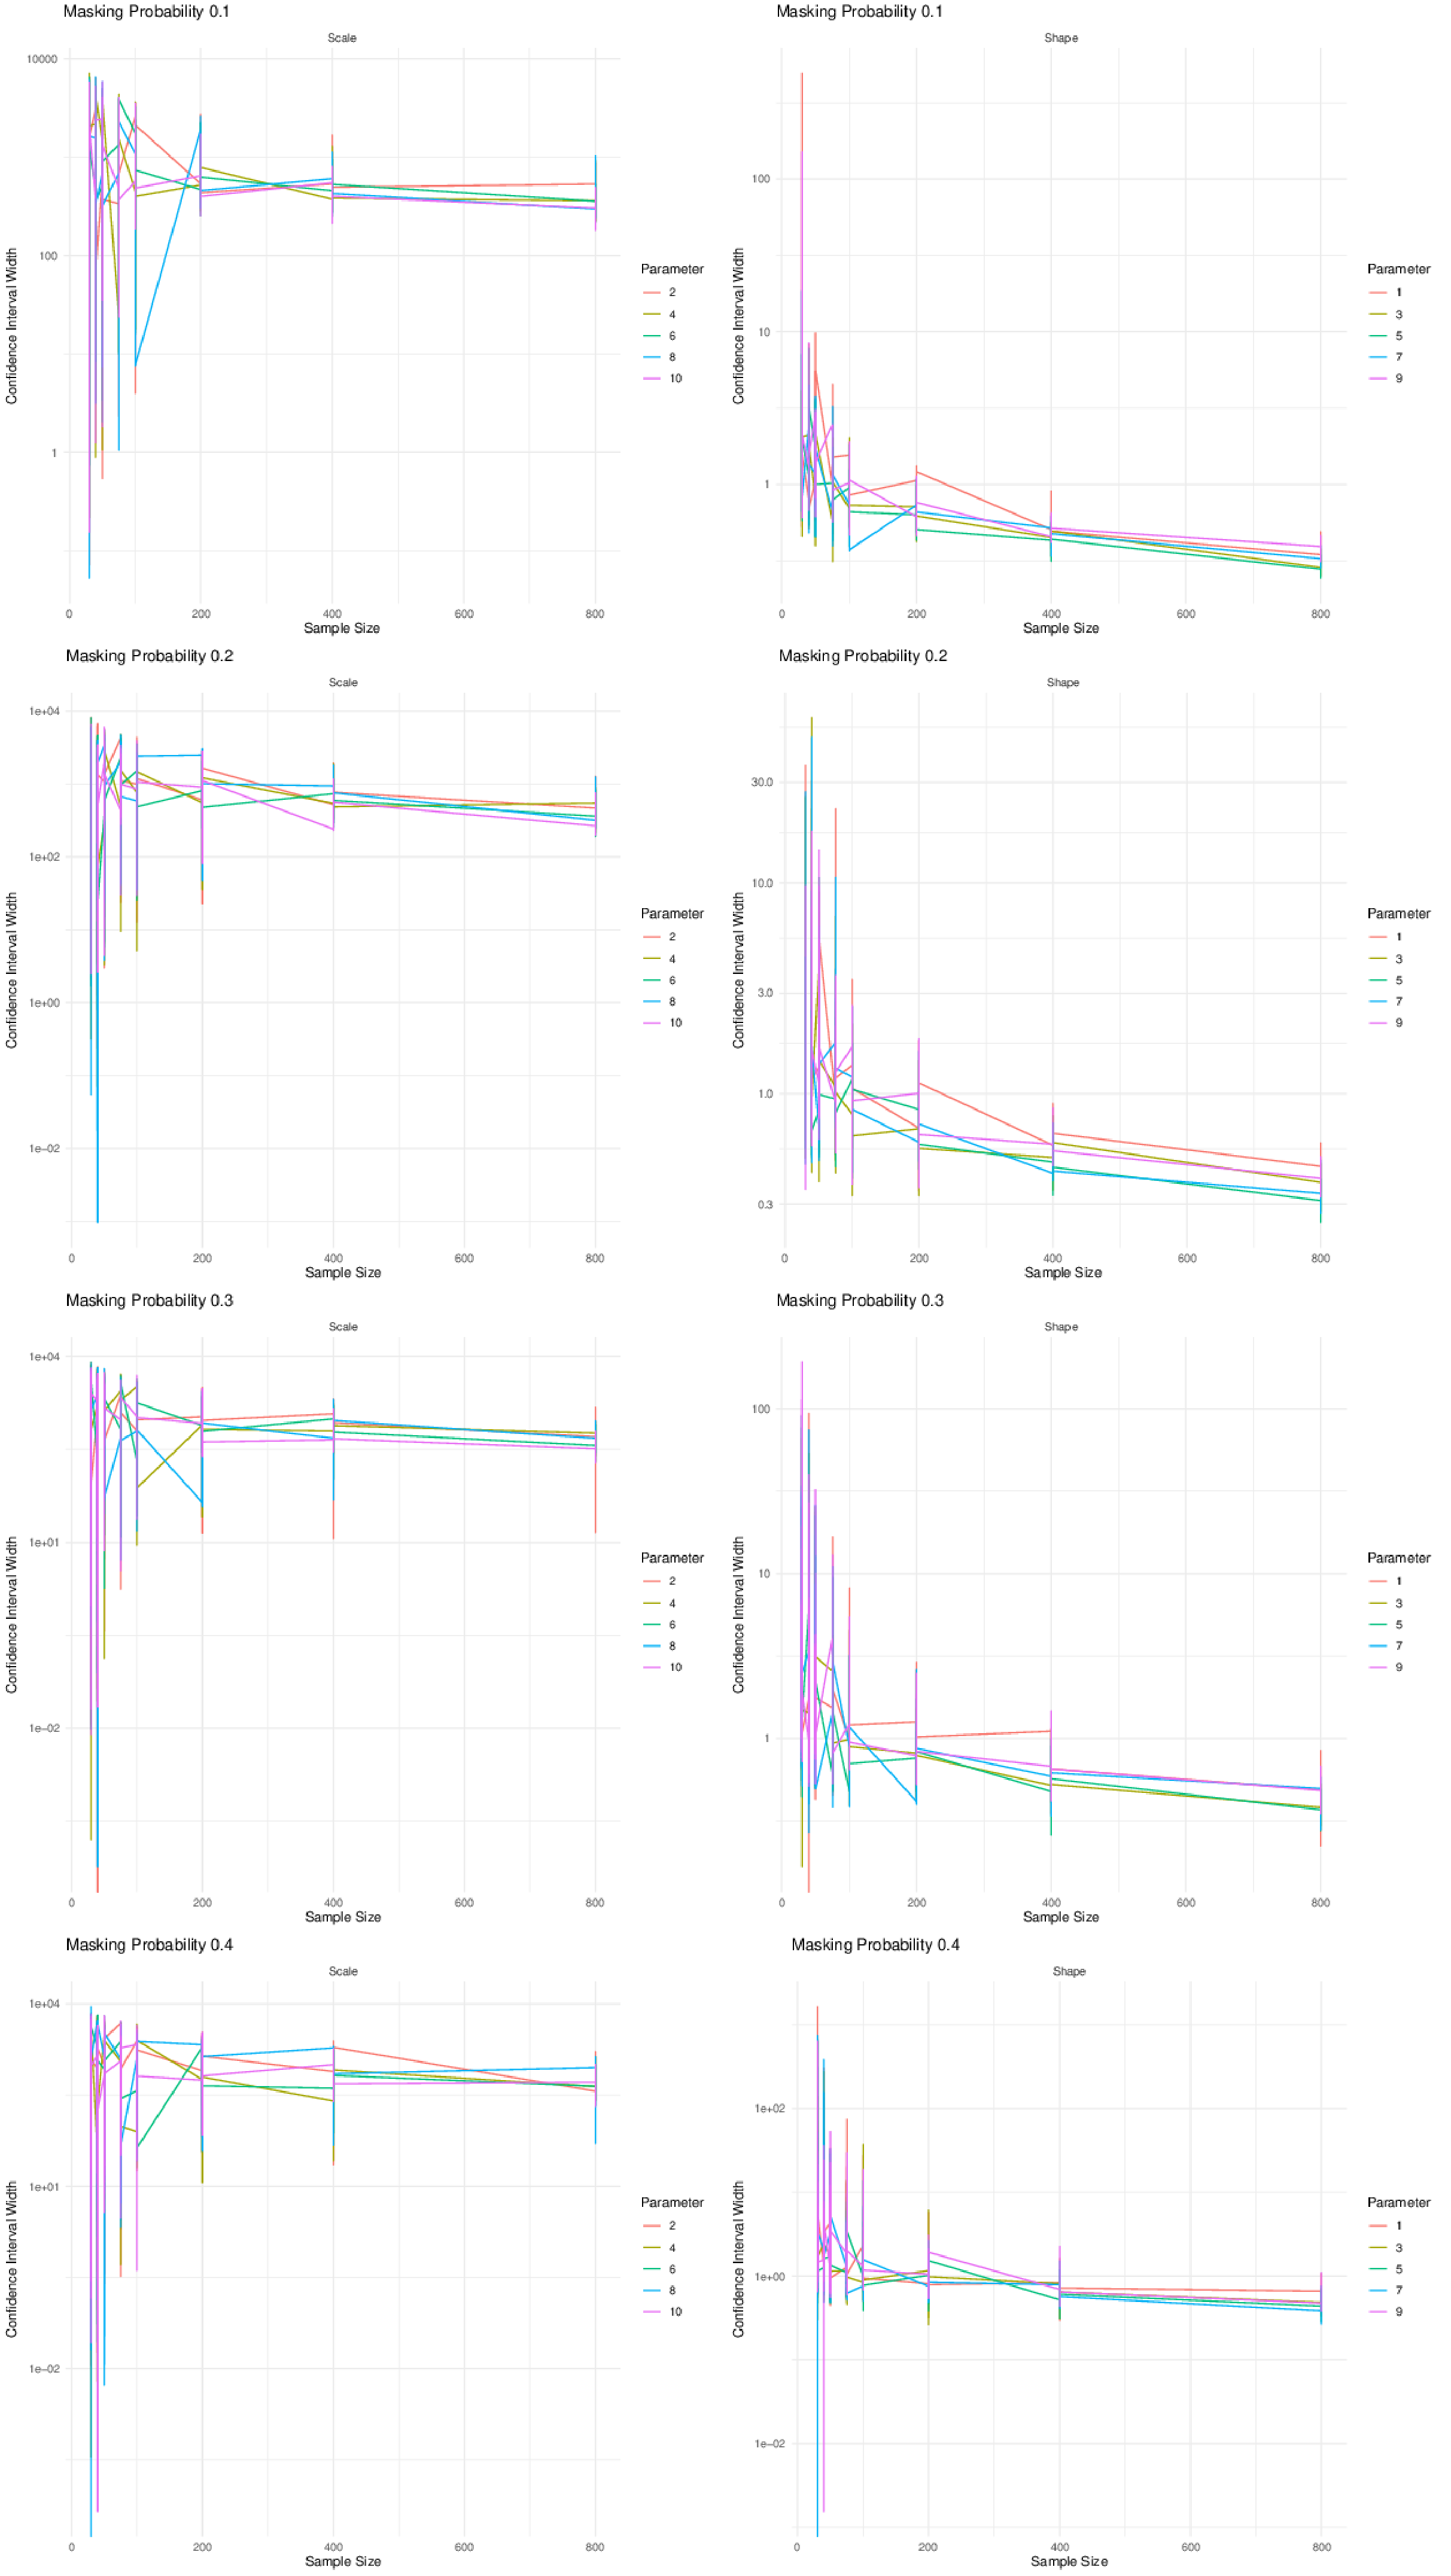
\includegraphics{image/plot-p-0.2-bias-vs-sample-size} 

}

\caption{Bias vs. sample size (masking probability 0.2)}\label{fig:plot-bias-p-0.2-vs-sample-size}
\end{figure}

In Figure \ref{fig:plot-bias-p-0.2-vs-sample-size}, we plot the absolute
bias \(|\operatorname{bias}(\hat\theta)|\) on a log scale against the
sample size. However, because the absolute bias is quite large for small
sample sizes and small for large sample sizes, we use a log scale.
Furthermore, we show the absolute bias for the shape and scale
parameters separately, since the scale parameters are much larger than
the shape parameters.

Here are some important observations Figure
\ref{fig:plot-bias-p-0.2-vs-sample-size} reveals:

\begin{enumerate}
\def\labelenumi{\arabic{enumi}.}
\item
  For both shape and scale parameters, we see that the absolute bias
  seems to be decreasing to zero as the sample size increases. This is
  not surprising since we expect the MLE to be consistent, i.e.,
  \(\boldsymbol{\hat\theta}\) converges in probability to
  \(\boldsymbol{\theta}\) as the sample size increases to infinity.
  Still, it is reassuring to see that the bias seems to be behaving as
  expected.
\item
  For the shape parameters, which are small (the shape parameters have
  true values a little larger than 1), the bias is relatively large for
  sample sizes up to \(100\).
\item
  For the scale parameters, which are quite large (the scale parameters
  have true values around 1000). Like with the shape parameters, the
  bias is relatively large for sample sizes up to \(100\), but seems to
  stabilize and reach relatively small values after that.
\end{enumerate}

\hypertarget{scenario-bias-vs.-sample-size-and-masking-probability-and-no-right-censoring}{%
\subparagraph*{Scenario: Bias vs.~sample size and masking probability
and no
right-censoring}\label{scenario-bias-vs.-sample-size-and-masking-probability-and-no-right-censoring}}
\addcontentsline{toc}{subparagraph}{Scenario: Bias vs.~sample size and
masking probability and no right-censoring}

Now, we take a larger view and plot the bias (without taking its
absolute value as we had done previously) against the masking
probabilities \(p = 0\) (no masking) to \(p = 0.4\) (significant
masking) for sample sizes 100, 400, and 800.

For the shape parameters, at a sample of size 100, we see significant
bias and we also see that it is very sensitive to the masking
probability. See Figure
\ref{fig:plot-bias-shapes-vs-p-sample-size-100-400-800}. However, for
sample sizes of 400 and 800, the bias is relatively small and unaffected
by the masking probability.

\begin{figure}

{\centering 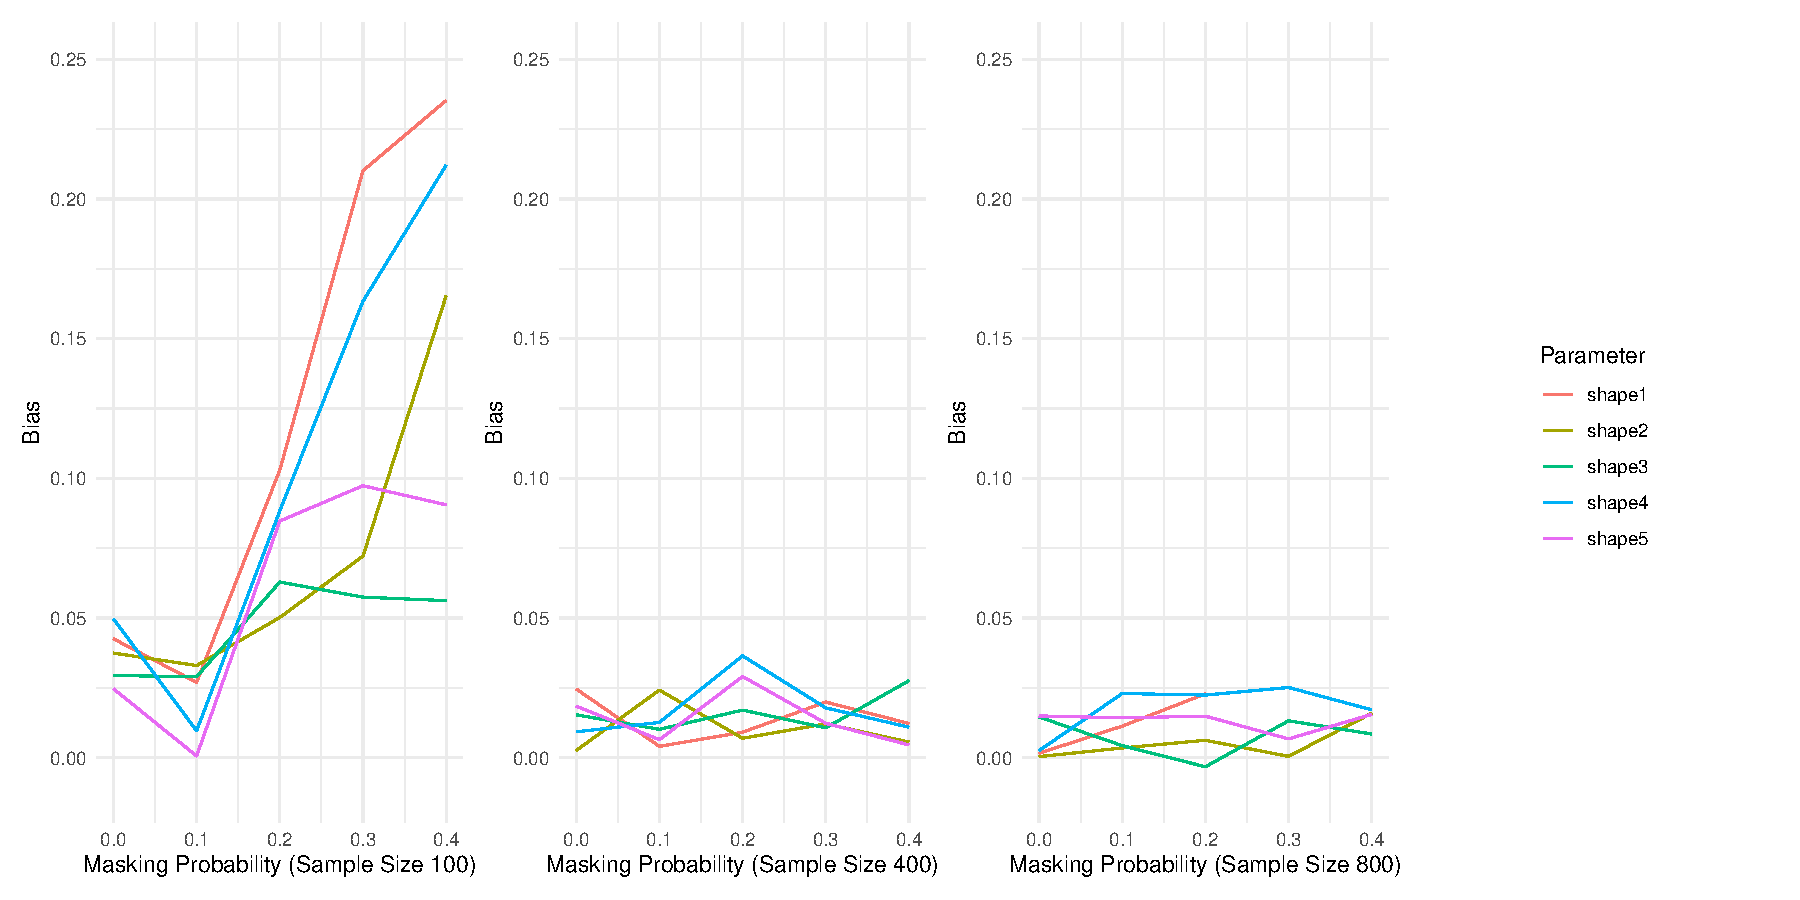
\includegraphics{image/plot-bias-shapes-p-vs-sample-size-100-400-800} 

}

\caption{Shape Bias vs. masking probability for sample sizes 100, 400, and 800}\label{fig:plot-bias-shapes-vs-p-sample-size-100-400-800}
\end{figure}

For the scale parameters, a similar pattern emerges, although we see
that even for sample size 400, there is evidence that the bias is still
affected by the masking probability. See Figure
\ref{fig:plot-bias-scales-vs-p-sample-size-100-400-800}.

The smallest bias, as expected, occurs for sample sizes of \(800\). The
bias for \(\lambda_1\) (scale parameter 1) at the masking probability
\(0.3\) is an interesting case, since it jumps up at that point for some
reason. We used only \(R = 100\) replications, so it is plausible it
would decrease with more replications. Regardless, the overall trend is
that the bias decreases as the sample size increases, and its dependence
on the masking probability is relatively small with sufficiently large
sample sizes.

\begin{figure}

{\centering 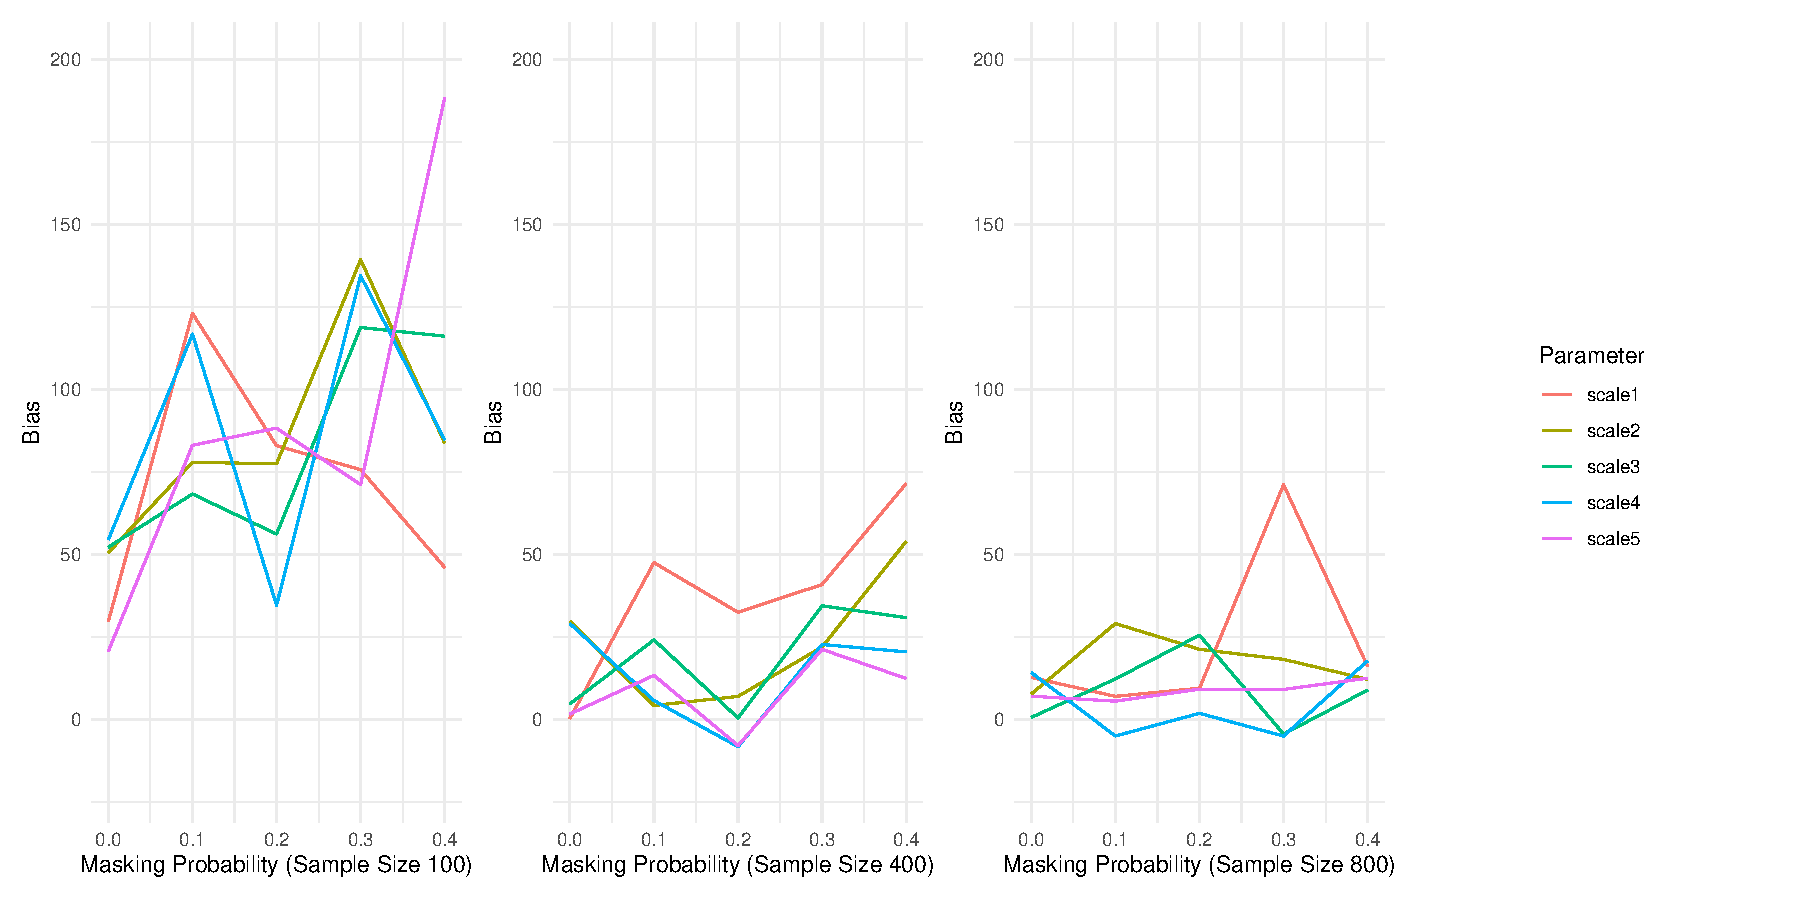
\includegraphics{image/plot-bias-scales-p-vs-sample-size-100-400-800} 

}

\caption{Scale Bias vs. masking probability for sample sizes 100, 400, and 800}\label{fig:plot-bias-scales-vs-p-sample-size-100-400-800}
\end{figure}

\hypertarget{scenario-bias-vs.-right-censoring-time-and-sample-size-with-a-fixed-masking-probability}{%
\paragraph*{Scenario: Bias vs.~right-censoring time and sample size with
a fixed masking
probability}\label{scenario-bias-vs.-right-censoring-time-and-sample-size-with-a-fixed-masking-probability}}
\addcontentsline{toc}{paragraph}{Scenario: Bias vs.~right-censoring time
and sample size with a fixed masking probability}

In this scenario, we want to isolate the effect of the right-censoring
time \(\tau\) on the bias. We fix the masking probability to
\(p = 0.215\), in line with the masking probability we estimate for the
Table 2 data set in {[}3{]}.

We plot the bias against the right-censoring time for sample sizes 50,
150, and 300. See Figure
\ref{fig:plot-bias-tau-vs-sample-size-50-150-300}. On the \(x\)-axis, we
report the right-censoring time as a quantile of the Weibull series
distribution so that we can more clearly see the effect of the
right-censoring on the bias, e.g., the \(50\%\) quantile is the time at
which \(50\%\) of the systems are expected to fail.

\begin{figure}

{\centering 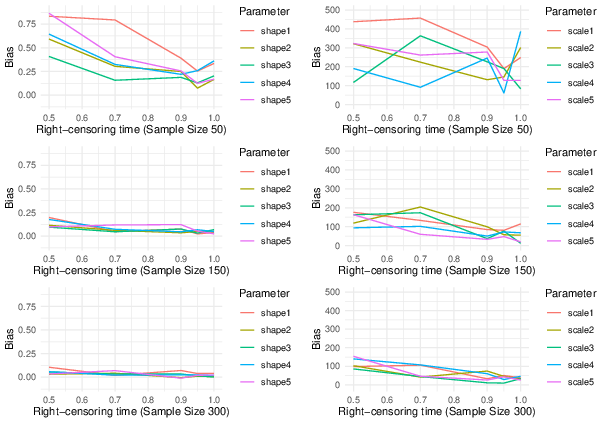
\includegraphics{image/plot-bias-tau-vs-sample-size-50-150-300} 

}

\caption{Bias vs. right-censoring time and sample sizes 50, 150, and 300}\label{fig:plot-bias-tau-vs-sample-size-50-150-300}
\end{figure}

A few observations about Figure
\ref{fig:plot-bias-tau-vs-sample-size-50-150-300}:

\begin{enumerate}
\def\labelenumi{\arabic{enumi}.}
\item
  The bias decreases as the right-censoring time increases. This is
  expected since we have more information about the system when the
  right-censoring time is larger.
\item
  The bias decreases as the sample size increases, which is also
  expected since we have more information about the system when the
  sample size is larger.
\item
  The bias is relatively small for sample sizes 150 and 300, but for
  sample size 50, the bias is quite large, particularly for the shape
  parameters. This is not surprising since the sample size is quite
  small, and so we do not expect the MLE to be very accurate.
\end{enumerate}

\hypertarget{sec:coverage_prob}{%
\subsubsection{Coverage probability}\label{sec:coverage_prob}}

We will use the inverse of the observed Fisher information matrix (FIM),
which was defined in Section \ref{sec:mle_properties}, to construct
\(95\%\)-confidence intervals for \(\boldsymbol{\theta}\) to compute the
coverage probability of the MLE for each scenario. A confidence interval
is said to be \emph{well-calibrated} if the coverage probability is
close to the nominal level, \(95\%\).

We want the coverage probability to be close to the nominal level,
\(95\%\), because if the coverage probability is too low, then we will
be too confident in the precision and accuracy of the MLE, and if the
coverage probability is too high, then we will not be confident enough
in the precision and accuracy of the MLE.

To estimate the coverage probability, we use the following procedure:

\begin{enumerate}
\def\labelenumi{\arabic{enumi}.}
\item
  For a given scenario (say, sample size and masking probability), we
  generate \(R = 100\) data sets.
\item
  We find an MLE for each of \(R\) data sets.
\item
  We compute the \(95\%\)-confidence interval for each MLE using the
  inverse of the observed FIM.
\item
  We compute the coverage probability by calculating the proportion of
  times the true parameter values were contained in computed the
  \(95\%\)-confidence interval.
\end{enumerate}

\hypertarget{scenario-coverage-probability-vs.-sample-size-with-a-fixed-masking-probability-and-no-right-censoring}{%
\paragraph*{Scenario: Coverage probability vs.~sample size with a fixed
masking probability and no
right-censoring}\label{scenario-coverage-probability-vs.-sample-size-with-a-fixed-masking-probability-and-no-right-censoring}}
\addcontentsline{toc}{paragraph}{Scenario: Coverage probability
vs.~sample size with a fixed masking probability and no right-censoring}

We want to isolate the effect of the coverage probability as a function
of the sample size \(n\). We fix the masking probability to \(p = 0.2\)
and without right-censoring \((\tau = \infty)\) and vary the sample size
from \(n = 30\) to \(n = 800\). See Figure
\ref{fig:plot-coverage-p-three-vs-sample-size}.

\begin{figure}

{\centering 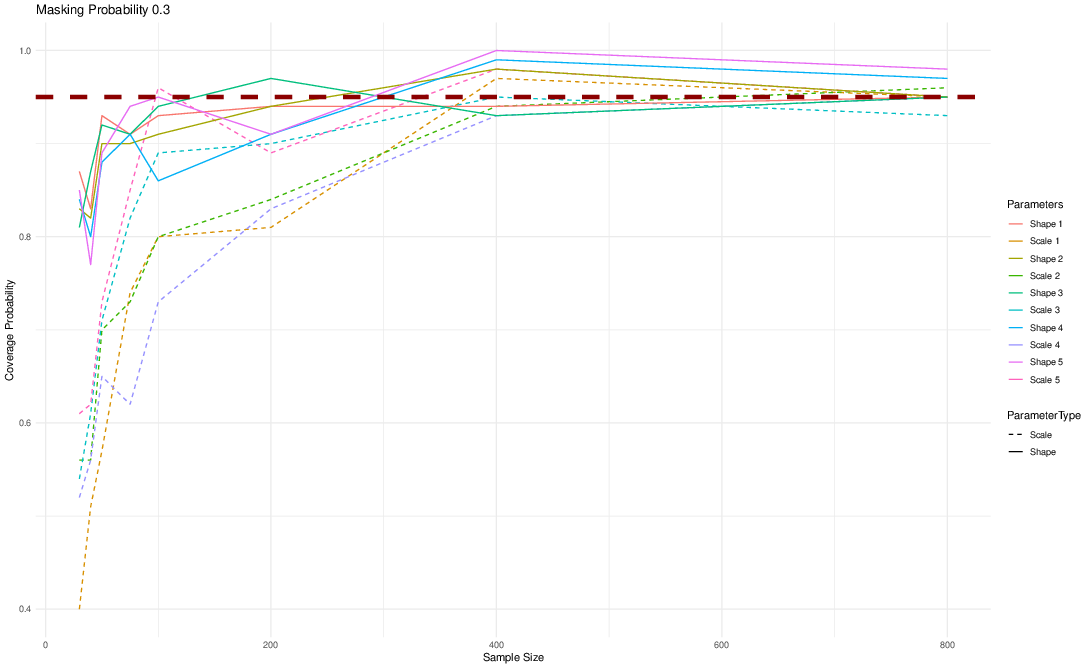
\includegraphics{image/plot-coverage-p_0.3-vs-sample-size} 

}

\caption{Coverage probability vs. sample size for masking probability $0.3$}\label{fig:plot-coverage-p-three-vs-sample-size}
\end{figure}

Here are some key observations:

\begin{enumerate}
\def\labelenumi{\arabic{enumi}.}
\item
  It is immediately obvious that the scale parameters (dashed lines)
  have a much lower coverage probability than the shape parameters
  (solid lines), particularly for small sample sizes less than
  \(n = 200\).

  In general, the scale parameters appear to be more difficult to
  estimate than the shape parameters.
\item
  As the sample size increases, the coverage probability for the shape
  parameters and scale parameters approaches the nominal level,
  \(95\%\).

  This suggests that the sampling distribution of the MLE is converging
  in distribution to a multivariate normal distribution with mean
  \(\boldsymbol{\theta}\) and variance-covariance given by the inverse
  of the FIM, consistent with the asymptotic theory.
\end{enumerate}

\hypertarget{scenario-coverage-probability-vs.-sample-size-and-masking-probability-without-right-censoring}{%
\paragraph*{Scenario: Coverage probability vs.~sample size and masking
probability without
right-censoring}\label{scenario-coverage-probability-vs.-sample-size-and-masking-probability-without-right-censoring}}
\addcontentsline{toc}{paragraph}{Scenario: Coverage probability
vs.~sample size and masking probability without right-censoring}

We want to get a larger picture of how the coverage probability depends
on the sample size \(n\) and masking probability \(p\). We fix the
right-censoring time to \(\tau = \infty\) and vary the sample size from
\(n = 30\) to \(n = 800\) and vary the masking probability from
\(p = 0\) (no masking) to \(p = 0.4\) and then compute the coverage
probability for each combination of sample size \(n\) and masking
probability \(p\).

\begin{figure}

{\centering 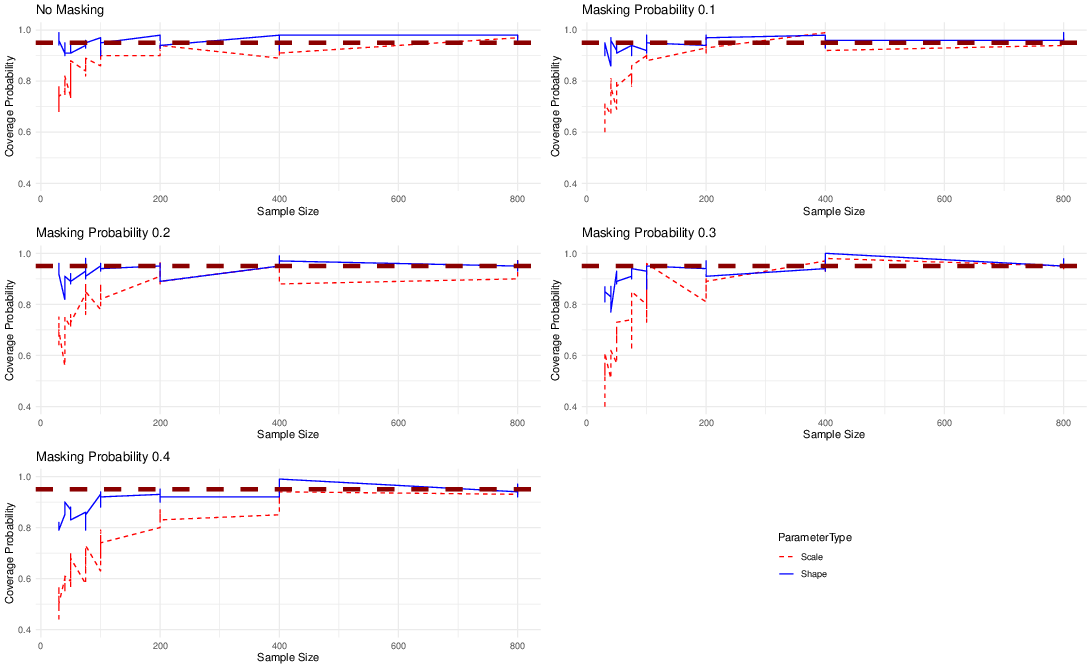
\includegraphics{image/plot-coverage-p-vs-sample-size} 

}

\caption{Coverage probability vs. sample size}\label{fig:plot-coverage-p-vs-sample-size}
\end{figure}

The results of this analysis are summarized by Figure
\ref{fig:plot-coverage-p-vs-sample-size}. Here are some key
observations:

\begin{enumerate}
\def\labelenumi{\arabic{enumi}.}
\item
  For sample sizes \(n \leq 100\), the coverage probability for the
  shape parameters is close to the nominal level, \(95\%\), only for
  small masking probabilities. However, as the sample size increases,
  the coverage probability for the shape parameters quickly approaches
  the nominal level, \(95\%\), for all masking probabilities reported
  here.
\item
  For the scale parameters, the coverage probability is too low for all
  sample sizes \(n < 200\) for all masking probabilities reported here.
  For small sample sizes, the confience intervals particularly for the
  scale parameters, should probably be taken with a grain of salt.
\end{enumerate}

In Section \ref{sec:boot}, we explore an alternative way to construct
confidence intervals using the bootstrap method, which is generally a
more accurate way to compute confidence intervals. Unlike the inverse of
the observed FIM, it does not assume that the sampling distribution of
the MLE is asymptotically normal, and so it is more robust to violations
of this assumption.

\hypertarget{confidence-interval-width}{%
\subsubsection{Confidence interval
width}\label{confidence-interval-width}}

We will use the inverse of the observed Fisher information matrix (FIM),
which was defined in Section \ref{sec:mle_properties}, to construct
\(95\%\)-confidence intervals for \(\boldsymbol{\theta}\) to compute the
confidence interval width of the MLE for each scenario. The confidence
interval width is defined as the difference between the upper and lower
bounds of the confidence interval.

If the confidence intervals are well-calibrated, a small confidence
interval width means we are more confident that the true value of
\(\boldsymbol{\theta}\) is close to the MLE, and a large confidence
interval width means we are less confident that the true value of
\(\boldsymbol{\theta}\) is close to the MLE. However, if the confidence
intervals are not well-calibrated, then the confidence interval width is
not particularly informative. See Section \ref{ec:coverage_prob} for a
discussion of well-calibrated confidence intervals, which we assume
here.

\begin{figure}

{\centering 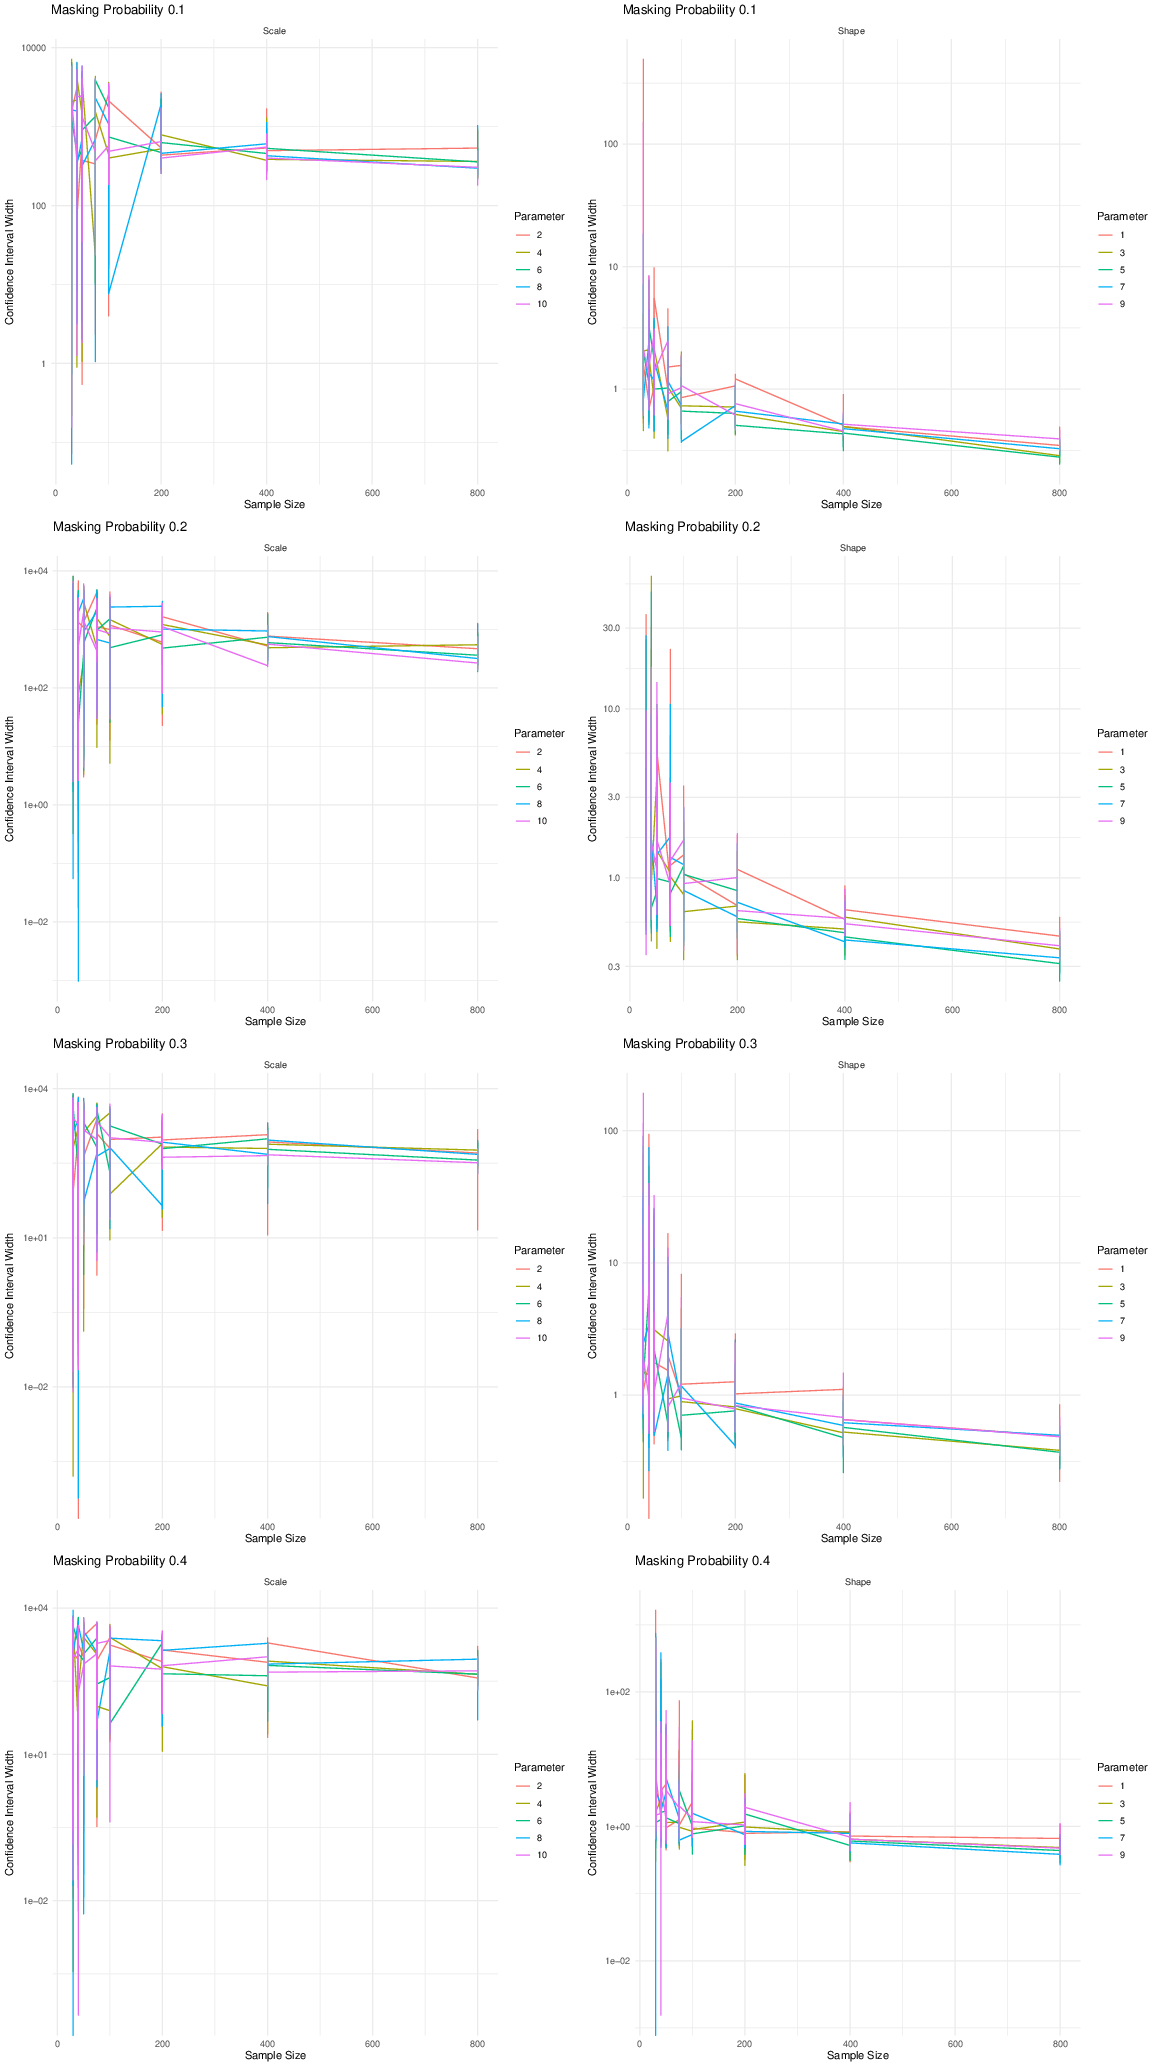
\includegraphics{image/ci-widths} 

}

\caption{Confidence interval widths vs. sample size}\label{fig:plot-ci-width-vs-sample-size}
\end{figure}

Some key observations:

\begin{enumerate}
\def\labelenumi{\arabic{enumi}.}
\item
  For the shape parameters, the confidence interval widths are small,
  but the true parameter values are also small. For the scale
  parameters, the confidence interval widths are large, but the true
  parameter values are also large.
\item
  For small sample sizes for every masking probability, the confidence
  interval widths are extremely variable, and since the coverage
  probability reported earlier showed they were not well-calibrated, we
  should not be confident in the MLE for small sample sizes. However,
  for large sample sizes, the confidence interval widths are relatively
  stable, and since the coverage probability reported earlier showed
  they were well-calibrated, we can be confident in the MLE for large
  sample sizes.
\item
  The confidence interval widths decrease at a decreasing rate as the
  sample size increases. This is expected since the inverse of the
  observed FIM scales as \(1/n\), and so the confidence interval widths
  should scale as \(1/\sqrt{n}\).

  On the one hand, this means that as the sample size increases, we see
  diminishing returns in the precision of the MLE, but on the other
  hand, the coverage probability is converging to the nominal level,
  \(95\%\), as the sample size increases, so we can at least gain
  confidence that the true parameter value is more likely to be within
  the reported confidence interval at the reported confidence level.
\item
  The confidence interval widths are somewhat sensitive to the masking
  probability. As the masking probability increases, the confidence
  interval widths increase.
\end{enumerate}

For the visualization code for the confidence widths, see Appendix C.

\hypertarget{variance}{%
\subsubsection{Variance}\label{variance}}

We estimate the precision of \(\boldsymbol{\hat\theta}\) with the
variance-covariance matrix, \[
\operatorname{Var}(\boldsymbol{\hat\theta}) =
    E\bigl(
        (\hat{\boldsymbol{\theta}} - E(\hat{\boldsymbol{\theta}}))
        (\hat{\boldsymbol{\theta}} - E(\hat{\boldsymbol{\theta}}))'
    \bigr),
\] which is a \(p\)-by-\(p\) matrix, where \(p\) is the number of
parameters, and again the the expectation is taken with respect to the
empirical sampling distribution. We will only report the diagonal
elements of the variance-covariance matrix, which are the variances of
the individual components of \(\boldsymbol{\hat\theta}\).

\begin{quote}
Dr.~Agustin: I didn't fill out variance and MSE sections. I have the
data, and most of the code for visualization. Would you like for me to
include any of these? I'm not sure about how large this paper should be.
\end{quote}

\hypertarget{mean-squared-error}{%
\subsubsection{Mean squared error}\label{mean-squared-error}}

The mean squared error, \(\operatorname{MSE}\), is a measure of
estimator error that incorporates both the bias and the variance, and is
defined as \[
\operatorname{MSE}(\boldsymbol{\hat\theta}) =
    E\bigl((\boldsymbol{\hat\theta} - \boldsymbol{\theta})(\boldsymbol{\hat\theta} - \boldsymbol{\theta})'\bigr) =
    \operatorname{Var}(\boldsymbol{\hat\theta}) +
    \operatorname{b}(\boldsymbol{\hat\theta})\operatorname{b}(\boldsymbol{\hat\theta})',
\] which is a \(p\)-by-\(p\) matrix, where \(p\) is the number of
parameters, and again the expectation is with respect to the empirical
sampling distribution. We will only report the diagoanl elements of the
MSE matrix, which are the mean squared errors of the individual
components of \(\boldsymbol{\hat\theta}\). Assuming the regularity
conditions for the MLE are met, the MSE converges in probability to the
variance, but for finite \(n\), the MSE is a more informative measure of
estimator error than the variance alone.

\hypertarget{sec:boot}{%
\subsection{Bootstrapping the sampling distribution of the
MLE}\label{sec:boot}}

In a real-world scenario, we would not know how to generate the data
from the underlying data generating process, and so we would not be able
to compute the empirical sampling distribution of the MLE.

However, we can use the bootstrap method. The bootstrap method is a
general method for estimating the sampling distribution of a statistic,
in our case the MLE. The most common form of the bootstrap is the
non-parametric bootstrap. In the non-parametric bootstrap, the random
data is created by resampling with replacement from the original data.
Since we do not know (nor attempt to model) the distribution of
candidate sets, this non-parametric form is ideal, since we can simply
resample from the original data to approximate its empirical sampling
distribution of the MLE.

We use the Weibull series data in {[}3{]} to illustrate the bootstrap
method. It's a real-world data set. We can estimate the sampling
distribution of the MLE using the bootstrap method, and compare these
results to the asymptotic theory. We expect that since the sample size
is relatively small, the bootstrap method will give us a better estimate
of the sampling distribution of the MLE than the asymptotic theory.

So, now we just resample from the data with replacement, and fit the
Weibull series model to each bootstrap sample. We do this \(B = 1000\)
times, giving us \(B\) bootstrap replicates of the MLE
\(\hat{\boldsymbol{\theta}}^{(1)},\ldots,\hat{\boldsymbol{\theta}}^{(B)}\).

We could then compute the bias, variance, MSE, and coverage probability
of the bootstrap replicates, and compare these results to the asymptotic
theory.

Earlier, we observed the inverse FIM provided for to small of a variance
of the component estimates for the MLE. So, we are going to use the
bootstrap method to provide better estimates.

We should see that the variance of the bootstrap replicates is larger
than the variance of the asymptotic theory, which should mitigate the
earlier problem of the inverse FIM providing too small of a variance of
the component estimates and thus resulting in poorly calibrated
confidence intervals.

This is particularly important for small sample sizes before the
asymptotic theory kicks in.

In Figure \ref{fig:ci-boot-shape}, we show the variance of the shape
paraemetes for the bootstrap replicates (blue) and the asymptotic theory
(green) for different sample sizes and differnet masking conditions. For
small sample sizes, the variance of the bootstrap replicates is larger
than the variance of the asymptotic theory, but they both converge to
the same value as the sample size increases.

\begin{figure}

{\centering 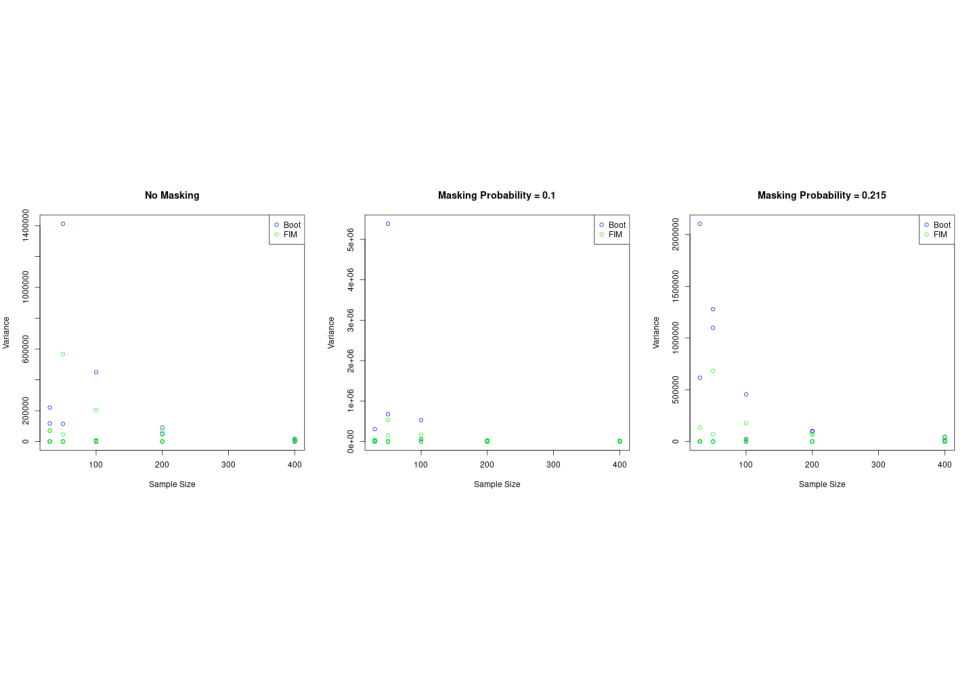
\includegraphics[width=1\linewidth]{wei_series_md_files/figure-latex/ci-boot-shape-1} 

}

\caption{Shape Parameters}\label{fig:ci-boot-shape}
\end{figure}

In Figure \ref{fig:ci-boot-scale}, we show the variance of the scale
parameters. Again, we see the same pattern emerge, where the variance of
the bootstrap replicates is larger than the variance of the asymptotic
theory for small sample sizes, but they both converge to the same value
as the sample size increases.

\begin{figure}

{\centering 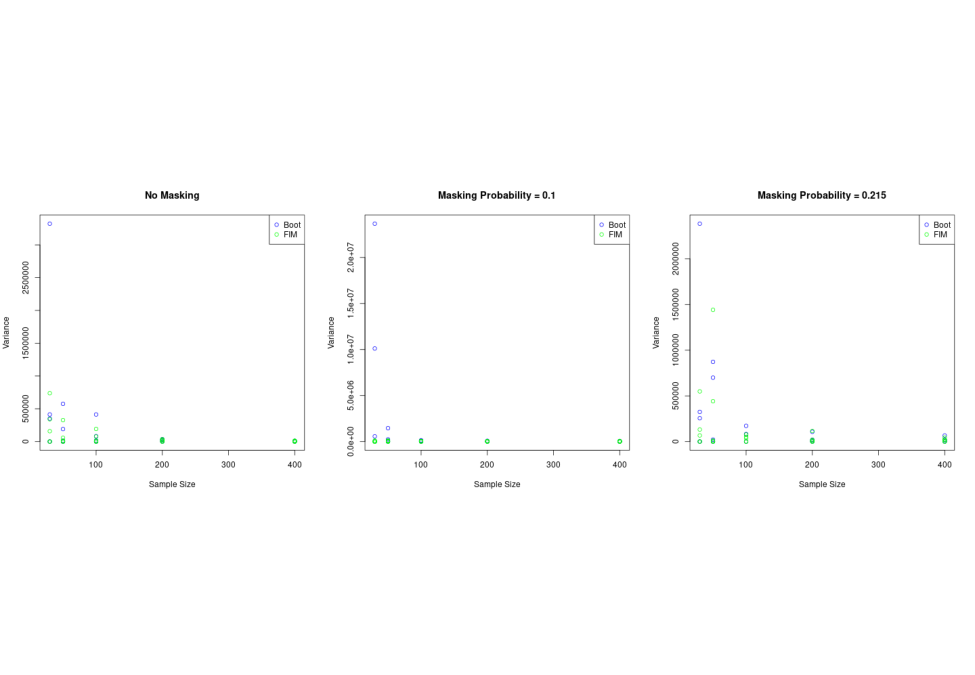
\includegraphics[width=1\linewidth]{wei_series_md_files/figure-latex/ci-boot-scale-1} 

}

\caption{Scale Parameters}\label{fig:ci-boot-scale}
\end{figure}

These corrections to the variance estimates should result in better
calibrated confidence intervals for small sample sizes.

\hypertarget{conclusion}{%
\section{Conclusion}\label{conclusion}}

We have developed a likelihood model for series systems with latent
components and right-censoring. We have provided evidence that, as long
as certain regularity conditions are met, the MLE is asymptotically
unbiased and consistent.

\hypertarget{references}{%
\section*{References}\label{references}}
\addcontentsline{toc}{section}{References}

Please see below for a full list of references.

\hypertarget{refs}{}
\begin{cslreferences}
\leavevmode\hypertarget{ref-Fran-1991}{}%
{[}1{]} \textsc{Guess}, F. M., \textsc{Hodgson}, T. J. and
\textsc{Usher}, J. S. (1991). Estimating system and component
reliabilities under partial information on cause of failure.
\emph{Journal of Statistical Planning and Inference} \textbf{29} 75--85.

\leavevmode\hypertarget{ref-bain}{}%
{[}2{]} \textsc{Engelhardt}, B. (1992). Introduction to probability and
mathematical statistics. 294.

\leavevmode\hypertarget{ref-Huairu-2013}{}%
{[}3{]} \textsc{Guo}, H., \textsc{Niu}, P. and \textsc{Szidarovszky}, F.
(2013). Estimating component reliabilities from incomplete system
failure data. \emph{Annual Reliability and Maintainability Symposium
(RAMS)} 1--6.
\end{cslreferences}

\hypertarget{appendix}{%
\section*{Appendix}\label{appendix}}
\addcontentsline{toc}{section}{Appendix}

\hypertarget{appendix-a-simulation-of-scenarios-using-the-monte-carlo-data-generating-process}{%
\subsection*{Appendix A: Simulation of scenarios using the Monte-carlo
data-generating
process}\label{appendix-a-simulation-of-scenarios-using-the-monte-carlo-data-generating-process}}
\addcontentsline{toc}{subsection}{Appendix A: Simulation of scenarios
using the Monte-carlo data-generating process}

\begin{Shaded}
\begin{Highlighting}[]
\CommentTok{\#\#\#\#\#\#\#\#\#\#\#\#\#\#\#\#\#\#\#\#\#\#\#\#\#\#\#\#\#\#\#\#\#\#\#\#\#\#\#\#\#\#\#\#\#\#\#\#\#\#\#\#\#\#\#\#\#\#\#\#\#}
\CommentTok{\# Simulation data generating process for specified scenario \#}
\CommentTok{\# (n, p, q), where:                                         \#}
\CommentTok{\#    {-} n is a vector of sample sizes                        \#}
\CommentTok{\#     {-} n is a vector of sample sizes                       \#}
\CommentTok{\#     {-} p is a vector of masking probabilities              \#}
\CommentTok{\#     {-} q is a vector of right{-}censoring quantiles of the   \#}
\CommentTok{\#       Weibull series distribution.}
\CommentTok{\#\#\#\#\#\#\#\#\#\#\#\#\#\#\#\#\#\#\#\#\#\#\#\#\#\#\#\#\#\#\#\#\#\#\#\#\#\#\#\#\#\#\#\#\#\#\#\#\#\#\#\#\#\#\#\#\#\#\#\#\#}

\CommentTok{\# here is the R libary we developed for this project}
\KeywordTok{library}\NormalTok{(wei.series.md.c1.c2.c3) }

\CommentTok{\# for parallel processing}
\KeywordTok{library}\NormalTok{(parallel)}

\CommentTok{\# you can set a seed for reproducibility of the experimental run}
\CommentTok{\# however, if you use parallel processing, this simple approach will not work.}
\KeywordTok{set.seed}\NormalTok{(}\DecValTok{1234}\NormalTok{)}

\CommentTok{\#\#\#\#\#\#\#\#\#\#\#\#\#\#\#\#\#\#\#\#\#\#\#\#\#\#\#\#\#\#\#\#\#\#\#\#\#\#\#\#\#\#\#\#\#\#\#}
\CommentTok{\# Here is an example of how to run a scenario \#}
\CommentTok{\#\#\#\#\#\#\#\#\#\#\#\#\#\#\#\#\#\#\#\#\#\#\#\#\#\#\#\#\#\#\#\#\#\#\#\#\#\#\#\#\#\#\#\#\#\#\#}

\CommentTok{\# set the simulation name to be used in the file names}
\NormalTok{sim.name \textless{}{-}}\StringTok{ "sim{-}2"}
\CommentTok{\# set the sample sizes}
\NormalTok{ns \textless{}{-}}\StringTok{ }\KeywordTok{c}\NormalTok{(}\DecValTok{30}\NormalTok{, }\DecValTok{40}\NormalTok{, }\DecValTok{50}\NormalTok{, }\DecValTok{75}\NormalTok{, }\DecValTok{100}\NormalTok{, }\DecValTok{200}\NormalTok{, }\DecValTok{400}\NormalTok{, }\DecValTok{800}\NormalTok{)}
\CommentTok{\# set the masking probabilities}
\NormalTok{ps \textless{}{-}}\StringTok{ }\KeywordTok{seq}\NormalTok{(}\DecValTok{0}\NormalTok{, }\DecValTok{0}\NormalTok{,}\DecValTok{1}\NormalTok{, }\FloatTok{0.2}\NormalTok{, }\FloatTok{0.3}\NormalTok{, }\FloatTok{0.4}\NormalTok{)}
\CommentTok{\# set the right{-}censoring quantiles}
\NormalTok{qs \textless{}{-}}\StringTok{ }\KeywordTok{c}\NormalTok{(}\FloatTok{0.5}\NormalTok{, }\FloatTok{0.6}\NormalTok{, }\FloatTok{0.7}\NormalTok{, }\FloatTok{0.8}\NormalTok{, }\FloatTok{0.9}\NormalTok{, }\FloatTok{0.95}\NormalTok{)}
\CommentTok{\# set the number of replicates}
\NormalTok{R \textless{}{-}}\StringTok{ }\DecValTok{100}
\CommentTok{\# set the number of CPU cores to use}
\NormalTok{ncores \textless{}{-}}\StringTok{ }\DecValTok{4}

\CommentTok{\# true parameter values}
\NormalTok{theta \textless{}{-}}\StringTok{ }\KeywordTok{c}\NormalTok{(}\DataTypeTok{shape1 =} \FloatTok{1.2576}\NormalTok{, }\DataTypeTok{scale1 =} \FloatTok{994.3661}\NormalTok{,}
           \DataTypeTok{shape2 =} \FloatTok{1.1635}\NormalTok{, }\DataTypeTok{scale2 =} \FloatTok{908.9458}\NormalTok{,}
           \DataTypeTok{shape3 =} \FloatTok{1.1308}\NormalTok{, }\DataTypeTok{scale3 =} \FloatTok{840.1141}\NormalTok{,}
           \DataTypeTok{shape4 =} \FloatTok{1.1802}\NormalTok{, }\DataTypeTok{scale4 =} \FloatTok{940.1141}\NormalTok{,}
           \DataTypeTok{shape5 =} \FloatTok{1.3311}\NormalTok{, }\DataTypeTok{scale5 =} \FloatTok{836.1123}\NormalTok{)}

\NormalTok{shapes \textless{}{-}}\StringTok{ }\NormalTok{theta[}\KeywordTok{seq}\NormalTok{(}\DecValTok{1}\NormalTok{, }\KeywordTok{length}\NormalTok{(theta), }\DecValTok{2}\NormalTok{)]}
\NormalTok{scales \textless{}{-}}\StringTok{ }\NormalTok{theta[}\KeywordTok{seq}\NormalTok{(}\DecValTok{2}\NormalTok{, }\KeywordTok{length}\NormalTok{(theta), }\DecValTok{2}\NormalTok{)]}

\CommentTok{\# helps the MLE optimization routine converge more quickly and reliably}
\CommentTok{\# by scaling the parameters to be of similar magnitude}
\NormalTok{parscale \textless{}{-}}\StringTok{ }\KeywordTok{c}\NormalTok{(}\DecValTok{1}\NormalTok{, }\DecValTok{1000}\NormalTok{, }\DecValTok{1}\NormalTok{, }\DecValTok{1000}\NormalTok{, }\DecValTok{1}\NormalTok{, }\DecValTok{1000}\NormalTok{, }\DecValTok{1}\NormalTok{, }\DecValTok{1000}\NormalTok{, }\DecValTok{1}\NormalTok{, }\DecValTok{1000}\NormalTok{)}

\NormalTok{sim.run \textless{}{-}}\StringTok{ }\ControlFlowTok{function}\NormalTok{(sim.name, n, p, q, }\DataTypeTok{R =} \DecValTok{1000}\NormalTok{) \{}
\NormalTok{    mles \textless{}{-}}\StringTok{ }\KeywordTok{list}\NormalTok{()}
\NormalTok{    problems \textless{}{-}}\StringTok{ }\KeywordTok{list}\NormalTok{()}

\NormalTok{    tau \textless{}{-}}\StringTok{ }\NormalTok{wei.series.md.c1.c2.c3}\OperatorTok{::}\KeywordTok{qwei\_series}\NormalTok{(}
        \DataTypeTok{p =}\NormalTok{ q, }\DataTypeTok{scales =}\NormalTok{ scales, }\DataTypeTok{shapes =}\NormalTok{ shapes)}

    \KeywordTok{cat}\NormalTok{(}\StringTok{"n ="}\NormalTok{, n, }\StringTok{", p ="}\NormalTok{, p, }\StringTok{", q = "}\NormalTok{, q, }\StringTok{", tau = "}\NormalTok{, tau, }\StringTok{"}\CharTok{\textbackslash{}n}\StringTok{"}\NormalTok{)}

    \ControlFlowTok{for}\NormalTok{ (r }\ControlFlowTok{in} \DecValTok{1}\OperatorTok{:}\NormalTok{R) \{}
\NormalTok{        result \textless{}{-}}\StringTok{ }\KeywordTok{tryCatch}\NormalTok{(\{}

\NormalTok{            df \textless{}{-}}\StringTok{ }\NormalTok{wei.series.md.c1.c2.c3}\OperatorTok{::}\KeywordTok{generate\_guo\_weibull\_table\_2\_data}\NormalTok{(}
                \DataTypeTok{shapes =}\NormalTok{ shapes,}
                \DataTypeTok{scales =}\NormalTok{ scales,}
                \DataTypeTok{n =}\NormalTok{ n,}
                \DataTypeTok{p =}\NormalTok{ p,}
                \DataTypeTok{tau =}\NormalTok{ tau)}

\NormalTok{            sol \textless{}{-}}\StringTok{ }\NormalTok{wei.series.md.c1.c2.c3}\OperatorTok{::}\KeywordTok{mle\_nelder\_wei\_series\_md\_c1\_c2\_c3}\NormalTok{(}
                \DataTypeTok{df =}\NormalTok{ df,}
                \DataTypeTok{theta0 =}\NormalTok{ theta,}
                \DataTypeTok{reltol =} \FloatTok{1e{-}7}\NormalTok{,}
                \DataTypeTok{parscale =}\NormalTok{ parscale,}
                \DataTypeTok{maxit =}\NormalTok{ 2000L)}
\NormalTok{            mles \textless{}{-}}\StringTok{ }\KeywordTok{append}\NormalTok{(mles, }\KeywordTok{list}\NormalTok{(sol))}

            \ControlFlowTok{if}\NormalTok{ (r }\OperatorTok{\%\%}\StringTok{ }\DecValTok{10} \OperatorTok{==}\StringTok{ }\DecValTok{0}\NormalTok{) \{}
                \KeywordTok{cat}\NormalTok{(}\StringTok{"r = "}\NormalTok{, r, }\StringTok{": "}\NormalTok{, sol}\OperatorTok{$}\NormalTok{par, }\StringTok{"}\CharTok{\textbackslash{}n}\StringTok{"}\NormalTok{)}
\NormalTok{            \}}

\NormalTok{        \}, }\DataTypeTok{error =} \ControlFlowTok{function}\NormalTok{(e) \{}
            \KeywordTok{cat}\NormalTok{(}\StringTok{"Error at iteration"}\NormalTok{, r, }\StringTok{":"}\NormalTok{)}
            \KeywordTok{print}\NormalTok{(e)}
\NormalTok{            problems \textless{}{-}}\StringTok{ }\KeywordTok{append}\NormalTok{(problems, }\KeywordTok{list}\NormalTok{(}\KeywordTok{list}\NormalTok{(}
                \DataTypeTok{error =}\NormalTok{ e, }\DataTypeTok{n =}\NormalTok{ n, }\DataTypeTok{p =}\NormalTok{ p, }\DataTypeTok{q =}\NormalTok{ q, }\DataTypeTok{tau =}\NormalTok{ tau, }\DataTypeTok{df =}\NormalTok{ df)))}
\NormalTok{        \})}
\NormalTok{    \}}
  
    \ControlFlowTok{if}\NormalTok{ (}\KeywordTok{length}\NormalTok{(mles) }\OperatorTok{!=}\StringTok{ }\DecValTok{0}\NormalTok{) \{}
        \KeywordTok{saveRDS}\NormalTok{(}\KeywordTok{list}\NormalTok{(}\DataTypeTok{n =}\NormalTok{ n, }\DataTypeTok{p =}\NormalTok{ p, }\DataTypeTok{q =}\NormalTok{ q, }\DataTypeTok{tau =}\NormalTok{ tau, }\DataTypeTok{mles =}\NormalTok{ mles),}
            \DataTypeTok{file =} \KeywordTok{paste0}\NormalTok{(}\StringTok{"./results/"}\NormalTok{, sim.name, }\StringTok{"/results\_"}\NormalTok{, n, }\StringTok{"\_"}\NormalTok{, p, }\StringTok{"\_"}\NormalTok{, q, }\StringTok{".rds"}\NormalTok{))}
\NormalTok{    \}}

    \ControlFlowTok{if}\NormalTok{ (}\KeywordTok{length}\NormalTok{(problems) }\OperatorTok{!=}\StringTok{ }\DecValTok{0}\NormalTok{) \{}
        \KeywordTok{saveRDS}\NormalTok{(}\KeywordTok{list}\NormalTok{(}\DataTypeTok{n =}\NormalTok{ n, }\DataTypeTok{p =}\NormalTok{ p, }\DataTypeTok{q =}\NormalTok{ q, }\DataTypeTok{tau =}\NormalTok{ tau, }\DataTypeTok{problems =}\NormalTok{ problems),}
            \DataTypeTok{file =} \KeywordTok{paste0}\NormalTok{(}\StringTok{"./problems/"}\NormalTok{, sim.name, }\StringTok{"/problems\_"}\NormalTok{, n, }\StringTok{"\_"}\NormalTok{, p, }\StringTok{"\_"}\NormalTok{, q, }\StringTok{".rds"}\NormalTok{))}
\NormalTok{    \}}
\NormalTok{\}}

\NormalTok{params \textless{}{-}}\StringTok{ }\KeywordTok{expand.grid}\NormalTok{(}\DataTypeTok{n =}\NormalTok{ ns, }\DataTypeTok{p =}\NormalTok{ ps, }\DataTypeTok{q =}\NormalTok{ qs)}
\NormalTok{result \textless{}{-}}\StringTok{ }\KeywordTok{mclapply}\NormalTok{(}
    \DecValTok{1}\OperatorTok{:}\KeywordTok{nrow}\NormalTok{(params),}
    \ControlFlowTok{function}\NormalTok{(i) }\KeywordTok{sim.run}\NormalTok{(sim.name, params}\OperatorTok{$}\NormalTok{n[i], params}\OperatorTok{$}\NormalTok{p[i], params}\OperatorTok{$}\NormalTok{q[i], R),}
    \DataTypeTok{mc.cores =}\NormalTok{ ncores)}
\end{Highlighting}
\end{Shaded}

\hypertarget{appendix-b-simulation-of-scenarios-using-the-bootstrap-method}{%
\subsection*{Appendix B: Simulation of scenarios using the Bootstrap
method}\label{appendix-b-simulation-of-scenarios-using-the-bootstrap-method}}
\addcontentsline{toc}{subsection}{Appendix B: Simulation of scenarios
using the Bootstrap method}

\begin{Shaded}
\begin{Highlighting}[]
\CommentTok{\#\#\#\#\#\#\#\#\#\#\#\#\#\#\#\#\#\#\#\#\#\#\#\#\#\#\#\#\#\#\#\#\#\#\#\#\#\#\#\#\#\#\#\#\#\#\#\#\#\#\#\#\#\#\#\#\#\#\#\#\#}
\CommentTok{\# in this scenario, we want to see how we can use the bootstrap}
\CommentTok{\# method to estimate the confidence intervals more precisely (better calibration}
\CommentTok{\# of confidence intervals) for small sample sizes.}
\CommentTok{\# we\textquotesingle{}ll use it to construct a 95\% confidence interval for the estimator. we\textquotesingle{}ll}
\CommentTok{\# compare this result to the asymptotic theory confidence interval.}
\CommentTok{\# finally, we\textquotesingle{}ll generate CIs by each method, asymptotic (inverse FIM) and }
\CommentTok{\# bootstrap (cov), and compare the coverage probabilities.}
\CommentTok{\#\#\#\#\#\#\#\#\#\#\#\#\#\#\#\#\#\#\#\#\#\#\#\#\#\#\#\#\#\#\#\#\#\#\#\#\#\#\#\#\#\#\#\#\#\#\#\#\#\#\#\#\#\#\#\#\#\#\#\#\#}

\KeywordTok{library}\NormalTok{(boot)}
\KeywordTok{library}\NormalTok{(parallel)}
\KeywordTok{library}\NormalTok{(wei.series.md.c1.c2.c3)}

\NormalTok{theta \textless{}{-}}\StringTok{ }\KeywordTok{c}\NormalTok{(}\DataTypeTok{shape1 =} \FloatTok{1.2576}\NormalTok{, }\DataTypeTok{scale1 =} \FloatTok{994.3661}\NormalTok{,}
           \DataTypeTok{shape2 =} \FloatTok{1.1635}\NormalTok{, }\DataTypeTok{scale2 =} \FloatTok{908.9458}\NormalTok{,}
           \DataTypeTok{shape3 =} \FloatTok{1.1308}\NormalTok{, }\DataTypeTok{scale3 =} \FloatTok{840.1141}\NormalTok{,}
           \DataTypeTok{shape4 =} \FloatTok{1.1802}\NormalTok{, }\DataTypeTok{scale4 =} \FloatTok{940.1141}\NormalTok{,}
           \DataTypeTok{shape5 =} \FloatTok{1.3311}\NormalTok{, }\DataTypeTok{scale5 =} \FloatTok{836.1123}\NormalTok{)}

\NormalTok{shapes \textless{}{-}}\StringTok{ }\NormalTok{theta[}\KeywordTok{seq}\NormalTok{(}\DecValTok{1}\NormalTok{, }\KeywordTok{length}\NormalTok{(theta), }\DecValTok{2}\NormalTok{)]}
\NormalTok{scales \textless{}{-}}\StringTok{ }\NormalTok{theta[}\KeywordTok{seq}\NormalTok{(}\DecValTok{2}\NormalTok{, }\KeywordTok{length}\NormalTok{(theta), }\DecValTok{2}\NormalTok{)]}

\CommentTok{\# number of CPU cores to use in bootstrap for parallel processing}
\NormalTok{ncores \textless{}{-}}\StringTok{ }\DecValTok{4}

\CommentTok{\# helps the MLE optimization routine converge more quickly and reliably}
\NormalTok{parscale \textless{}{-}}\StringTok{ }\KeywordTok{c}\NormalTok{(}\DecValTok{1}\NormalTok{, }\DecValTok{1000}\NormalTok{, }\DecValTok{1}\NormalTok{, }\DecValTok{1000}\NormalTok{, }\DecValTok{1}\NormalTok{, }\DecValTok{1000}\NormalTok{, }\DecValTok{1}\NormalTok{, }\DecValTok{1000}\NormalTok{, }\DecValTok{1}\NormalTok{, }\DecValTok{1000}\NormalTok{)}

\CommentTok{\#set.seed(134849131)}

\CommentTok{\# sample sizes}
\NormalTok{ns \textless{}{-}}\StringTok{ }\KeywordTok{c}\NormalTok{(}\DecValTok{30}\NormalTok{, }\DecValTok{50}\NormalTok{, }\DecValTok{100}\NormalTok{, }\DecValTok{200}\NormalTok{, }\DecValTok{400}\NormalTok{)}
\CommentTok{\# masking probabilities, no masking and 21.5\% masking}
\NormalTok{ps \textless{}{-}}\StringTok{ }\KeywordTok{c}\NormalTok{(}\DecValTok{0}\NormalTok{, }\FloatTok{0.215}\NormalTok{)}
\CommentTok{\# quantiles of weibull series distribution, no right{-}censoring and 25\% right{-}censoring}
\NormalTok{qs \textless{}{-}}\StringTok{ }\KeywordTok{c}\NormalTok{(}\DecValTok{1}\NormalTok{, }\FloatTok{0.75}\NormalTok{)}

\NormalTok{sim.name \textless{}{-}}\StringTok{ "sim{-}1{-}boot"}

\NormalTok{sim.boot.run \textless{}{-}}\StringTok{ }\ControlFlowTok{function}\NormalTok{(n, p, q, }\DataTypeTok{R =} \DecValTok{1000}\NormalTok{) \{}

\NormalTok{    problems \textless{}{-}}\StringTok{ }\KeywordTok{list}\NormalTok{()}

\NormalTok{    tau \textless{}{-}}\StringTok{ }\NormalTok{wei.series.md.c1.c2.c3}\OperatorTok{::}\KeywordTok{qwei\_series}\NormalTok{(}
        \DataTypeTok{p =}\NormalTok{ q, }\DataTypeTok{scales =}\NormalTok{ scales, }\DataTypeTok{shapes =}\NormalTok{ shapes)}

    \KeywordTok{cat}\NormalTok{(}\StringTok{"n ="}\NormalTok{, n, }\StringTok{", p ="}\NormalTok{, p, }\StringTok{", q = "}\NormalTok{, q, }\StringTok{", tau = "}\NormalTok{, tau, }\StringTok{"}\CharTok{\textbackslash{}n}\StringTok{"}\NormalTok{)}
  
\NormalTok{    result \textless{}{-}}\StringTok{ }\KeywordTok{tryCatch}\NormalTok{(\{}
\NormalTok{        df \textless{}{-}}\StringTok{ }\NormalTok{wei.series.md.c1.c2.c3}\OperatorTok{::}\KeywordTok{generate\_guo\_weibull\_table\_2\_data}\NormalTok{(}
            \DataTypeTok{shapes =}\NormalTok{ shapes,}
            \DataTypeTok{scales =}\NormalTok{ scales,}
            \DataTypeTok{n =}\NormalTok{ n,}
            \DataTypeTok{p =}\NormalTok{ p,}
            \DataTypeTok{tau =}\NormalTok{ tau)}

\NormalTok{        sol \textless{}{-}}\StringTok{ }\NormalTok{wei.series.md.c1.c2.c3}\OperatorTok{::}\KeywordTok{mle\_nelder\_wei\_series\_md\_c1\_c2\_c3}\NormalTok{(}
            \DataTypeTok{df =}\NormalTok{ df,}
            \DataTypeTok{theta0 =}\NormalTok{ theta,}
            \DataTypeTok{reltol =} \FloatTok{1e{-}7}\NormalTok{,}
            \DataTypeTok{parscale =}\NormalTok{ parscale,}
            \DataTypeTok{maxit =}\NormalTok{ 2000L)}

        \KeywordTok{cat}\NormalTok{(}\StringTok{"mle: "}\NormalTok{, sol}\OperatorTok{$}\NormalTok{par, }\StringTok{"}\CharTok{\textbackslash{}n}\StringTok{"}\NormalTok{)}

\NormalTok{        sol.boot \textless{}{-}}\StringTok{ }\KeywordTok{boot}\NormalTok{(df, }\ControlFlowTok{function}\NormalTok{(df, i) \{}
\NormalTok{            sol \textless{}{-}}\StringTok{ }\NormalTok{wei.series.md.c1.c2.c3}\OperatorTok{::}\KeywordTok{mle\_nelder\_wei\_series\_md\_c1\_c2\_c3}\NormalTok{(}
                \DataTypeTok{df =}\NormalTok{ df[i, ],}
                \DataTypeTok{theta0 =}\NormalTok{ sol}\OperatorTok{$}\NormalTok{par,}
                \DataTypeTok{reltol =} \FloatTok{1e{-}7}\NormalTok{,}
                \DataTypeTok{parscale =}\NormalTok{ parscale,}
                \DataTypeTok{maxit =}\NormalTok{ 1000L)}
            \KeywordTok{cat}\NormalTok{(}\StringTok{"boot: "}\NormalTok{, sol}\OperatorTok{$}\NormalTok{par, }\StringTok{"}\CharTok{\textbackslash{}n}\StringTok{"}\NormalTok{)}
\NormalTok{            sol}\OperatorTok{$}\NormalTok{par}
\NormalTok{        \}, }\DataTypeTok{ncpus =}\NormalTok{ ncores, }\DataTypeTok{R =}\NormalTok{ R)}

        \KeywordTok{saveRDS}\NormalTok{(}\KeywordTok{list}\NormalTok{(}\DataTypeTok{n =}\NormalTok{ n, }\DataTypeTok{p =}\NormalTok{ p, }\DataTypeTok{q =}\NormalTok{ q, }\DataTypeTok{tau =}\NormalTok{ tau, }\DataTypeTok{mle =}\NormalTok{ sol, }\DataTypeTok{mle.boot =}\NormalTok{ sol.boot),}
            \DataTypeTok{file =} \KeywordTok{paste0}\NormalTok{(}\StringTok{"./results/"}\NormalTok{, sim.name, }\StringTok{"/results\_"}\NormalTok{, n, }\StringTok{"\_"}\NormalTok{, p, }\StringTok{"\_"}\NormalTok{, q, }\StringTok{".rds"}\NormalTok{))}

\NormalTok{        \}, }\DataTypeTok{error =} \ControlFlowTok{function}\NormalTok{(e) \{}
            \KeywordTok{print}\NormalTok{(e)}
\NormalTok{            problems \textless{}{-}}\StringTok{ }\KeywordTok{append}\NormalTok{(problems, }\KeywordTok{list}\NormalTok{(}\KeywordTok{list}\NormalTok{(}
                \DataTypeTok{error =}\NormalTok{ e, }\DataTypeTok{n =}\NormalTok{ n, }\DataTypeTok{p =}\NormalTok{ p, }\DataTypeTok{q =}\NormalTok{ q, }\DataTypeTok{tau =}\NormalTok{ tau, }\DataTypeTok{df =}\NormalTok{ df)))}
\NormalTok{        \})}

    \ControlFlowTok{if}\NormalTok{ (}\KeywordTok{length}\NormalTok{(problems) }\OperatorTok{!=}\StringTok{ }\DecValTok{0}\NormalTok{) \{}
        \KeywordTok{saveRDS}\NormalTok{(}\KeywordTok{list}\NormalTok{(}\DataTypeTok{n =}\NormalTok{ n, }\DataTypeTok{p =}\NormalTok{ p, }\DataTypeTok{q =}\NormalTok{ q, }\DataTypeTok{tau =}\NormalTok{ tau, }\DataTypeTok{problems =}\NormalTok{ problems),}
                \DataTypeTok{file =} \KeywordTok{paste0}\NormalTok{(}\StringTok{"./problems/"}\NormalTok{, sim.name, }\StringTok{"/problems\_"}\NormalTok{, n, }\StringTok{"\_"}\NormalTok{, p, }\StringTok{"\_"}\NormalTok{, q, }\StringTok{".rds"}\NormalTok{))}
\NormalTok{    \}}
\NormalTok{\}}
  
\NormalTok{params \textless{}{-}}\StringTok{ }\KeywordTok{expand.grid}\NormalTok{(}\DataTypeTok{n =}\NormalTok{ ns, }\DataTypeTok{p =}\NormalTok{ ps, }\DataTypeTok{q =}\NormalTok{ qs)}
\NormalTok{result \textless{}{-}}\StringTok{ }\KeywordTok{mclapply}\NormalTok{(}
    \DecValTok{1}\OperatorTok{:}\KeywordTok{nrow}\NormalTok{(params),}
    \ControlFlowTok{function}\NormalTok{(i) }\KeywordTok{sim.boot.run}\NormalTok{(sim.name, params}\OperatorTok{$}\NormalTok{n[i], params}\OperatorTok{$}\NormalTok{p[i], params}\OperatorTok{$}\NormalTok{q[i]),}
    \DataTypeTok{mc.cores =}\NormalTok{ ncores)}
\end{Highlighting}
\end{Shaded}

\hypertarget{appendix-c-confidence-width-visualizations}{%
\subsection*{Appendix C: Confidence width
visualizations}\label{appendix-c-confidence-width-visualizations}}
\addcontentsline{toc}{subsection}{Appendix C: Confidence width
visualizations}

\begin{Shaded}
\begin{Highlighting}[]
\CommentTok{\#\#\#\#\#\#\#\#\#\#\#\#\#\#\#\#\#\#\#\#\#\#\#\#\#\#\#\#\#\#\#\#\#\#\#\#\#\#\#\#\#\#\#\#\#\#\#\#\#\#\#\#\#\#\#\#\#\#\#\#\#\#\#\#\#\#\#}
\CommentTok{\# we visualize CI width as a function of                          \#}
\CommentTok{\# masking component cause of failure p from p = 0 to p = 0.4      \#}
\CommentTok{\# and sample size n. we have R = 100 replicates for each p and n. \#}
\CommentTok{\#\#\#\#\#\#\#\#\#\#\#\#\#\#\#\#\#\#\#\#\#\#\#\#\#\#\#\#\#\#\#\#\#\#\#\#\#\#\#\#\#\#\#\#\#\#\#\#\#\#\#\#\#\#\#\#\#\#\#\#\#\#\#\#\#\#\#}
\KeywordTok{library}\NormalTok{(gridExtra)  }\CommentTok{\# for arranging plots}
\KeywordTok{library}\NormalTok{(ggplot2)}
\KeywordTok{library}\NormalTok{(tidyverse)}
\KeywordTok{library}\NormalTok{(dplyr)}
\KeywordTok{library}\NormalTok{(algebraic.mle)}
\KeywordTok{library}\NormalTok{(md.tools)}
\KeywordTok{library}\NormalTok{(wei.series.md.c1.c2.c3)}

\NormalTok{theta \textless{}{-}}\StringTok{ }\KeywordTok{c}\NormalTok{(}\DataTypeTok{shape1 =} \FloatTok{1.2576}\NormalTok{, }\DataTypeTok{scale1 =} \FloatTok{994.3661}\NormalTok{,}
           \DataTypeTok{shape2 =} \FloatTok{1.1635}\NormalTok{, }\DataTypeTok{scale2 =} \FloatTok{908.9458}\NormalTok{,}
           \DataTypeTok{shape3 =} \FloatTok{1.1308}\NormalTok{, }\DataTypeTok{scale3 =} \FloatTok{840.1141}\NormalTok{,}
           \DataTypeTok{shape4 =} \FloatTok{1.1802}\NormalTok{, }\DataTypeTok{scale4 =} \FloatTok{940.1141}\NormalTok{,}
           \DataTypeTok{shape5 =} \FloatTok{1.3311}\NormalTok{, }\DataTypeTok{scale5 =} \FloatTok{836.1123}\NormalTok{)}

\NormalTok{shapes \textless{}{-}}\StringTok{ }\NormalTok{theta[}\KeywordTok{seq}\NormalTok{(}\DecValTok{1}\NormalTok{, }\KeywordTok{length}\NormalTok{(theta), }\DecValTok{2}\NormalTok{)]}
\NormalTok{scales \textless{}{-}}\StringTok{ }\NormalTok{theta[}\KeywordTok{seq}\NormalTok{(}\DecValTok{2}\NormalTok{, }\KeywordTok{length}\NormalTok{(theta), }\DecValTok{2}\NormalTok{)]}
\NormalTok{sim2\_n \textless{}{-}}\StringTok{ }\KeywordTok{c}\NormalTok{(}\DecValTok{30}\NormalTok{, }\DecValTok{40}\NormalTok{, }\DecValTok{50}\NormalTok{, }\DecValTok{75}\NormalTok{, }\DecValTok{100}\NormalTok{, }\DecValTok{200}\NormalTok{, }\DecValTok{400}\NormalTok{, }\DecValTok{800}\NormalTok{)}

\CommentTok{\#\#\#\#\#\#\#\#\#\#\#\#\#\#\#\#\#\#\#\#\#\#\#\#\#\#\#\#\#\#}
\CommentTok{\# generate CI width function \#}
\CommentTok{\#\#\#\#\#\#\#\#\#\#\#\#\#\#\#\#\#\#\#\#\#\#\#\#\#\#\#\#\#\#}
\NormalTok{gen\_ci\_width \textless{}{-}}\StringTok{ }\ControlFlowTok{function}\NormalTok{(sim\_p\_mles, sim\_p) \{}

\NormalTok{    ci\_widths \textless{}{-}}\StringTok{ }\KeywordTok{list}\NormalTok{()}

    \ControlFlowTok{for}\NormalTok{ (i }\ControlFlowTok{in} \DecValTok{1}\OperatorTok{:}\KeywordTok{length}\NormalTok{(sim\_p)) \{}

\NormalTok{        ci\_widths[[i]] \textless{}{-}}\StringTok{ }\KeywordTok{matrix}\NormalTok{(}\DataTypeTok{nrow =} \KeywordTok{length}\NormalTok{(sim\_p\_mles[[i]]), }\DataTypeTok{ncol =} \KeywordTok{length}\NormalTok{(theta))}

        \ControlFlowTok{for}\NormalTok{ (j }\ControlFlowTok{in} \DecValTok{1}\OperatorTok{:}\KeywordTok{length}\NormalTok{(sim\_p\_mles[[i]])) \{}
\NormalTok{            theta.hat \textless{}{-}}\StringTok{ }\NormalTok{algebraic.mle}\OperatorTok{::}\KeywordTok{mle\_numerical}\NormalTok{(sim\_p\_mles[[i]][[j]])}
            \CommentTok{\# this is a m x 2 matrix, where m is the number of parameters}
\NormalTok{            ci \textless{}{-}}\StringTok{ }\KeywordTok{confint}\NormalTok{(theta.hat, }\DataTypeTok{use\_t\_dist =} \OtherTok{FALSE}\NormalTok{)}

            \ControlFlowTok{if}\NormalTok{ (}\KeywordTok{any}\NormalTok{(}\KeywordTok{is.na}\NormalTok{(ci))) \{}
                \ControlFlowTok{next}
\NormalTok{            \}}

\NormalTok{            ci\_widths[[i]][j,] \textless{}{-}}\StringTok{ }\NormalTok{ci[,}\DecValTok{2}\NormalTok{] }\OperatorTok{{-}}\StringTok{ }\NormalTok{ci[,}\DecValTok{1}\NormalTok{]}
\NormalTok{        \}}
\NormalTok{    \}}

\NormalTok{    ci\_widths}
\NormalTok{\}}

\CommentTok{\#\#\#\#\#\#\#\#\#\#\#\#\#\#\#\#\#\#\#\#\#\#\#\#\#\#\#\#\#\#\#\#\#\#\#}
\CommentTok{\# generate CI width plot function \#}
\CommentTok{\#\#\#\#\#\#\#\#\#\#\#\#\#\#\#\#\#\#\#\#\#\#\#\#\#\#\#\#\#\#\#\#\#\#\#}
\NormalTok{gen\_ci\_width\_plot \textless{}{-}}\StringTok{ }\ControlFlowTok{function}\NormalTok{(ci\_widths, sim\_n, p) \{}

\NormalTok{    ci\_widths\_df \textless{}{-}}\StringTok{ }\KeywordTok{do.call}\NormalTok{(rbind, }\KeywordTok{lapply}\NormalTok{(}\KeywordTok{seq\_along}\NormalTok{(ci\_widths), }\ControlFlowTok{function}\NormalTok{(i) \{}
    \KeywordTok{data.frame}\NormalTok{(}\DataTypeTok{SampleSize =} \KeywordTok{rep}\NormalTok{(sim\_n[i], }\KeywordTok{nrow}\NormalTok{(ci\_widths[[i]])),}
                \DataTypeTok{CI\_Width =} \KeywordTok{as.vector}\NormalTok{(ci\_widths[[i]]),}
                \DataTypeTok{Parameter =} \KeywordTok{rep}\NormalTok{(}\KeywordTok{seq}\NormalTok{(}\KeywordTok{ncol}\NormalTok{(ci\_widths[[i]])), }\DataTypeTok{each =} \KeywordTok{nrow}\NormalTok{(ci\_widths[[i]])),}
                \DataTypeTok{Type =} \KeywordTok{rep}\NormalTok{(}\KeywordTok{c}\NormalTok{(}\StringTok{"Shape"}\NormalTok{, }\StringTok{"Scale"}\NormalTok{), }\DataTypeTok{each =} \KeywordTok{nrow}\NormalTok{(ci\_widths[[i]]), }\DataTypeTok{times =} \KeywordTok{ncol}\NormalTok{(ci\_widths[[i]]) }\OperatorTok{/}\StringTok{ }\DecValTok{2}\NormalTok{))}
\NormalTok{    \}))}

    \CommentTok{\# Split the data frame based on parameter type (Scale or Shape)}
\NormalTok{    ci\_widths\_list \textless{}{-}}\StringTok{ }\KeywordTok{split}\NormalTok{(ci\_widths\_df, ci\_widths\_df}\OperatorTok{$}\NormalTok{Type)}
    \CommentTok{\# Generate a plot for each type, using a log y scale}
\NormalTok{    plots \textless{}{-}}\StringTok{ }\KeywordTok{lapply}\NormalTok{(ci\_widths\_list, }\ControlFlowTok{function}\NormalTok{(df) \{}
        \KeywordTok{ggplot}\NormalTok{(df, }\KeywordTok{aes}\NormalTok{(}\DataTypeTok{x =}\NormalTok{ SampleSize, }\DataTypeTok{y =}\NormalTok{ CI\_Width, }\DataTypeTok{color =} \KeywordTok{factor}\NormalTok{(Parameter))) }\OperatorTok{+}
\StringTok{            }\KeywordTok{geom\_line}\NormalTok{() }\OperatorTok{+}\StringTok{ }
\StringTok{            }\KeywordTok{scale\_y\_log10}\NormalTok{() }\OperatorTok{+}
\StringTok{            }\KeywordTok{labs}\NormalTok{(}\DataTypeTok{title =} \KeywordTok{paste}\NormalTok{(}\StringTok{"Masking Probability"}\NormalTok{, p),}
                \DataTypeTok{x =} \StringTok{"Sample Size"}\NormalTok{, }\DataTypeTok{y =} \StringTok{"Confidence Interval Width"}\NormalTok{, }\DataTypeTok{color =} \StringTok{"Parameter"}\NormalTok{) }\OperatorTok{+}
\StringTok{            }\KeywordTok{facet\_wrap}\NormalTok{(}\OperatorTok{\textasciitilde{}}\StringTok{ }\NormalTok{Type, }\DataTypeTok{scales =} \StringTok{"free"}\NormalTok{) }\OperatorTok{+}
\StringTok{            }\KeywordTok{theme\_minimal}\NormalTok{()}
\NormalTok{    \})}

    \CommentTok{\# Arrange the plots in a grid}
    \KeywordTok{grid.arrange}\NormalTok{(}\DataTypeTok{grobs =}\NormalTok{ plots, }\DataTypeTok{ncol =} \DecValTok{2}\NormalTok{)}
\NormalTok{\}}

\CommentTok{\#\#\#\#\#\#\#\#\#\#\#}
\CommentTok{\# p = 0.1 \#}
\CommentTok{\#\#\#\#\#\#\#\#\#\#\#}
\NormalTok{sim2\_}\DecValTok{30}\NormalTok{\_}\FloatTok{0.1}\NormalTok{ \textless{}{-}}\StringTok{ }\KeywordTok{readRDS}\NormalTok{(}\StringTok{"results/sim{-}2/results\_30\_0.1\_1.rds"}\NormalTok{)}
\NormalTok{sim2\_}\DecValTok{40}\NormalTok{\_}\FloatTok{0.1}\NormalTok{ \textless{}{-}}\StringTok{ }\KeywordTok{readRDS}\NormalTok{(}\StringTok{"results/sim{-}2/results\_40\_0.1\_1.rds"}\NormalTok{)}
\NormalTok{sim2\_}\DecValTok{50}\NormalTok{\_}\FloatTok{0.1}\NormalTok{ \textless{}{-}}\StringTok{ }\KeywordTok{readRDS}\NormalTok{(}\StringTok{"results/sim{-}2/results\_50\_0.1\_1.rds"}\NormalTok{)}
\NormalTok{sim2\_}\DecValTok{75}\NormalTok{\_}\FloatTok{0.1}\NormalTok{ \textless{}{-}}\StringTok{ }\KeywordTok{readRDS}\NormalTok{(}\StringTok{"results/sim{-}2/results\_75\_0.1\_1.rds"}\NormalTok{)}
\NormalTok{sim2\_}\DecValTok{100}\NormalTok{\_}\FloatTok{0.1}\NormalTok{ \textless{}{-}}\StringTok{ }\KeywordTok{readRDS}\NormalTok{(}\StringTok{"results/sim{-}2/results\_100\_0.1\_1.rds"}\NormalTok{)}
\NormalTok{sim2\_}\DecValTok{200}\NormalTok{\_}\FloatTok{0.1}\NormalTok{ \textless{}{-}}\StringTok{ }\KeywordTok{readRDS}\NormalTok{(}\StringTok{"results/sim{-}2/results\_200\_0.1\_1.rds"}\NormalTok{)}
\NormalTok{sim2\_}\DecValTok{400}\NormalTok{\_}\FloatTok{0.1}\NormalTok{ \textless{}{-}}\StringTok{ }\KeywordTok{readRDS}\NormalTok{(}\StringTok{"results/sim{-}2/results\_400\_0.1\_1.rds"}\NormalTok{)}
\NormalTok{sim2\_}\DecValTok{800}\NormalTok{\_}\FloatTok{0.1}\NormalTok{ \textless{}{-}}\StringTok{ }\KeywordTok{readRDS}\NormalTok{(}\StringTok{"results/sim{-}2/results\_800\_0.1\_1.rds"}\NormalTok{)}

\NormalTok{sim2\_p\_}\FloatTok{0.1}\NormalTok{\_mles \textless{}{-}}\StringTok{ }\KeywordTok{list}\NormalTok{(sim2\_}\DecValTok{30}\NormalTok{\_}\FloatTok{0.1}\OperatorTok{$}\NormalTok{mles, sim2\_}\DecValTok{40}\NormalTok{\_}\FloatTok{0.1}\OperatorTok{$}\NormalTok{mles, sim2\_}\DecValTok{50}\NormalTok{\_}\FloatTok{0.1}\OperatorTok{$}\NormalTok{mles,}
\NormalTok{    sim2\_}\DecValTok{75}\NormalTok{\_}\FloatTok{0.1}\OperatorTok{$}\NormalTok{mles, sim2\_}\DecValTok{100}\NormalTok{\_}\FloatTok{0.1}\OperatorTok{$}\NormalTok{mles, sim2\_}\DecValTok{200}\NormalTok{\_}\FloatTok{0.1}\OperatorTok{$}\NormalTok{mles, sim2\_}\DecValTok{400}\NormalTok{\_}\FloatTok{0.1}\OperatorTok{$}\NormalTok{mles,}
\NormalTok{    sim2\_}\DecValTok{800}\NormalTok{\_}\FloatTok{0.1}\OperatorTok{$}\NormalTok{mles)}
\NormalTok{ci\_width\_}\FloatTok{0.1}\NormalTok{ \textless{}{-}}\StringTok{ }\KeywordTok{gen\_ci\_width}\NormalTok{(sim2\_p\_}\FloatTok{0.1}\NormalTok{\_mles, sim2\_n)}
\NormalTok{plts\_p\_}\FloatTok{0.1}\NormalTok{ \textless{}{-}}\StringTok{ }\KeywordTok{gen\_ci\_width\_plot}\NormalTok{(ci\_width\_}\FloatTok{0.1}\NormalTok{, sim2\_n, }\FloatTok{0.1}\NormalTok{)}

\CommentTok{\#\#\#\#\#\#\#\#\#\#\#}
\CommentTok{\# p = 0.2 \#}
\CommentTok{\#\#\#\#\#\#\#\#\#\#\#}
\NormalTok{sim2\_}\DecValTok{30}\NormalTok{\_}\FloatTok{0.2}\NormalTok{ \textless{}{-}}\StringTok{ }\KeywordTok{readRDS}\NormalTok{(}\StringTok{"results/sim{-}2/results\_30\_0.2\_1.rds"}\NormalTok{)}
\NormalTok{sim2\_}\DecValTok{40}\NormalTok{\_}\FloatTok{0.2}\NormalTok{ \textless{}{-}}\StringTok{ }\KeywordTok{readRDS}\NormalTok{(}\StringTok{"results/sim{-}2/results\_40\_0.2\_1.rds"}\NormalTok{)}
\NormalTok{sim2\_}\DecValTok{50}\NormalTok{\_}\FloatTok{0.2}\NormalTok{ \textless{}{-}}\StringTok{ }\KeywordTok{readRDS}\NormalTok{(}\StringTok{"results/sim{-}2/results\_50\_0.2\_1.rds"}\NormalTok{)}
\NormalTok{sim2\_}\DecValTok{75}\NormalTok{\_}\FloatTok{0.2}\NormalTok{ \textless{}{-}}\StringTok{ }\KeywordTok{readRDS}\NormalTok{(}\StringTok{"results/sim{-}2/results\_75\_0.2\_1.rds"}\NormalTok{)}
\NormalTok{sim2\_}\DecValTok{100}\NormalTok{\_}\FloatTok{0.2}\NormalTok{ \textless{}{-}}\StringTok{ }\KeywordTok{readRDS}\NormalTok{(}\StringTok{"results/sim{-}2/results\_100\_0.2\_1.rds"}\NormalTok{)}
\NormalTok{sim2\_}\DecValTok{200}\NormalTok{\_}\FloatTok{0.2}\NormalTok{ \textless{}{-}}\StringTok{ }\KeywordTok{readRDS}\NormalTok{(}\StringTok{"results/sim{-}2/results\_200\_0.2\_1.rds"}\NormalTok{)}
\NormalTok{sim2\_}\DecValTok{400}\NormalTok{\_}\FloatTok{0.2}\NormalTok{ \textless{}{-}}\StringTok{ }\KeywordTok{readRDS}\NormalTok{(}\StringTok{"results/sim{-}2/results\_400\_0.2\_1.rds"}\NormalTok{)}
\NormalTok{sim2\_}\DecValTok{800}\NormalTok{\_}\FloatTok{0.2}\NormalTok{ \textless{}{-}}\StringTok{ }\KeywordTok{readRDS}\NormalTok{(}\StringTok{"results/sim{-}2/results\_800\_0.2\_1.rds"}\NormalTok{)}

\NormalTok{sim2\_p\_}\FloatTok{0.2}\NormalTok{\_mles \textless{}{-}}\StringTok{ }\KeywordTok{list}\NormalTok{(sim2\_}\DecValTok{30}\NormalTok{\_}\FloatTok{0.2}\OperatorTok{$}\NormalTok{mles, sim2\_}\DecValTok{40}\NormalTok{\_}\FloatTok{0.2}\OperatorTok{$}\NormalTok{mles, sim2\_}\DecValTok{50}\NormalTok{\_}\FloatTok{0.2}\OperatorTok{$}\NormalTok{mles,}
\NormalTok{    sim2\_}\DecValTok{75}\NormalTok{\_}\FloatTok{0.2}\OperatorTok{$}\NormalTok{mles, sim2\_}\DecValTok{100}\NormalTok{\_}\FloatTok{0.2}\OperatorTok{$}\NormalTok{mles, sim2\_}\DecValTok{200}\NormalTok{\_}\FloatTok{0.2}\OperatorTok{$}\NormalTok{mles, sim2\_}\DecValTok{400}\NormalTok{\_}\FloatTok{0.2}\OperatorTok{$}\NormalTok{mles,}
\NormalTok{    sim2\_}\DecValTok{800}\NormalTok{\_}\FloatTok{0.2}\OperatorTok{$}\NormalTok{mles)}

\NormalTok{ci\_width\_}\FloatTok{0.2}\NormalTok{ \textless{}{-}}\StringTok{ }\KeywordTok{gen\_ci\_width}\NormalTok{(sim2\_p\_}\FloatTok{0.2}\NormalTok{\_mles, sim2\_n)}
\NormalTok{plts\_p\_}\FloatTok{0.2}\NormalTok{ \textless{}{-}}\StringTok{ }\KeywordTok{gen\_ci\_width\_plot}\NormalTok{(ci\_width\_}\FloatTok{0.2}\NormalTok{, sim2\_n, }\FloatTok{0.2}\NormalTok{)}

\CommentTok{\#\#\#\#\#\#\#\#\#\#\#}
\CommentTok{\# p = 0.3 \#}
\CommentTok{\#\#\#\#\#\#\#\#\#\#\#}
\NormalTok{sim2\_}\DecValTok{30}\NormalTok{\_}\FloatTok{0.3}\NormalTok{ \textless{}{-}}\StringTok{ }\KeywordTok{readRDS}\NormalTok{(}\StringTok{"results/sim{-}2/results\_30\_0.3\_1.rds"}\NormalTok{)}
\NormalTok{sim2\_}\DecValTok{40}\NormalTok{\_}\FloatTok{0.3}\NormalTok{ \textless{}{-}}\StringTok{ }\KeywordTok{readRDS}\NormalTok{(}\StringTok{"results/sim{-}2/results\_40\_0.3\_1.rds"}\NormalTok{)}
\NormalTok{sim2\_}\DecValTok{50}\NormalTok{\_}\FloatTok{0.3}\NormalTok{ \textless{}{-}}\StringTok{ }\KeywordTok{readRDS}\NormalTok{(}\StringTok{"results/sim{-}2/results\_50\_0.3\_1.rds"}\NormalTok{)}
\NormalTok{sim2\_}\DecValTok{75}\NormalTok{\_}\FloatTok{0.3}\NormalTok{ \textless{}{-}}\StringTok{ }\KeywordTok{readRDS}\NormalTok{(}\StringTok{"results/sim{-}2/results\_75\_0.3\_1.rds"}\NormalTok{)}
\NormalTok{sim2\_}\DecValTok{100}\NormalTok{\_}\FloatTok{0.3}\NormalTok{ \textless{}{-}}\StringTok{ }\KeywordTok{readRDS}\NormalTok{(}\StringTok{"results/sim{-}2/results\_100\_0.3\_1.rds"}\NormalTok{)}
\NormalTok{sim2\_}\DecValTok{200}\NormalTok{\_}\FloatTok{0.3}\NormalTok{ \textless{}{-}}\StringTok{ }\KeywordTok{readRDS}\NormalTok{(}\StringTok{"results/sim{-}2/results\_200\_0.3\_1.rds"}\NormalTok{)}
\NormalTok{sim2\_}\DecValTok{400}\NormalTok{\_}\FloatTok{0.3}\NormalTok{ \textless{}{-}}\StringTok{ }\KeywordTok{readRDS}\NormalTok{(}\StringTok{"results/sim{-}2/results\_400\_0.3\_1.rds"}\NormalTok{)}
\NormalTok{sim2\_}\DecValTok{800}\NormalTok{\_}\FloatTok{0.3}\NormalTok{ \textless{}{-}}\StringTok{ }\KeywordTok{readRDS}\NormalTok{(}\StringTok{"results/sim{-}2/results\_800\_0.3\_1.rds"}\NormalTok{)}

\NormalTok{sim2\_p\_}\FloatTok{0.3}\NormalTok{\_mles \textless{}{-}}\StringTok{ }\KeywordTok{list}\NormalTok{(sim2\_}\DecValTok{30}\NormalTok{\_}\FloatTok{0.3}\OperatorTok{$}\NormalTok{mles, sim2\_}\DecValTok{40}\NormalTok{\_}\FloatTok{0.3}\OperatorTok{$}\NormalTok{mles, sim2\_}\DecValTok{50}\NormalTok{\_}\FloatTok{0.3}\OperatorTok{$}\NormalTok{mles,}
\NormalTok{    sim2\_}\DecValTok{75}\NormalTok{\_}\FloatTok{0.3}\OperatorTok{$}\NormalTok{mles, sim2\_}\DecValTok{100}\NormalTok{\_}\FloatTok{0.3}\OperatorTok{$}\NormalTok{mles, sim2\_}\DecValTok{200}\NormalTok{\_}\FloatTok{0.3}\OperatorTok{$}\NormalTok{mles, sim2\_}\DecValTok{400}\NormalTok{\_}\FloatTok{0.3}\OperatorTok{$}\NormalTok{mles,}
\NormalTok{    sim2\_}\DecValTok{800}\NormalTok{\_}\FloatTok{0.3}\OperatorTok{$}\NormalTok{mles)}

\NormalTok{ci\_width\_}\FloatTok{0.3}\NormalTok{ \textless{}{-}}\StringTok{ }\KeywordTok{gen\_ci\_width}\NormalTok{(sim2\_p\_}\FloatTok{0.3}\NormalTok{\_mles, sim2\_n)}
\NormalTok{plts\_p\_}\FloatTok{0.3}\NormalTok{ \textless{}{-}}\StringTok{ }\KeywordTok{gen\_ci\_width\_plot}\NormalTok{(ci\_width\_}\FloatTok{0.3}\NormalTok{, sim2\_n, }\FloatTok{0.3}\NormalTok{)}

\CommentTok{\#\#\#\#\#\#\#\#\#\#\#}
\CommentTok{\# p = 0.4 \#}
\CommentTok{\#\#\#\#\#\#\#\#\#\#\#}
\NormalTok{sim2\_}\DecValTok{30}\NormalTok{\_}\FloatTok{0.4}\NormalTok{ \textless{}{-}}\StringTok{ }\KeywordTok{readRDS}\NormalTok{(}\StringTok{"results/sim{-}2/results\_30\_0.4\_1.rds"}\NormalTok{)}
\NormalTok{sim2\_}\DecValTok{40}\NormalTok{\_}\FloatTok{0.4}\NormalTok{ \textless{}{-}}\StringTok{ }\KeywordTok{readRDS}\NormalTok{(}\StringTok{"results/sim{-}2/results\_40\_0.4\_1.rds"}\NormalTok{)}
\NormalTok{sim2\_}\DecValTok{50}\NormalTok{\_}\FloatTok{0.4}\NormalTok{ \textless{}{-}}\StringTok{ }\KeywordTok{readRDS}\NormalTok{(}\StringTok{"results/sim{-}2/results\_50\_0.4\_1.rds"}\NormalTok{)}
\NormalTok{sim2\_}\DecValTok{75}\NormalTok{\_}\FloatTok{0.4}\NormalTok{ \textless{}{-}}\StringTok{ }\KeywordTok{readRDS}\NormalTok{(}\StringTok{"results/sim{-}2/results\_75\_0.4\_1.rds"}\NormalTok{)}
\NormalTok{sim2\_}\DecValTok{100}\NormalTok{\_}\FloatTok{0.4}\NormalTok{ \textless{}{-}}\StringTok{ }\KeywordTok{readRDS}\NormalTok{(}\StringTok{"results/sim{-}2/results\_100\_0.4\_1.rds"}\NormalTok{)}
\NormalTok{sim2\_}\DecValTok{200}\NormalTok{\_}\FloatTok{0.4}\NormalTok{ \textless{}{-}}\StringTok{ }\KeywordTok{readRDS}\NormalTok{(}\StringTok{"results/sim{-}2/results\_200\_0.4\_1.rds"}\NormalTok{)}
\NormalTok{sim2\_}\DecValTok{400}\NormalTok{\_}\FloatTok{0.4}\NormalTok{ \textless{}{-}}\StringTok{ }\KeywordTok{readRDS}\NormalTok{(}\StringTok{"results/sim{-}2/results\_400\_0.4\_1.rds"}\NormalTok{)}
\NormalTok{sim2\_}\DecValTok{800}\NormalTok{\_}\FloatTok{0.4}\NormalTok{ \textless{}{-}}\StringTok{ }\KeywordTok{readRDS}\NormalTok{(}\StringTok{"results/sim{-}2/results\_800\_0.4\_1.rds"}\NormalTok{)}

\NormalTok{sim2\_p\_}\FloatTok{0.4}\NormalTok{\_mles \textless{}{-}}\StringTok{ }\KeywordTok{list}\NormalTok{(sim2\_}\DecValTok{30}\NormalTok{\_}\FloatTok{0.4}\OperatorTok{$}\NormalTok{mles, sim2\_}\DecValTok{40}\NormalTok{\_}\FloatTok{0.4}\OperatorTok{$}\NormalTok{mles, sim2\_}\DecValTok{50}\NormalTok{\_}\FloatTok{0.4}\OperatorTok{$}\NormalTok{mles,}
\NormalTok{    sim2\_}\DecValTok{75}\NormalTok{\_}\FloatTok{0.4}\OperatorTok{$}\NormalTok{mles, sim2\_}\DecValTok{100}\NormalTok{\_}\FloatTok{0.4}\OperatorTok{$}\NormalTok{mles, sim2\_}\DecValTok{200}\NormalTok{\_}\FloatTok{0.4}\OperatorTok{$}\NormalTok{mles, sim2\_}\DecValTok{400}\NormalTok{\_}\FloatTok{0.4}\OperatorTok{$}\NormalTok{mles,}
\NormalTok{    sim2\_}\DecValTok{800}\NormalTok{\_}\FloatTok{0.4}\OperatorTok{$}\NormalTok{mles)}

\NormalTok{ci\_width\_}\FloatTok{0.4}\NormalTok{ \textless{}{-}}\StringTok{ }\KeywordTok{gen\_ci\_width}\NormalTok{(sim2\_p\_}\FloatTok{0.4}\NormalTok{\_mles, sim2\_n)}
\NormalTok{plts\_p\_}\FloatTok{0.4}\NormalTok{ \textless{}{-}}\StringTok{ }\KeywordTok{gen\_ci\_width\_plot}\NormalTok{(ci\_width\_}\FloatTok{0.4}\NormalTok{, sim2\_n, }\FloatTok{0.4}\NormalTok{)}

\CommentTok{\#\#\#\#\#\#\#\#\#\#\#\#\#\#\#\#\#\#\#\#\#\#\#\#\#\#\#\#\#\#\#\#\#\#\#\#\#\#\#\#\#\#\#\#\#\#\#}
\CommentTok{\# plot all together, plts\_p\_0.1 to plts\_p\_0.4 \#}
\CommentTok{\#\#\#\#\#\#\#\#\#\#\#\#\#\#\#\#\#\#\#\#\#\#\#\#\#\#\#\#\#\#\#\#\#\#\#\#\#\#\#\#\#\#\#\#\#\#\#}
\NormalTok{ci\_plots \textless{}{-}}\StringTok{ }\KeywordTok{plot\_grid}\NormalTok{(plts\_p\_}\FloatTok{0.1}\NormalTok{, plts\_p\_}\FloatTok{0.2}\NormalTok{, plts\_p\_}\FloatTok{0.3}\NormalTok{, plts\_p\_}\FloatTok{0.4}\NormalTok{, }\DataTypeTok{ncol =} \DecValTok{1}\NormalTok{)}
\KeywordTok{ggsave}\NormalTok{(}\StringTok{"results/sim{-}2/ci{-}widths.pdf"}\NormalTok{, ci\_plots)}
\end{Highlighting}
\end{Shaded}


\end{document}
